\documentclass[12pt,letterpaper]{report}

% --- ASU margins
\usepackage[
  left=1.25in,
  right=1.25in,
  top=1in,
  bottom=1in
]{geometry}

% Font + math (newtx already includes AMS-like symbols; avoid amssymb clash)
\usepackage{newtxtext,newtxmath}

\usepackage{setspace}
\doublespacing

\usepackage{amsmath}
\usepackage{graphicx}
\usepackage{booktabs}
\usepackage{array}
\usepackage{hyperref}
\hypersetup{hypertexnames=false,hidelinks}
\usepackage{float}

% ---- macros used throughout chapters
\newcommand{\Dmaster}{D_{\mathrm{master}}}
\newcommand{\xion}{x_{\mathrm{ion}}}
\newcommand{\xbulk}{x_{\mathrm{bulk}}}
\newcommand{\xint}{x_{\mathrm{int}}}
\newcommand{\Vapp}{V_{\mathrm{app}}}
\newcommand{\Vstress}{V_{\mathrm{stress}}}
\newcommand{\Pin}{P_{\mathrm{in}}}

\begin{document}

% -------------------------
% FRONT MATTER
% -------------------------
\begin{titlepage}
\thispagestyle{empty}
\begin{singlespace}
\centering

\vspace*{0.35in}

{\Large\bfseries
Physics-Based Drift-Diffusion Modeling and Machine-Learning Surrogates\\
for Perovskite Solar Cell Degradation\par}

\vspace{0.55in}

by

\vspace{0.15in}

{\Large Favian Tippin\par}

\vspace{0.55in}

A Thesis Presented in Partial Fulfillment\\
of the Requirements for the Degree\\
Master of Science in Engineering

\vspace{0.55in}

Approved July 2026 by the\\
Graduate Supervisory Committee:

\vspace{0.25in}

Nicholas Rolston, Chair\\
Ronald Calhoun\\
Srinivas Chakravarthi Kosaraju\\
Huei-Ping Huang

\vfill

Arizona State University\\
August 2026

\end{singlespace}
\end{titlepage}
\clearpage


\pagenumbering{roman}
\setcounter{page}{1}

\chapter*{ABSTRACT}

Perovskite solar cells are difficult to diagnose from terminal electrical
measurements because mobile ions, recombination, transport-layer interfaces,
contact resistance, and leakage can produce similar changes in a measured
J--V curve. The modeling problem is therefore not only to fit a decreasing
power-conversion-efficiency trajectory. It is to build a device model whose
geometry, parameters, voltage protocol, internal state variables, and outputs
can be inspected and challenged against physical expectations.

This thesis develops a COMSOL-based degradation model for perovskite solar
cells. The electronic device physics are represented with semiconductor
drift-diffusion and Poisson electrostatics in a one-dimensional reduction of
the laboratory p-i-n architecture. From the illuminated side, the stack is
\begin{equation*}
\mathrm{glass}/\mathrm{ITO}/\mathrm{NiO}_x/
\mathrm{MeO\mbox{-}2PACz}/\mathrm{MHP}/
\mathrm{C}_{60}/\mathrm{BCP}/\mathrm{Ag}/
\mathrm{UV\ resin}/\mathrm{glass}.
\end{equation*}
The electrical COMSOL domain
combines NiO$_x$ and MeO-2PACz into a 35 nm hole-transport region, combines
C$_{60}$ and BCP into a 29 nm electron-transport region, represents the
perovskite as a 450 nm absorber, and applies ITO and Ag as electrical boundary
contacts. Encapsulation layers are retained in the physical architecture but
are outside the present electronic transport domain.
Mobile-ion redistribution is implemented through a user-defined drift-diffusion
PDE, and degradation is represented through bounded state variables that map to
COMSOL-accessible parameters such as trap density, ionic charge, series
resistance, shunt resistance, surface recombination, and photogeneration.
Depth-dependent Beer--Lambert generation and preconditioned mobile-ion
profiles are included so that optical absorption and bias-history effects enter
the model as inspectable physical fields rather than empirical terminal
corrections.

The thesis separates slow aging from fast J--V measurement by distinguishing
the stress voltage $V_{\mathrm{stress}}(t)$ from the scan voltage
$V_{\mathrm{app}}(t)$. This separation supports accelerated aging studies,
multi-rate hysteresis simulations, DIT pulse studies for mobile-ion
concentration extraction, and mechanism-isolation studies. The COMSOL
degradation library contains all-off, full coupled, one-mechanism, and
leave-one-out cases so that the J--V signature of each degradation pathway can
be interpreted directly.
Additional architecture-scoped exports add a one-sun temperature-aging J--V
sweep and a 6 $\times$ 6 light-temperature internal-state profile grid. These
outputs connect terminal photovoltaic metrics to spatial summaries of
$u_{\mathrm{ion}}$, $D_{\mathrm{trap}}$, resistance damage, effective trap
density, recombination, and electric field across controlled stress
conditions.

The experimental comparison is qualitative. The COMSOL baseline is more ideal
than the experimental X12 baseline, while the accelerated light-plus-heat case
reproduces the direction of degradation, including PCE reduction, fill-factor
loss, and J--V knee collapse. The current implementation demonstrates
qualitative mechanism separation and produces surrogate-ready COMSOL state
summaries, but experimental calibration remains ongoing. Future work should
improve absolute calibration, validate ion-sensitive parameters, implement
light-soaking and self-healing terms, complete corrected low-light J--V
exports, and develop architecture-specific parameter sets.

\clearpage

% Acknowledgements are omitted from this thesis scope.

\tableofcontents
\listoffigures
\listoftables
\chapter*{NOMENCLATURE}

\begin{tabular}{@{}p{0.24\textwidth}p{0.68\textwidth}@{}}
$\Dmaster$ & Master degradation state \\
$T$ & Temperature (K) \\
$S_{\mathrm{sun}}$ & Illumination level (1 = 1 sun) \\
$J(V)$ & Current-density response as a function of applied voltage \\
$J_{sc}$ & Short-circuit current density (mA cm$^{-2}$) \\
$V_{oc}$ & Open-circuit voltage (V) \\
FF & Fill factor \\
PCE & Power conversion efficiency (\%) \\
$T_{80}$, $T_{90}$ & Aging time to 80\% or 90\% of initial PCE \\
$\Vapp$ & Measurement voltage used for J--V sweep (V) \\
$\Vstress$ & Operating stress voltage during aging (V) \\
$R_s$ & Area-normalized series resistance ($\Omega$ cm$^2$) \\
$R_{sh}$ & Area-normalized shunt resistance ($\Omega$ cm$^2$) \\
\end{tabular}

\clearpage

\begin{tabular}{@{}p{0.24\textwidth}p{0.68\textwidth}@{}}
$D_{\mathrm{trap}}$ & Latent trap-damage state \\
$D_{Rs}$ & Latent series-resistance damage state \\
$D_{Rsh}$ & Latent shunt-resistance damage state \\
$N_t$ & Trap density (m$^{-3}$) \\
$N_{t,\mathrm{eff}}$ & Effective trap density after degradation mapping \\
$Q_f$ & Interfacial fixed charge (C m$^{-2}$) \\
$u_{\mathrm{ion}}$ & Normalized mobile-ion concentration, $c_{\mathrm{ion}}/c_{\mathrm{ion},0}$ \\
$c_{\mathrm{ion},0}$ & Reference mobile-ion concentration (m$^{-3}$) \\
$D_{\mathrm{ion}}$ & Mobile-ion diffusivity (m$^2$ s$^{-1}$) \\
$\mu_{\mathrm{ion}}$ & Mobile-ion electrical mobility (m$^2$ V$^{-1}$ s$^{-1}$) \\
$\rho_{\mathrm{ion}}$ & Equivalent ionic space charge density (C m$^{-3}$) \\
$G_0$ & Effective photogeneration rate (m$^{-3}$ s$^{-1}$) \\
$G_{\mathrm{opt}}$ & Optical generation source term (m$^{-3}$ s$^{-1}$) \\
$G_{\mathrm{norm}}$ & Dimensionless normalized generation profile \\
$\alpha_{\mathrm{gen}}$ & Effective Beer--Lambert absorption coefficient (m$^{-1}$) \\
\end{tabular}

\clearpage


% -------------------------
% MAIN TEXT
% -------------------------
\clearpage
\pagenumbering{arabic}

\chapter{Introduction and Scope}

The thesis begins by defining the central diagnostic problem: terminal J--V
measurements show that a device is degrading, but they do not uniquely identify
which internal mechanism is responsible. This chapter introduces that problem,
states the research objective, and defines the scope of the COMSOL model,
experimental comparison, and supporting surrogate work.

\section{Motivation}

Perovskite solar cells (PSCs) have reached efficiencies that justify serious
reliability and manufacturing work, but their degradation remains difficult to
diagnose from external electrical measurements alone
\cite{Green_2024,Silverman_2025}. The main electrical measurement in this
thesis is the current-density--voltage curve, abbreviated as a J--V curve,
which records the current density produced by the device as the applied voltage
is swept. A measured change in J--V shape can result from ion movement,
defect-related recombination, interface changes, leakage paths, contact
resistance, or several of these effects at the same time.
Power-conversion efficiency (PCE), meaning the fraction of incident light power
converted to electrical power, reports how much performance is lost; it does
not identify the cause.

Solar cells convert absorbed photons into electrical current by generating
electron--hole pairs, separating those carriers through internal fields and
selective contacts, and collecting them at electrodes. In a perovskite solar
cell, the absorber is a metal-halide semiconductor with the general
$ABX_3$ perovskite crystal structure. Its composition can be adjusted to tune
light absorption, charge transport, and stability. Compared with crystalline
silicon, perovskites offer strong absorption in thin films, low-temperature
processing potential, lightweight or flexible form factors, and tandem-cell
opportunities. Their central limitation is operational durability under
illumination, heat, voltage bias, moisture, oxygen, and reactions at device
interfaces and electrodes.

\begin{figure}[H]
\centering
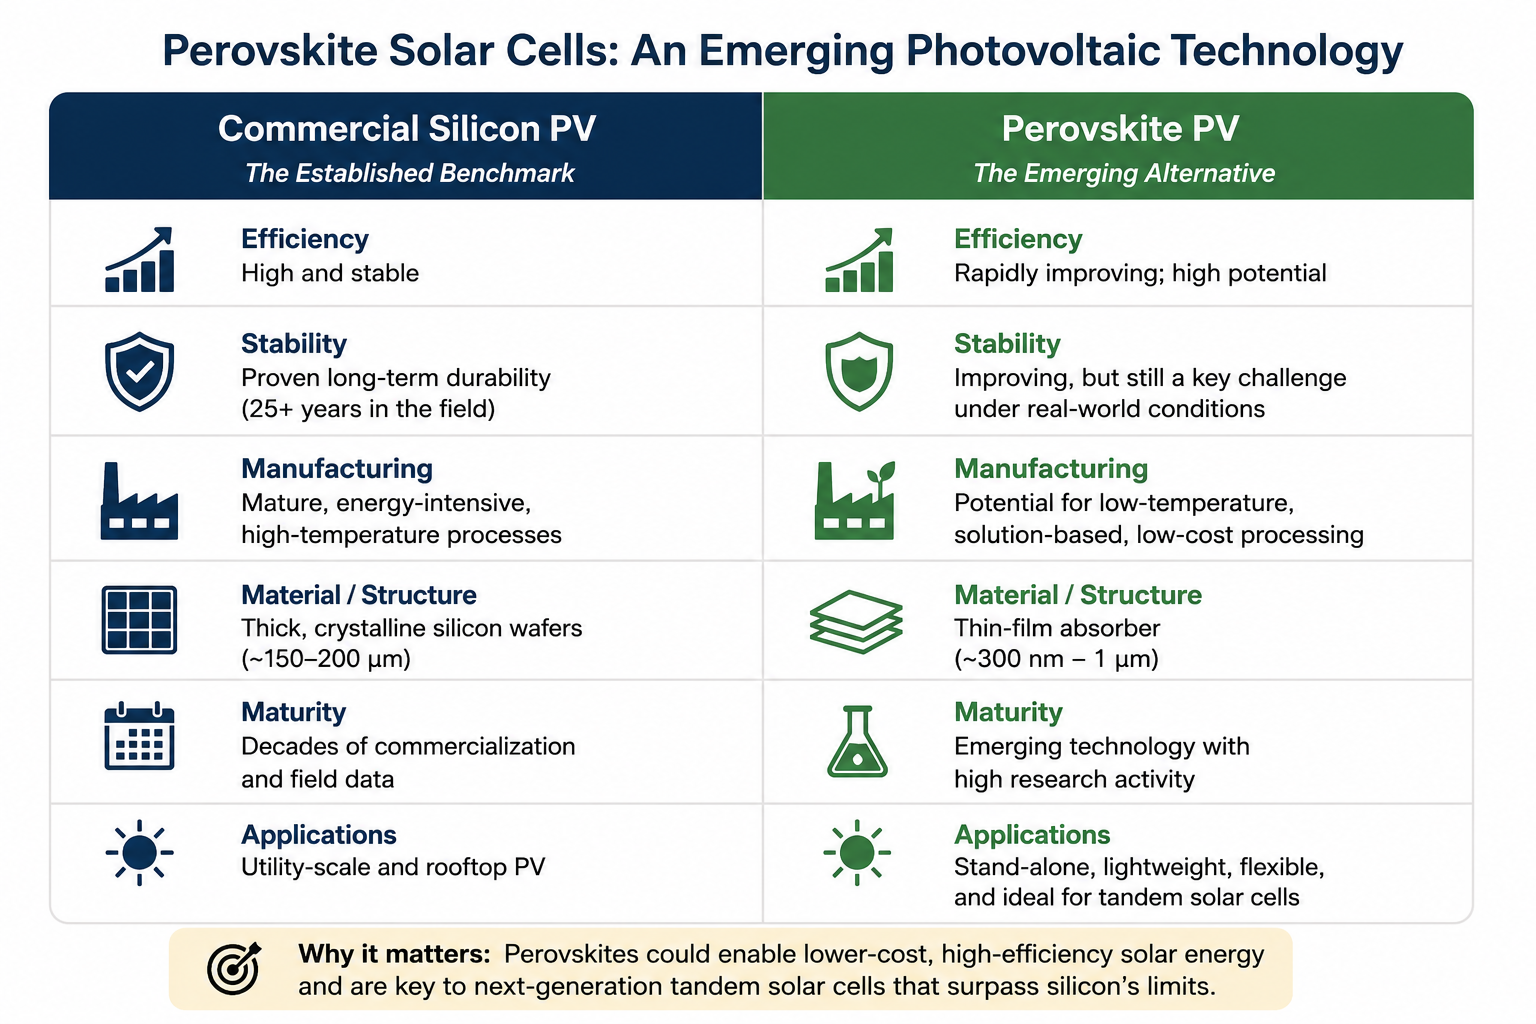
\includegraphics[width=0.92\textwidth]{figures/pptx_ai/si_vs_psc_comparison.png}
\caption{Qualitative comparison between mature commercial silicon photovoltaic
technology and emerging perovskite photovoltaics. The contrast motivates the
thesis focus: PSCs offer thin-film processing and tandem-cell potential, but
their operational stability remains the key barrier that must be understood
with device-physics and degradation modeling.}
\label{fig:si_vs_psc_comparison}
\end{figure}

This thesis develops a model in COMSOL Multiphysics, a finite-element
simulation environment, that connects measurable J--V behavior to hidden
internal mechanisms in a one-dimensional PSC stack. The model combines
electronic transport, internal electric fields, ion movement, degradation
variables, and resistance changes. Hysteresis is used in its standard PSC sense:
the measured J--V curve can depend on scan direction, scan rate, and voltage
history because internal ions and fields continue to evolve during the
measurement. The goal is not to fit one degradation curve with a trend line.
The goal is to build a model whose geometry, parameters, test conditions,
internal states, and outputs can be checked against physical expectations.

\section{Research Objective}

The objective is to develop a physics-based COMSOL model for PSC degradation
analysis. The model links observable J--V behavior to internal quantities such
as ion movement, defect growth, contact degradation, and leakage. It is
designed for future calibration against
experimental J--V, aging, impedance, transient-current, and optical data.
Impedance here means a small-signal electrical measurement that probes slow
charge, ion, and interface responses beyond a single J--V sweep. The claims in
this thesis are limited to the COMSOL model and the simulation results
reported in the following chapters.

\begin{figure}[H]
\centering
\includegraphics[width=\textwidth]{figures/pptx_ai/workflow_for_comsol_modeling_testing.png}
\caption{COMSOL modeling and testing workflow used in this thesis. A pristine
p-i-n model is compared with experimental J--V, EIS, transient-current, and
aging data; model parameters are calibrated; mobile-ion and degradation
physics are then used to predict J--V evolution and spatial state profiles.}
\label{fig:comsol_methodology_workflow}
\end{figure}

\section{Thesis Contributions}

The first contribution is a COMSOL device model based on a one-dimensional
version of the laboratory p-i-n stack. A p-i-n stack contains a p-selective
side, an intrinsic or weakly doped absorber, and an n-selective side. From the
illuminated substrate side, the physical device stack is
\begin{equation}
\mathrm{glass}/\mathrm{ITO}/\mathrm{NiO}_x/
\mathrm{MeO\mbox{-}2PACz}/\mathrm{MHP}/
\mathrm{C}_{60}/\mathrm{BCP}/\mathrm{Ag}/
\mathrm{UV\ resin}/\mathrm{glass}.
\end{equation}
Here ITO is indium tin oxide, NiO$_x$ is nickel oxide, MeO-2PACz is a
self-assembled monolayer used for hole extraction, MHP denotes the metal-halide
perovskite absorber, C$_{60}$ is fullerene, BCP is bathocuproine, and Ag is
silver.
The nominal values used in the laboratory description are approximately
30 nm NiO$_x$, 5 nm MeO-2PACz, 25 nm C$_{60}$, 4 nm BCP, 100 nm Ag, and
1.1 mm cover glass. In the COMSOL electrical model, the two hole-transport
layers are treated as one 35 nm hole-transport layer (HTL), C$_{60}$ and BCP
are treated as one 29 nm electron-transport layer (ETL), and the perovskite
absorber is 450 nm thick. ITO and Ag are the electrical contacts. Glass and UV
resin are part of the physical device, but they are not included as electronic
transport layers in the present model.
The Semiconductor Module solves the electronic device behavior, while
user-defined physics represent ion movement and gradual damage.

The second contribution is a set of degradation-mechanism parameter mappings.
The model maps hidden damage into quantities that COMSOL can use directly,
including defect density, ion charge density, series resistance, shunt
resistance, interface carrier loss, and light-generated current. Each mapping
has a physical meaning, a unit check, and an expected J--V signature.

The third contribution is a voltage-protocol method for aging and
hysteresis studies. The model separates the aging voltage
$V_{\mathrm{stress}}$ from the measurement scan voltage
$V_{\mathrm{app}}(t)$. This allows slow degradation and fast J--V scanning to
be modeled on different timescales. Multi-rate hysteretic J--V measurements are
used as calibration targets for the COMSOL degradation model.

The fourth contribution is an experimental comparison. The COMSOL
baseline and accelerated light-plus-heat degradation case are compared against
laboratory J--V data. The comparison evaluates direction, curve shape, PCE
loss, fill-factor loss, and calibration gaps rather than claiming absolute
lifetime prediction.

The fifth contribution is a first architecture-scoped stress grid for future
surrogate and inverse-model development. A surrogate model is a faster
data-driven approximation trained on COMSOL outputs, while an inverse model is
intended to infer internal device states from measured outputs. The canonical
6 $\times$ 6
light-temperature J--V sweep quantifies how accelerated aging metrics change
across coupled thermal and illumination stress. The matching profile grid
records ion, defect, recombination, electric-field, and resistance states
through the device. These outputs are not yet a final trained predictive
model, but they define the simulation data structure needed for one.

\section{Scope Boundaries}

The main thesis centers on the COMSOL model, the degradation mappings, and the
simulation results. A lightweight COMSOL-trained surrogate baseline is included
only to test whether the simulation data can train a forward model. It is not
presented as an experimentally calibrated lifetime predictor. The final claims
are therefore limited to mechanism separation within the simulated model and
to the data requirements for later calibration, inverse diagnosis, and
uncertainty analysis.

\section{Structure of the Thesis}

Chapter 2 summarizes the perovskite device physics and degradation mechanisms
needed to interpret the model. Chapter 3 defines the one-dimensional COMSOL
device geometry, material parameters, light-absorption model, ion equation, and
J--V metric extraction workflow. Chapter 4 describes the aging, hysteresis, and
transient-ion protocols used to separate slow degradation from fast electrical
measurement. Chapter 5 introduces the mappings that connect hidden defect,
contact, leakage, interface-loss, and light-generation changes to
observable J--V signatures.

Chapter 6 compares the model against experimental J--V and aging data to define
calibration targets and remaining gaps. Chapter 7 reports the simulated aging
results, electronic sensitivity sweeps, architecture-stress grid, spatial
profiles, and the lightweight COMSOL-trained surrogate baseline. Chapter 8
summarizes the limitations, reproducibility path, data availability, and future
work. The appendices collect parameter tables, mechanism mappings, and
reproducibility details so that implementation specifics do not interrupt the
main technical narrative.

\chapter{Physical Model Requirements}

\section{Why PSCs Need Mechanistic Models}

Stability assessment for PSCs is difficult because degradation depends on
device architecture, stress protocol, preconditioning, and measurement history.
The ISOS consensus work formalized how stability tests should be reported, but
standardized testing does not remove the need for mechanism-aware models
\cite{Khenkin_2020}. A useful model must connect an observed electrical change
to a plausible internal cause without hiding uncertainty.

Drift-diffusion modeling is the natural starting point because it represents
carrier generation, recombination, transport, and electrostatics in the device
stack. Recent PSC modeling reviews emphasize that these models remain valuable
when assumptions are explicit and when electronic and ionic degrees of freedom
are not confused \cite{Singh_2025}. COMSOL is used here as the finite-element
environment for that device model, not as a black box.

\section{p-i-n Device Operation and J--V Observables}

The laboratory device is an inverted p-i-n architecture. Light enters through
the glass/ITO side, followed by the p-selective NiO$_x$/MeO-2PACz contact,
the nominally intrinsic metal-halide perovskite absorber, the n-selective
C$_{60}$/BCP contact, and the Ag electrode. Photons absorbed in the
perovskite generate electron--hole pairs. Holes are extracted toward
NiO$_x$/MeO-2PACz and ITO, while electrons are extracted toward C$_{60}$/BCP
and Ag.

The measured J--V curve compresses several physical processes into four common
metrics. The short-circuit current density $J_{sc}$ is most sensitive to
absorption and carrier collection. The open-circuit voltage $V_{oc}$ is
strongly constrained by recombination and energetic alignment. Fill factor
responds to recombination, transport barriers, series resistance, and shunt
leakage. PCE combines all three:
\begin{equation}
\mathrm{PCE}=\frac{V_{oc}J_{sc}\mathrm{FF}}{P_{\mathrm{in}}}.
\end{equation}
Because different internal changes can produce similar metric changes, the
full curve shape, scan direction, scan rate, and measurement history are
required for mechanism-aware interpretation.

\section{Electronic Transport Equations}

The electronic device physics are governed by Poisson electrostatics, carrier
continuity, and electron and hole current-density relations. The electric
potential $\phi$ defines the electric field
\begin{equation}
\mathbf{E}=-\nabla \phi .
\end{equation}
The electron and hole current densities are written as
\begin{align}
\mathbf{J}_n &= q\mu_n n\mathbf{E} + qD_n\nabla n,\\
\mathbf{J}_p &= q\mu_p p\mathbf{E} - qD_p\nabla p,
\end{align}
where $q$ is the elementary charge, $n$ and $p$ are electron and hole
concentrations, $\mu_n$ and $\mu_p$ are mobilities, and $D_n$ and $D_p$ are
diffusion coefficients. The drift terms follow the force on mobile charges
under $\mathbf{E}$, while the diffusion terms follow concentration gradients.
The opposite signs in the diffusion terms reflect the charge sign convention
for electrons and holes.

Carrier conservation is represented by
\begin{align}
\frac{\partial n}{\partial t}
&= \frac{1}{q}\nabla\cdot \mathbf{J}_n + G - R,\\
\frac{\partial p}{\partial t}
&= -\frac{1}{q}\nabla\cdot \mathbf{J}_p + G - R,
\end{align}
where $G$ is photogeneration and $R$ is the total recombination rate. The
different signs in the divergence terms follow from the definitions of
electron and hole conventional current.

Electrostatics is coupled through Poisson's equation:
\begin{equation}
\nabla\cdot(\epsilon\nabla\phi)
= -q\left(p-n+N_D^+-N_A^-+\frac{\rho_{\mathrm{ion}}}{q}\right).
\label{eq:poisson}
\end{equation}
Here $\epsilon$ is the permittivity, $N_D^+$ and $N_A^-$ are ionized donor and
acceptor densities, and $\rho_{\mathrm{ion}}$ is the mobile-ion space-charge
density in C/m$^3$. The expression $\rho_{\mathrm{ion}}/q$ converts ionic
charge density into an equivalent signed number density before multiplication
by $q$.

\section{Generation and Recombination Terms}

Illumination enters the Semiconductor Module as a volumetric electron-hole pair
generation rate $G$ in the perovskite absorber. The optical field is not solved
with a Wave Optics interface. Instead, the model uses an algebraic
Beer--Lambert generation profile that supplies a spatially varying source term
to the semiconductor equations. The photon flux entering the absorber is
represented as
\begin{equation}
\Phi(x)=\Phi_0 e^{-\alpha x},
\end{equation}
where $\Phi_0$ is the incident photon flux at the illuminated side of the
absorber, $\alpha$ is an effective absorption coefficient, and $x$ is the local
depth coordinate in the perovskite. The corresponding generation profile is
proportional to the decaying photon flux and is normalized so that the
absorber-averaged generation remains controlled. This approach preserves a
depth-dependent generation shape without requiring a full optical transfer
matrix. It does not resolve wavelength-dependent absorption, parasitic
absorption in transport layers, interference effects, or optical reflection.

The total electronic recombination rate can be organized as
\begin{equation}
R = R_{\mathrm{rad}}+R_{\mathrm{SRH}}+R_{\mathrm{Auger}}.
\end{equation}
Direct or bimolecular radiative recombination is represented by
\begin{equation}
R_{\mathrm{rad}}=B\left(np-n_i^2\right),
\end{equation}
where $B$ is the radiative recombination coefficient. Auger recombination can
be written as
\begin{equation}
R_{\mathrm{Auger}}=
\left(C_n n+C_p p\right)\left(np-n_i^2\right),
\end{equation}
where $C_n$ and $C_p$ are electron- and hole-assisted Auger coefficients.
Radiative and Auger terms define the complete recombination hierarchy presented
for the device physics, but the current degradation implementation is
calibrated primarily through SRH recombination. Future quantitative use of
$B$, $C_n$, and $C_p$ requires architecture-specific transient or
photoluminescence calibration.

Trap-assisted recombination is represented with the Shockley--Read--Hall (SRH)
form
\begin{equation}
R_{\mathrm{SRH}} =
\frac{np-n_i^2}
{\tau_p(n+n_1)+\tau_n(p+p_1)}.
\label{eq:srh}
\end{equation}
The carrier lifetimes depend on trap density:
\begin{align}
\tau_n &= \frac{1}{\sigma_n v_{\mathrm{th}} N_t},\\
\tau_p &= \frac{1}{\sigma_p v_{\mathrm{th}} N_t},
\end{align}
where $\sigma_n$ and $\sigma_p$ are capture cross sections, $v_{\mathrm{th}}$
is thermal velocity, and $N_t$ is trap density. Increasing $N_t$ reduces
carrier lifetime, increases nonradiative recombination, lowers $V_{oc}$, and
can reduce fill factor or $J_{sc}$ when recombination becomes strong.

\section{Hysteresis as a Modeling Requirement}

J--V hysteresis is an observable result of coupling among mobile ions, internal
electric fields, recombination, and voltage protocol. Huang et al. showed that
dielectric properties and scan rate can strongly affect PSC hysteresis, and
their time-dependent ion-migration model links those effects to built-in field
changes \cite{Huang_2022}. Wang et al. further argued that hysteresis can be
used diagnostically because evolving ion-induced fields interact with carrier
transport and recombination \cite{WangNatComm_2024}.

A model that only produces one steady J--V curve at one scan rate cannot test
whether the internal state is physically credible. Slower scans allow ionic
states to respond more fully; faster scans probe a more frozen internal state.
Agreement across scan protocols is therefore a stronger model-quality test than
agreement at one operating point.

\section{Model Requirements}

The COMSOL model uses the following requirements:
\begin{enumerate}
\item The device stack and contacts must be explicit enough for comparison to
laboratory samples.
\item Voltage protocol variables must be treated as controlled inputs, not as
hidden physics.
\item Internal material and degradation states must be represented as model
parameters or state variables, not inferred from PCE alone.
\item Mobile-ion redistribution must enter Poisson electrostatics through a
charge-density term with consistent units.
\item Degradation variables must map to COMSOL-accessible quantities such as
$N_t$, $R_s$, $R_{sh}$, surface recombination, and photogeneration.
\item Model claims must be limited to the parameter range, stress protocol, and
calibration state actually simulated.
\end{enumerate}

\chapter{COMSOL Model Development Workflow}

\section{COMSOL Multiphysics Framework}

COMSOL Multiphysics is a finite-element platform for solving coupled partial
differential equations on a shared geometry. In this work, the Semiconductor
interface solves electronic drift-diffusion and Poisson electrostatics, a
user-defined PDE solves mobile-ion transport, additional PDE or global states
represent degradation, and the Electrical Circuit interface represents lumped
series and shunt pathways. This organization keeps the conservation laws,
domain selections, boundary conditions, and coupling variables inspectable.

\section{Device Stack and Geometry}

The COMSOL model is organized around a one-dimensional PSC stack through the
layer-thickness direction. The physical laboratory architecture, listed from
the illuminated side, is
\begin{equation}
\mathrm{glass}/\mathrm{ITO}/\mathrm{NiO}_x/
\mathrm{MeO\mbox{-}2PACz}/\mathrm{MHP}/
\mathrm{C}_{60}/\mathrm{BCP}/\mathrm{Ag}/
\mathrm{UV\ resin}/\mathrm{glass}.
\end{equation}
The reduced active-device model is
\begin{equation}
\mathrm{ITO}/(\mathrm{NiO}_x+\mathrm{MeO\mbox{-}2PACz})/
\mathrm{Cs}_{0.2}\mathrm{FA}_{0.8}\mathrm{PbI}_3/
(\mathrm{C}_{60}+\mathrm{BCP})/\mathrm{Ag}.
\end{equation}

\begin{table}[H]
\centering
\caption{Laboratory architecture and reduced COMSOL representation.}
\label{tab:lab_comsol_stack}
\begin{tabular}{
>{\raggedright\arraybackslash}p{0.29\textwidth}
>{\raggedright\arraybackslash}p{0.23\textwidth}
>{\raggedright\arraybackslash}p{0.36\textwidth}}
\toprule
Laboratory layer & Nominal thickness & COMSOL treatment \\
\midrule
Front glass & substrate & omitted from electronic domain; defines illumination side \\
ITO & transparent electrode & electrical boundary contact at $x=0$ \\
NiO$_x$ & approximately 30 nm & combined into 35 nm p-type HTL \\
MeO-2PACz & approximately 5 nm & combined into 35 nm p-type HTL \\
Metal-halide perovskite & 450 nm model value & intrinsic absorber with Cs$_{0.2}$FA$_{0.8}$PbI$_3$ electronic parameters \\
C$_{60}$ & approximately 25 nm & combined into 29 nm n-type ETL \\
BCP & approximately 4 nm & combined into 29 nm n-type ETL \\
Ag & approximately 100 nm & electrical boundary contact \\
UV resin and cover glass & resin and 1.1 mm glass & omitted from electronic domain \\
\bottomrule
\end{tabular}
\end{table}

Transport layers, absorber, interfaces, and contacts are retained as explicit
electronic model objects at the resolution needed for carrier transport.
Contacts are applied as electrical boundaries. The
one-dimensional assumption removes lateral nonuniformity and treats the device
as laterally homogeneous, which is appropriate for mechanism development but
cannot resolve pinholes, local shunts, edge effects, or grain-scale
heterogeneity.

Some historical COMSOL objects and the May 31, 2026 MATLAB export retain
legacy labels such as ``FTO/Contact'' and ``Au/Contact.'' Those labels do not
define the physical device used in this thesis. They must be interpreted and
renamed as the illuminated ITO contact and rear Ag contact before final
device-specific calibration.

\begin{figure}[H]
\centering
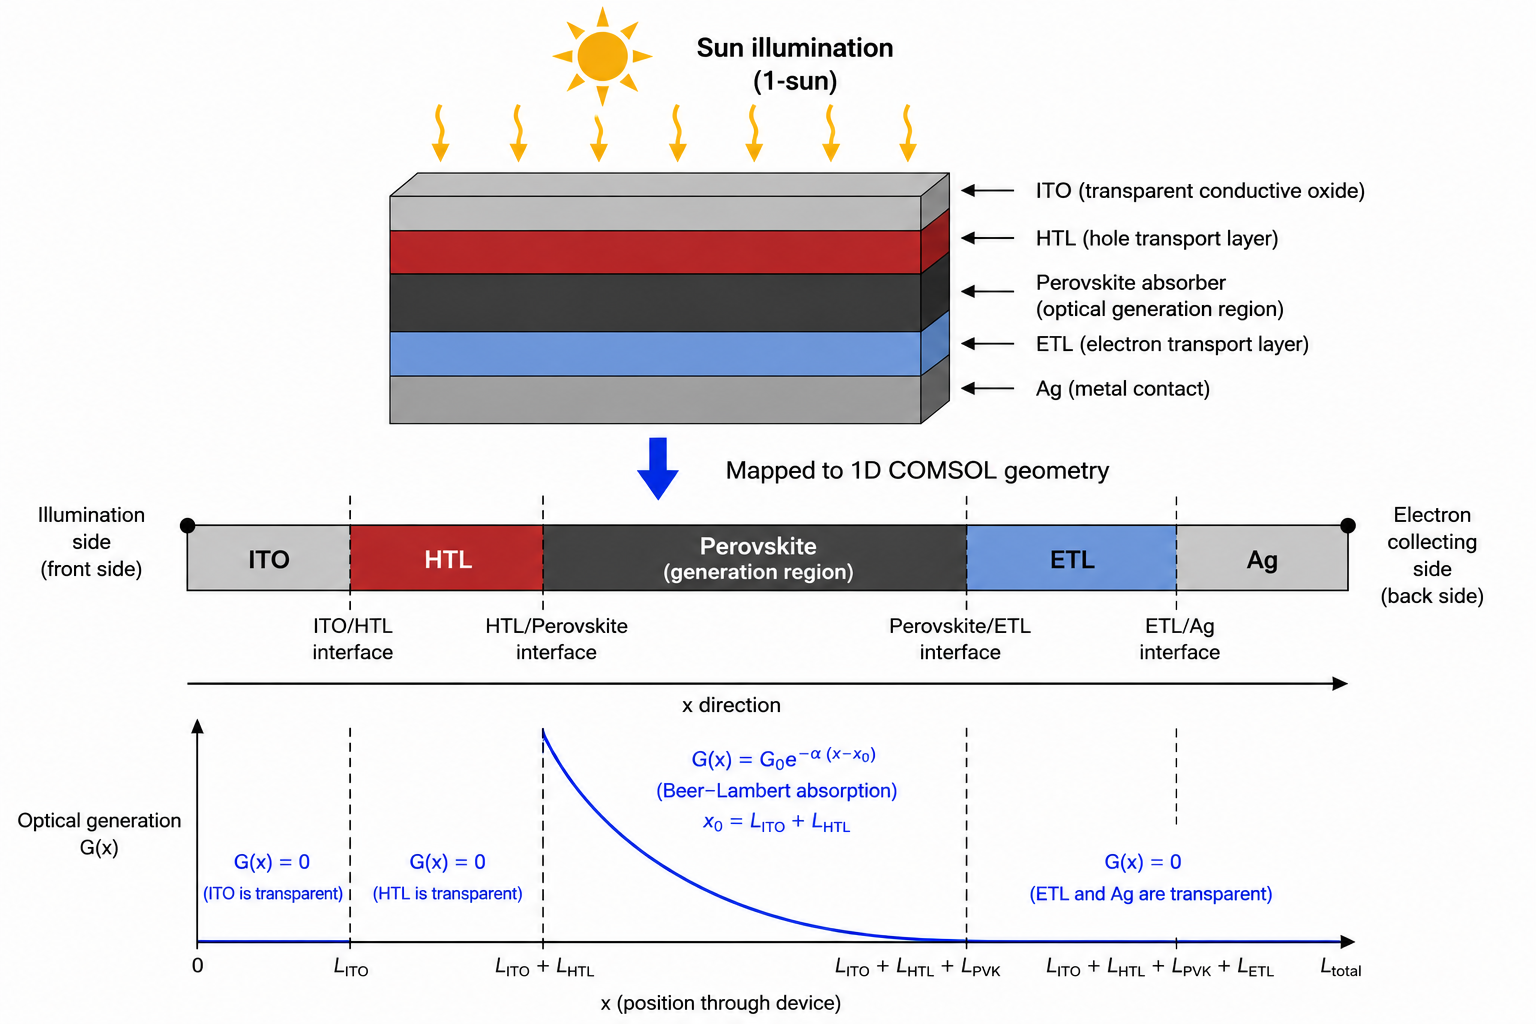
\includegraphics[width=0.96\textwidth]{figures/pptx_ai/psc_architecture_illumination_1d_mapping.png}
\caption{Laboratory p-i-n device architecture and its reduced 1-D COMSOL
mapping. Illumination enters from the ITO/HTL side, the transport layers and
absorber are mapped onto the model $x$ direction, and optical generation is
applied only in the perovskite absorber using the Beer--Lambert profile
implemented below.}
\label{fig:psc_stack_geometry}
\end{figure}

\section{Semiconductor Module Implementation}

The Semiconductor Module solves the coupled electronic transport problem by
assembling Poisson's equation, electron and hole continuity equations, and
current-density relations on the one-dimensional mesh \cite{comsol64}. Material
properties such as relative permittivity, mobility, band gap, electron affinity,
effective density of states, recombination lifetime, and trap density are
assigned by domain. For the laboratory architecture used here, the electrical
boundaries represent ITO at the illuminated side and Ag at the rear side. The target
coordinate convention is $x=0$ at ITO/HTL and increasing through the
perovskite toward ETL/Ag.

The primary dependent variables are the electrostatic potential and carrier
concentrations or quasi-Fermi-level variables, depending on the COMSOL
formulation selected in the model. The physical role is the same in either
formulation: COMSOL solves the nonlinear drift-diffusion system so that the
terminal current density is consistent with electrostatics, generation,
recombination, and boundary injection. The solver output is a simulated J--V
curve for the selected voltage protocol and internal state.

\begin{figure}[H]
\centering
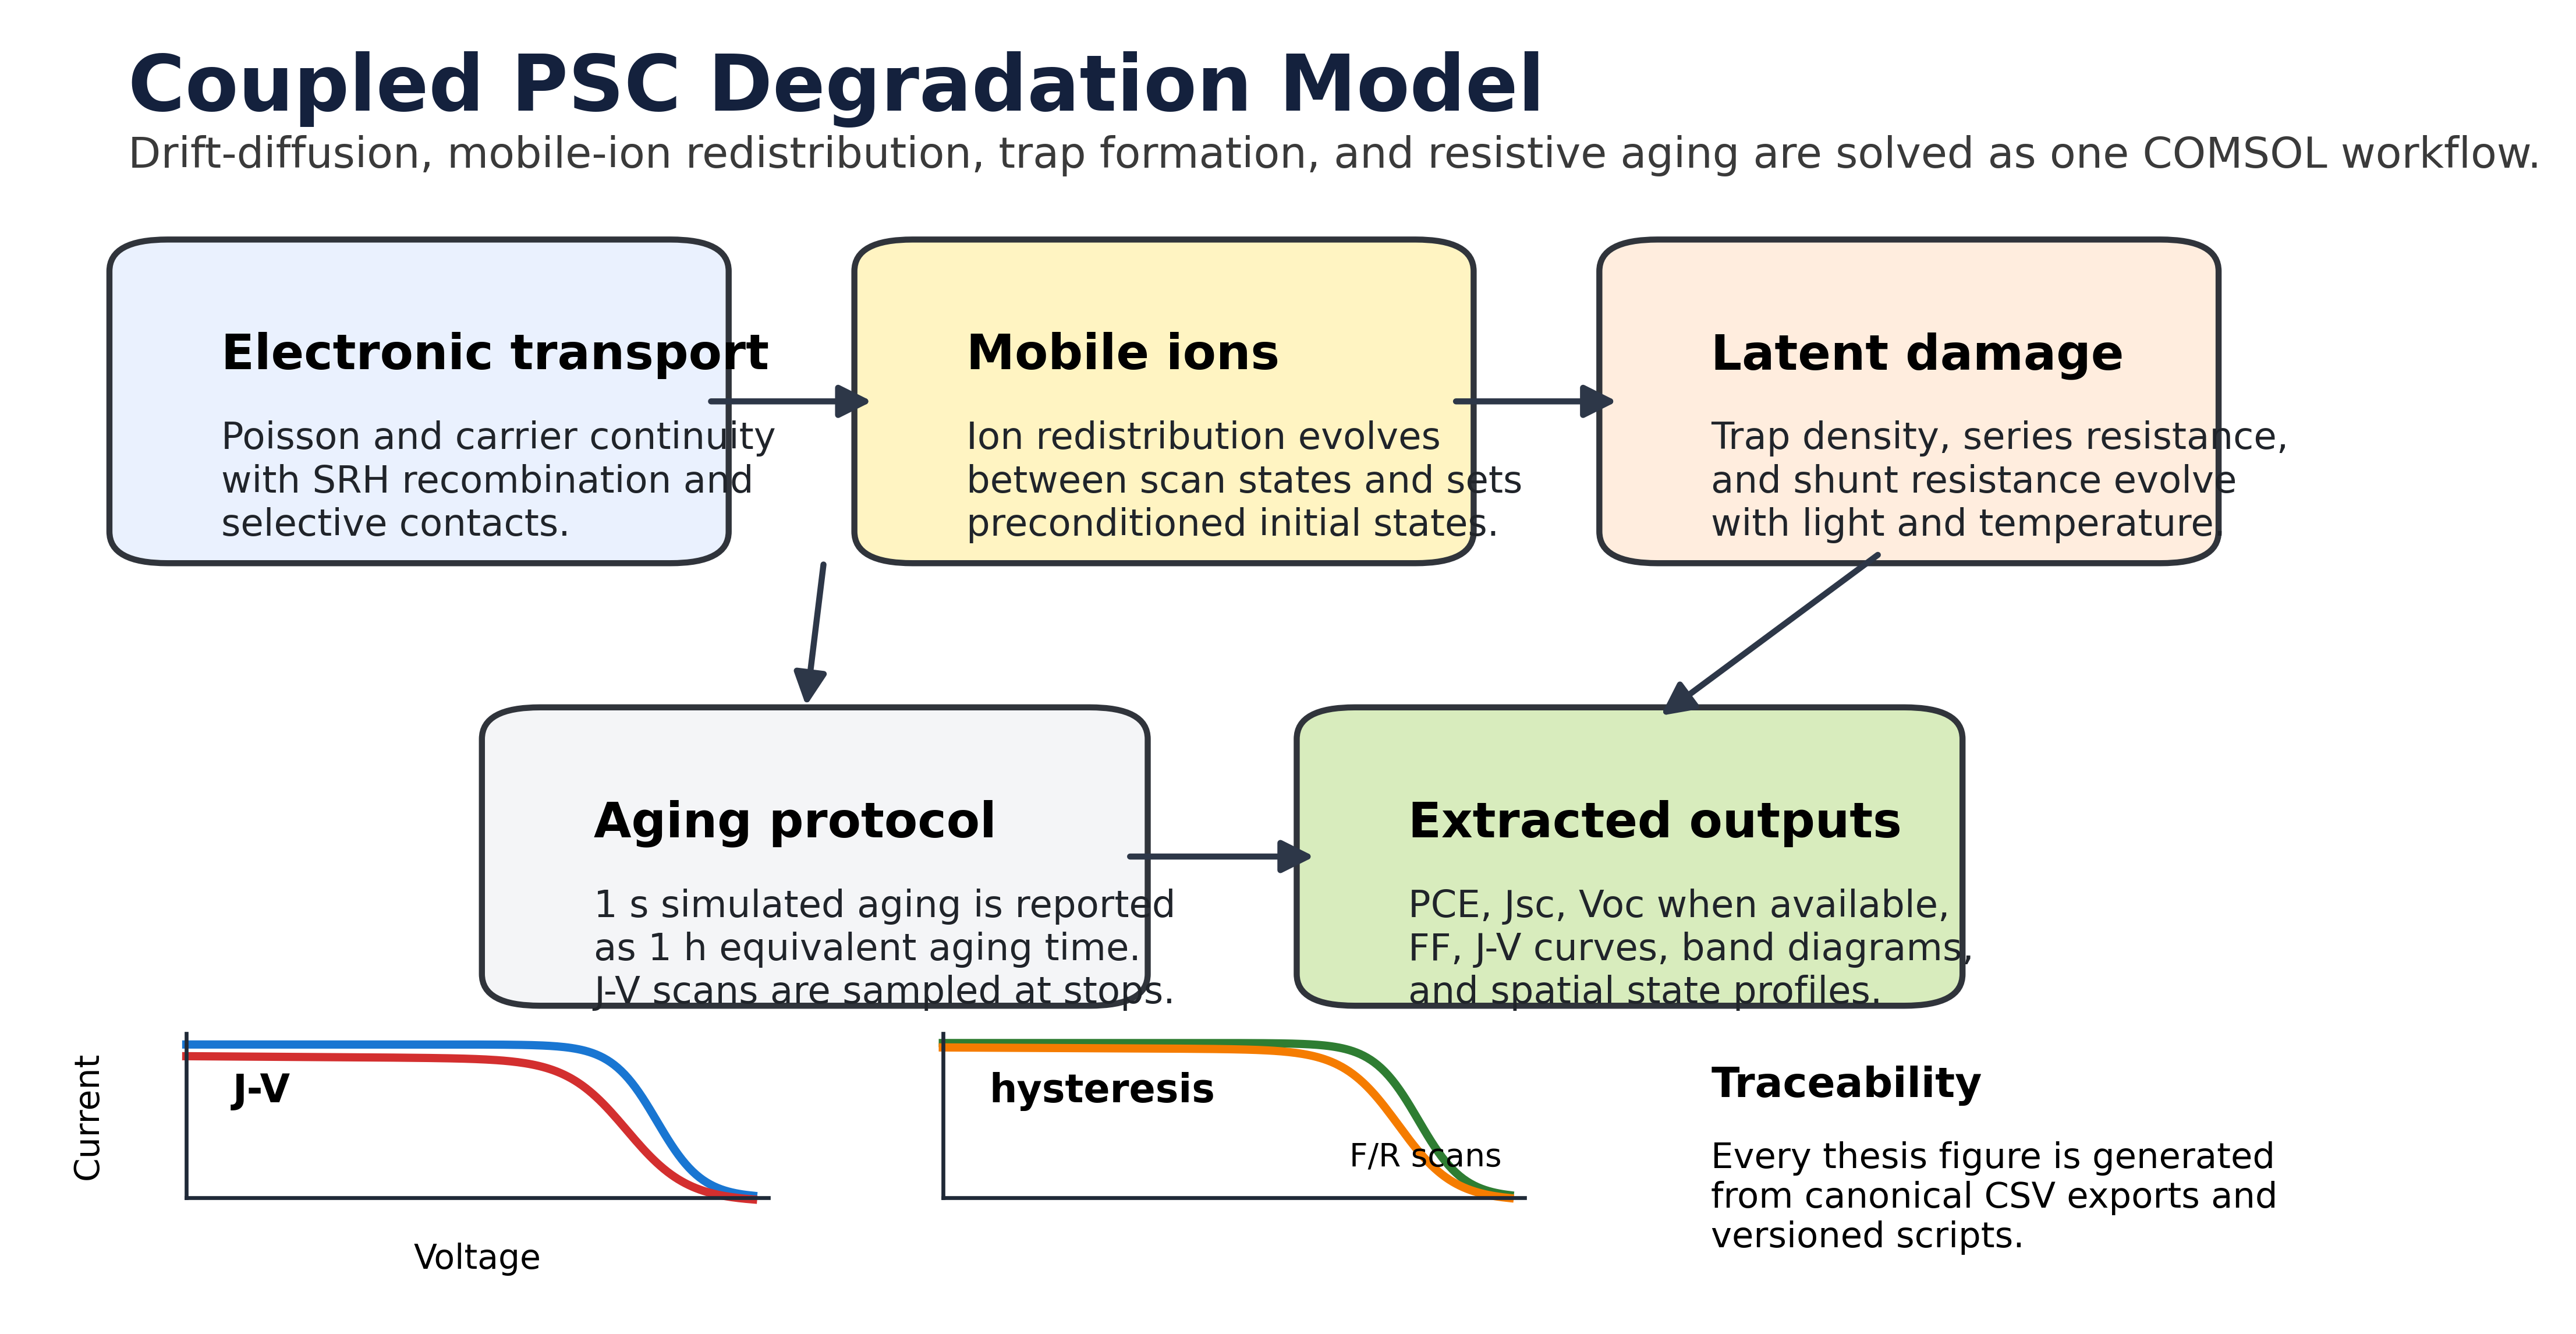
\includegraphics[width=\textwidth]{figures/pptx_ai/coupled_physics_workflow.png}
\caption{Coupled-physics structure of the COMSOL model. Electrostatics drives electronic transport and mobile-ion migration; ion redistribution feeds back through the electrostatic source term; degradation states modify recombination and transport parameters; the outputs include J--V curves, hysteresis, internal fields, and aging trends.}
\label{fig:coupled_physics_workflow}
\end{figure}

\section{Optical Generation Model}

The Semiconductor Module requires a volumetric electron-hole pair generation
rate in the perovskite absorber. The COMSOL implementation does not solve the
optical field with the Wave Optics interface. Optical absorption is represented
with an algebraic Beer--Lambert profile that is supplied directly to the
Semiconductor interface as a source term. The formulation is used in the
one-dimensional p-i-n stack
\begin{equation}
\mathrm{ITO}/(\mathrm{NiO}_x+\mathrm{MeO\mbox{-}2PACz})/
\mathrm{Cs}_{0.2}\mathrm{FA}_{0.8}\mathrm{PbI}_3/
(\mathrm{C}_{60}+\mathrm{BCP})/\mathrm{Ag},
\end{equation}
with active-layer dimensions
\begin{align}
\mathrm{thickness}_{\mathrm{ETL}} &= 29~\mathrm{nm},\\
\mathrm{thickness}_{\mathrm{PVK}} &= 450~\mathrm{nm},\\
\mathrm{thickness}_{\mathrm{HTL}} &= 35~\mathrm{nm},\\
A &= 9\times10^{-6}~\mathrm{m^2}.
\end{align}

The Beer--Lambert approximation assumes that the photon flux decays
exponentially through the absorber:
\begin{equation}
I(x)=I_0 e^{-\alpha_{\mathrm{pvk}}x_{\mathrm{pvk}}},
\end{equation}
where $I_0$ is the optical intensity entering the perovskite,
$\alpha_{\mathrm{pvk}}$ is the effective absorber absorption coefficient, and
$x_{\mathrm{pvk}}$ is the local depth measured from the illuminated
perovskite interface. The absorbed optical power density is
\begin{equation}
P_{\mathrm{abs}}(x_{\mathrm{pvk}})
=\alpha_{\mathrm{pvk}} I_0 e^{-\alpha_{\mathrm{pvk}}x_{\mathrm{pvk}}}.
\end{equation}
Using an effective photon energy
\begin{equation}
E_{\mathrm{ph}}=\frac{hc}{\lambda_{\mathrm{eff}}},
\end{equation}
the volumetric electron-hole pair generation rate becomes
\begin{equation}
G_{\mathrm{opt}}(x_{\mathrm{pvk}})
=\frac{\alpha_{\mathrm{pvk}}I_0\lambda_{\mathrm{eff}}}{hc}
e^{-\alpha_{\mathrm{pvk}}x_{\mathrm{pvk}}}.
\label{eq:beer_lambert_physical}
\end{equation}
This expression has units of m$^{-3}$s$^{-1}$ when $I_0$ is in W/m$^2$,
$\alpha_{\mathrm{pvk}}$ is in m$^{-1}$, and $\lambda_{\mathrm{eff}}$ is in m.
The direct COMSOL variable set for this physical form is
\texttt{alpha\_pvk}, \texttt{I0}, \texttt{lambda\_eff},
\texttt{Ephoton}, \texttt{x\_pvk}, and \texttt{Gopt}. The current model uses the
same Beer--Lambert depth dependence as a normalized algebraic shape so that
photogeneration can be calibrated independently from the front/back absorption
contrast.

The local perovskite coordinate is
\begin{equation}
x_{\mathrm{pvk}}=x-x_{\mathrm{pvk},0},
\end{equation}
with
\begin{equation}
x_{\mathrm{pvk},0}=\mathrm{thickness\_ETL},
\qquad
L_{\mathrm{gen}}=\mathrm{thickness\_PVK}.
\end{equation}
To avoid evaluating the exponential outside the perovskite domain, the local
coordinate is clipped:
\begin{equation}
x_{\mathrm{clip}}=
\min\left(\max\left(x_{\mathrm{pvk}},0\right),L_{\mathrm{gen}}\right).
\end{equation}

The raw dimensionless Beer--Lambert shape is
\begin{equation}
S_{\mathrm{raw}}(x)=e^{-\alpha_{\mathrm{gen}}x_{\mathrm{clip}}}.
\end{equation}
For numerical stability, COMSOL applies a small floor:
\begin{equation}
S_{\mathrm{raw}}(x)=
\max\left(e^{-\alpha_{\mathrm{gen}}x_{\mathrm{clip}}},
S_{\mathrm{floor}}\right).
\end{equation}
The analytical average of the unbounded exponential shape over the absorber is
\begin{equation}
\left\langle S_{\mathrm{raw}}\right\rangle =
\frac{1}{L_{\mathrm{gen}}}
\int_0^{L_{\mathrm{gen}}}e^{-\alpha_{\mathrm{gen}}x}\,dx,
\end{equation}
which gives
\begin{equation}
\left\langle S_{\mathrm{raw}}\right\rangle =
\frac{1-e^{-\alpha_{\mathrm{gen}}L_{\mathrm{gen}}}}
{\alpha_{\mathrm{gen}}L_{\mathrm{gen}}}.
\end{equation}
The normalized generation shape is
\begin{equation}
S_{\mathrm{norm}}(x)=
\frac{S_{\mathrm{raw}}(x)}
{\max\left(\left\langle S_{\mathrm{raw}}\right\rangle,
S_{\mathrm{floor}}\right)}.
\end{equation}
This normalization makes the spatial average of the shape approximately unity,
so the generation profile changes the depth distribution of photogeneration
without unintentionally changing the integrated generation strength.

The final optical generation rate is
\begin{equation}
G_{\mathrm{opt}}(x)=
G_0 S_{\mathrm{scale}}S_{\mathrm{norm}}(x).
\end{equation}
In the COMSOL variable set, this is implemented as
\begin{center}
\texttt{Gopt = G0\_0*Gshape\_scale*Gshape\_norm}.
\end{center}
The variables \texttt{Gshape\_raw}, \texttt{Gshape\_avg}, and \texttt{Gshape\_norm} are
dimensionless. \texttt{Gopt} has the same units as \texttt{G0\_0}, typically
1/(m$^3$s). If separate electron and hole generation fields are required by the
Semiconductor interface, both use the same algebraic expression,
\texttt{Gopt}. \texttt{Gopt} is not a solved dependent variable.

\begin{table}[H]
\centering
\footnotesize
\caption{COMSOL parameters for the algebraic Beer--Lambert generation profile.}
\label{tab:beer_lambert_parameters}
\begin{tabular}{p{0.20\textwidth}p{0.34\textwidth}p{0.36\textwidth}}
\toprule
Parameter & Expression & Meaning \\
\midrule
\texttt{alpha\_gen} & \texttt{5e6[1/m]} & Effective Beer--Lambert absorption coefficient \\
\texttt{Gshape\_floor} & \texttt{1e-6} & Numerical floor for the generation shape \\
\texttt{Gshape\_scale} & \texttt{1} & Manual generation calibration multiplier \\
\texttt{x\_pvk0} & \texttt{thickness\_ETL} & Start coordinate of the perovskite layer \\
\texttt{x\_pvk1} & \texttt{thickness\_ETL + thickness\_PVK} & End coordinate of the perovskite layer \\
\texttt{Lgen} & \texttt{thickness\_PVK} & Optical generation thickness \\
\bottomrule
\end{tabular}
\end{table}

\begin{table}[H]
\centering
\footnotesize
\caption{COMSOL variables for the normalized Beer--Lambert generation source.}
\label{tab:beer_lambert_variables}
\begin{tabular}{p{0.18\textwidth}p{0.48\textwidth}p{0.24\textwidth}}
\toprule
Variable & COMSOL expression & Meaning \\
\midrule
\texttt{xpvk} & \texttt{x-x\_pvk0} & Local coordinate into the perovskite \\
\texttt{xpvk\_clip} & \texttt{min(max(xpvk,0[m]),Lgen)} & Clipped local coordinate \\
\texttt{Gshape\_raw} &
\begin{tabular}[t]{@{}l@{}}
\texttt{max(exp(-alpha\_gen*xpvk\_clip),}\\
\texttt{Gshape\_floor)}
\end{tabular}
& Raw Beer--Lambert shape \\
\texttt{Gshape\_avg} &
\begin{tabular}[t]{@{}l@{}}
\texttt{(1-exp(-alpha\_gen*Lgen))/}\\
\texttt{(alpha\_gen*Lgen)}
\end{tabular}
& Analytical average of the exponential profile \\
\texttt{Gshape\_norm} &
\begin{tabular}[t]{@{}l@{}}
\texttt{Gshape\_raw/max(Gshape\_avg,}\\
\texttt{Gshape\_floor)}
\end{tabular}
& Normalized generation shape \\
\texttt{Gopt} & \texttt{G0\_0*Gshape\_scale*Gshape\_norm} & Final optical generation rate \\
\bottomrule
\end{tabular}
\end{table}

For \texttt{alpha\_gen = 5e6[1/m]} and
\texttt{Lgen = 450[nm]},
\begin{equation}
\alpha_{\mathrm{gen}}L_{\mathrm{gen}}
=5\times10^6 \times 450\times10^{-9}=2.25.
\end{equation}
The raw back/front generation ratio is therefore
\begin{equation}
e^{-2.25}\approx0.105.
\end{equation}
Before normalization, generation at the back of the absorber is about 10.5\%
of the generation near the illuminated side. For
\texttt{alpha\_gen = 1e7[1/m]},
\begin{equation}
\alpha_{\mathrm{gen}}L_{\mathrm{gen}}=4.5,
\end{equation}
and
\begin{equation}
e^{-4.5}\approx0.011.
\end{equation}
The profile is then much more front-loaded. The parameter
\texttt{alpha\_gen} is therefore treated as an effective
calibration/sensitivity parameter rather than a fully resolved optical
constant.

The generation profile should first be plotted over the perovskite domain to
confirm that it decreases monotonically from the illuminated side and remains
finite. The J--V curve should then be compared against the calibrated baseline
to evaluate changes in \texttt{Jsc}, \texttt{Voc}, \texttt{FF}, \texttt{PCE},
carrier-density profiles, recombination profiles, and local degradation
drivers.

\section{Mobile-Ion PDE}

Mobile ions are represented with a user-defined drift-diffusion equation,
consistent with mixed ionic-electronic PSC modeling practice
\cite{Richardson_2016,Calado_2022_Driftfusion}. For an ionic concentration
$c_{\mathrm{ion}}$, conservation gives
\begin{equation}
\frac{\partial c_{\mathrm{ion}}}{\partial t}
= -\nabla\cdot\mathbf{N}_{\mathrm{ion}},
\end{equation}
with Nernst--Planck flux
\begin{equation}
\mathbf{N}_{\mathrm{ion}}
= -D_{\mathrm{ion}}\nabla c_{\mathrm{ion}}
- \mu_{\mathrm{ion}} z_{\mathrm{ion}} q c_{\mathrm{ion}}\nabla\phi .
\label{eq:ion_flux}
\end{equation}
Here $D_{\mathrm{ion}}$ is ion diffusivity in m$^2$/s, $\mu_{\mathrm{ion}}$ is
ion mobility in m$^2$/(V s), $z_{\mathrm{ion}}$ is the signed ion valence, and
$\mathbf{N}_{\mathrm{ion}}$ has units of m$^{-2}$s$^{-1}$. Since
$\mathbf{E}=-\nabla\phi$, the migration term may also be written as
$\mu_{\mathrm{ion}} z_{\mathrm{ion}} q c_{\mathrm{ion}}\mathbf{E}$ depending
on sign convention. The implemented convention must match the sign of
$z_{\mathrm{ion}}$ and the direction of the electric field in COMSOL.

The dependent variable used in the General Form PDE interface is the normalized
ion state
\begin{equation}
u_{\mathrm{ion}}=\frac{c_{\mathrm{ion}}}{c_{\mathrm{ion},0}},
\qquad
c_{\mathrm{ion}}=c_{\mathrm{ion},0}u_{\mathrm{ion}},
\end{equation}
where $c_{\mathrm{ion},0}$ is the initial mobile-ion concentration. Substituting
into the conservation equation gives
\begin{equation}
\frac{\partial u_{\mathrm{ion}}}{\partial t}
=
\nabla\cdot\left[
D_{\mathrm{ion}}\nabla u_{\mathrm{ion}}
+ \mu_{\mathrm{ion}} z_{\mathrm{ion}} q u_{\mathrm{ion}}\nabla\phi
\right].
\label{eq:normalized_ion}
\end{equation}
The normalized state is dimensionless, so each term in
Eq.~\ref{eq:normalized_ion} has units of 1/s. In COMSOL, this equation is
implemented in the perovskite domain using the electrostatic potential from the
Semiconductor Module as a coupled field.

For one-dimensional implementation and diagnostics, it is useful to write the
normalized ion flux in terms of the electric field used to drive migration:
\begin{equation}
\Gamma_u
=-\frac{\partial u_{\mathrm{ion}}}{\partial x}
+\frac{z_{\mathrm{ion}}q}{k_{\mathrm{B}}T}
u_{\mathrm{ion}}E_{\mathrm{ion}} .
\label{eq:normalized_ion_flux}
\end{equation}
Here $E_{\mathrm{ion}}$ is the actual field supplied to the ion equation in
V/m. The corresponding physical particle flux and ionic current density are
\begin{align}
N_{\mathrm{ion}} &=D_{\mathrm{ion}}c_{\mathrm{ion},0}\Gamma_u,\\
J_{\mathrm{ion}} &=z_{\mathrm{ion}}qN_{\mathrm{ion}} .
\end{align}
These forms provide direct unit checks: $N_{\mathrm{ion}}$ has units
m$^{-2}$s$^{-1}$ and $J_{\mathrm{ion}}$ has units A/m$^2$.

The ionic charge density coupled into Poisson electrostatics is
\begin{equation}
\rho_{\mathrm{ion}}
=
\gamma_{\mathrm{ion}} q z_{\mathrm{ion}} c_{\mathrm{ion},0}
\left(u_{\mathrm{ion}}-1\right).
\label{eq:rho_ion}
\end{equation}
The factor $\gamma_{\mathrm{ion}}$ is a scaling or participation factor used to
control how strongly the normalized ion redistribution perturbs electrostatics.
The term $(u_{\mathrm{ion}}-1)$ is used so that a spatially uniform initial ion
distribution does not create artificial net space charge. Only redistribution
away from the initial uniform state contributes to the electrostatic source
term. The default ion boundary condition is blocking flux at the perovskite
interfaces unless an interfacial exchange model is explicitly specified.

\section{Mobile-Ion Preconditioning}

Perovskite devices do not enter a J--V scan from a unique uniform ionic state.
Bias history, illumination, and rest conditions redistribute mobile defects
before the measurement begins, and that ionic profile can screen or reinforce
the internal field during the subsequent voltage protocol
\cite{Eames_2015,Richardson_2016,Calado_2016}. The COMSOL workflow therefore
treats ion preconditioning as part of the initial condition rather than as a
post-processing correction.

The preconditioning sequence is:
\begin{enumerate}
\item solve the electronic stack at the selected dark or illuminated operating
condition;
\item run a time-dependent ion-relaxation study at the chosen history voltage
or open-circuit condition;
\item use the final $u_{\mathrm{ion}}(x,t_{\mathrm{pre}})$ distribution as the
initial condition for the J--V, hysteresis, or DIT study; and
\item verify ion conservation by checking that the absorber average of
$u_{\mathrm{ion}}$ remains close to unity.
\end{enumerate}
The same check should also inspect the maximum and minimum values of
$u_{\mathrm{ion}}$, the interfacial flux, and the resulting
$\rho_{\mathrm{ion}}$ profile. Large boundary spikes often indicate that the
field scaling, mesh, time stepping, or blocking boundary condition is forcing
an unphysical double layer.

In the COMSOL implementation, the electric-field expression supplied to the
ion equation must be consistent with the plotted electrostatic potential. The
symbolic derivative \texttt{d(V,x)} can evaluate to zero or to an unintended
field if the selected dependent variable is not the Semiconductor Module
potential. The Semiconductor Module field component, \texttt{semi.Ex}, is the
preferred diagnostic because it is consistent with the potential slope plotted
from the solved semiconductor physics. When additional numerical stabilization
or applied-bias control is needed, the ion-driving field is written as
\begin{equation}
E_{\mathrm{ion}}
=\eta_{E,\mathrm{bi}}E_{\mathrm{semi},x}
+\eta_{\mathrm{app}}\frac{V_{\mathrm{drive}}}{L_{\mathrm{pvk}}},
\end{equation}
where $E_{\mathrm{semi},x}$ is taken from \texttt{semi.Ex},
$L_{\mathrm{pvk}}$ is the perovskite thickness, and the dimensionless
$\eta$ factors are calibration and stabilization factors. For a 500 nm
absorber, a field of $10^6$ V/m corresponds to a 0.5 V potential drop, while
$k_{\mathrm{B}}T/q$ is only about 25.9 mV at room temperature. Unscaled fields
can therefore imply very large Boltzmann concentration ratios. Practical
preconditioning studies require bounded ion variables, conservative flux
settings, mesh refinement near interfaces, and comparison against
ion-sensitive measurements before the extracted ion concentration is treated
as unique.

\section{Stress-Dependent Mobile-Ion Transport and Degradation Coupling}

The mobile-ion model is extended from a static degradation-parameter
description into a dynamic stress-dependent formulation. Mobile-ion
redistribution is treated as a reversible, or partially reversible,
fast-to-medium-time-scale process. Material degradation is treated as a slower
irreversible process driven by stressors such as heat, illumination, electric
field, and local ion accumulation. This separation is important for calibration:
the model should first reproduce mobile-ion transport, then add one
degradation channel at a time. The first irreversible channel used for model
development is trap-density growth because it couples directly to SRH
recombination and therefore affects $V_{oc}$, FF, and PCE.

\subsection{Temperature and Light Dependence}

Mobile-ion diffusivity is thermally activated in hybrid lead iodide
perovskites, with iodide-related vacancy migration often treated as a dominant
fast ionic pathway \cite{Eames_2015,Futscher_2019}. The diffusivity is written
relative to a reference value:
\begin{equation}
D_{\mathrm{ion}}(T)
=D_{\mathrm{ion,ref}}
\exp\left[
-\frac{E_{a,\mathrm{ion}}}{k_{\mathrm{B}}}
\left(\frac{1}{T}-\frac{1}{T_{\mathrm{ref}}}\right)
\right].
\end{equation}
When the activation energy is entered in electron-volts, the COMSOL expression
uses $k_{\mathrm{B,eV}}=8.617333262\times10^{-5}$ eV/K:
\begin{equation}
D_{\mathrm{ion},T}
=D_{\mathrm{ion,ref}}
\exp\left[
-\frac{E_{a,\mathrm{ion}}}{k_{\mathrm{B,eV}}}
\left(\frac{1}{T_{\mathrm{dev}}}-\frac{1}{T_{\mathrm{ref}}}\right)
\right].
\label{eq:dion_temperature}
\end{equation}
In COMSOL notation, the corresponding parameters are
\texttt{Tdev}, \texttt{Tref}, \texttt{Ea\_Dion}, \texttt{kB\_eV},
\texttt{Dion\_ref}, and
\begin{center}
\texttt{Dion\_T = Dion\_ref*exp(-(Ea\_Dion/kB\_eV)*(1/Tdev - 1/Tref))}.
\end{center}
The constant diffusivity in the ion PDE is then replaced by
\texttt{Dion\_T}. The same temperature must also be used in the drift term:
\begin{equation}
\Gamma_u
=-\frac{\partial u_{\mathrm{ion}}}{\partial x}
+\frac{z_{\mathrm{ion}}q}{k_{\mathrm{B}}T_{\mathrm{dev}}}
u_{\mathrm{ion}}E_{\mathrm{ion}}.
\label{eq:gamma_tdev}
\end{equation}
Increasing temperature therefore accelerates ion kinetics through
$D_{\mathrm{ion},T}$, but also increases the thermal voltage
$k_{\mathrm{B}}T/q$. For a fixed electric field, the higher thermal voltage
can reduce the equilibrium concentration contrast even while the approach to
that equilibrium becomes faster.

Illumination can also affect ion motion through photogenerated carriers,
photovoltage, trap occupation, defect chemistry, and field screening
\cite{Calado_2016,Calado_2022_Driftfusion}. Because the microscopic route is
device dependent, the first implementation treats light as a controlled
phenomenological multiplier on diffusivity rather than as a change in total
mobile-ion inventory. Starting from the Beer--Lambert generation in
Eq.~\ref{eq:beer_lambert_physical}, the perovskite-average generation is
normalized as
\begin{equation}
G_{\mathrm{norm}}=
\frac{\langle G_{\mathrm{opt}}\rangle_{\mathrm{pvk}}}
{G_{\mathrm{1sun,ref}}},
\end{equation}
and the ion-transport multiplier is
\begin{align}
f_{\mathrm{light,ion}} &=
1+A_{\mathrm{light,ion}}G_{\mathrm{norm}}^{m_{\mathrm{light,ion}}},\\
D_{\mathrm{ion,eff}} &= D_{\mathrm{ion},T}f_{\mathrm{light,ion}}.
\label{eq:dion_eff}
\end{align}
The COMSOL variables are \texttt{Gavg\_pvk}, \texttt{Gnorm},
\texttt{A\_light\_ion}, \texttt{m\_light\_ion}, \texttt{flight\_ion}, and
\texttt{Dion\_eff}. The dark-validation value is
\texttt{A\_light\_ion = 0}. Only after dark ion transport is stable should this
coefficient be increased for sensitivity testing. The inventory
\texttt{cion0} remains the conserved total mobile-ion concentration unless DIT
or aging data justify a separate light-activated ion-creation state.

\subsection{Electric-Field Driving and History Dependence}

Voltage dependence enters the ion equation through the Nernst--Planck drift
term. With $u_{\mathrm{ion}}=c_{\mathrm{ion}}/c_{\mathrm{ion},0}$,
\begin{align}
N_{\mathrm{ion},x} &= D_{\mathrm{ion,eff}}c_{\mathrm{ion},0}\Gamma_u,\\
J_{\mathrm{ion},x} &= z_{\mathrm{ion}}qN_{\mathrm{ion},x}.
\end{align}
The field used in $\Gamma_u$ must be the actual field supplied to the ion PDE.
In the present Semiconductor implementation, directly using
\texttt{d(V,x)} was not reliable because it could evaluate to zero even when
the plotted electrostatic potential had a visible slope. The Semiconductor
field variable \texttt{semi.Ex} captured the physically consistent field. The
ion-driving field is therefore written as
\begin{equation}
E_{\mathrm{ion}}=\eta_E E_{\mathrm{semi},x},
\end{equation}
or, for protocols where the applied voltage must be controlled separately,
\begin{equation}
E_{\mathrm{ion}}
=\eta_{E,\mathrm{bi}}E_{\mathrm{semi},x}
+\eta_{\mathrm{app}}\frac{V_{\mathrm{drive}}}{L_{\mathrm{pvk}}}.
\label{eq:eion_scaled}
\end{equation}
The scaling factors are numerical and physical safeguards. The full
semiconductor field can overdrive the ion PDE and produce unphysical
interfacial pileup. A field of $10^6$ V/m across 500 nm corresponds to about
0.5 V, while $k_{\mathrm{B}}T/q\approx25.9$ mV at 300 K; an unrestricted
Boltzmann ratio $\exp(qV/k_{\mathrm{B}}T)$ can therefore become extremely
large. Field scaling, concentration floors and caps, mesh refinement, and
ion-conservation checks keep the model interpretable. With the sign convention
in Eq.~\ref{eq:gamma_tdev}, a positive mobile iodide vacancy has
$z_{\mathrm{ion}}=+1$. If \texttt{semi.Ex} is negative, positive ions drift
toward negative $x$, matching the left-interface accumulation observed after
the field sign was corrected.

History dependence is implemented through preconditioning rather than by
assuming $u_{\mathrm{ion}}=1$ at every measurement. The workflow solves the
electronic initial state, relaxes the ion PDE under a selected rest, bias,
light-soak, open-circuit, short-circuit, or MPP condition, stores
$u_{\mathrm{ion}}(x,t_{\mathrm{pre}})$, and uses that profile to initialize
J--V, hysteresis, DIT, or aging studies. A representative preconditioning case
produces a controlled interfacial accumulation profile: $\max(u_{\mathrm{ion}})$
increases from near 1 to approximately 30--40 over a 20 s simulation, with a
bulk region near $u_{\mathrm{ion}}\approx1$ and depletion near the opposite
interface. Keeping $\max(u_{\mathrm{ion}})$ near 20--30 represents a
moderate-to-strong ionic memory state suitable for measurable hysteresis or DIT
response. Blocking-boundary validation requires
$\langle u_{\mathrm{ion}}\rangle_{\mathrm{pvk}}\approx1$, nonnegative
$u_{\mathrm{ion}}$ above the imposed floor, mesh-resolved accumulation layers,
bounded maxima, and a flux that approaches a quasi-steady value during
preconditioning.

\subsection{Irreversible Trap-Growth Coupling}

The slower degradation model introduces dimensionless bounded states
$D_{\mathrm{trap}}$, $D_{\mathrm{interface}}$, $D_{Rs}$, and $D_{Rsh}$. These
states are severity coordinates, not directly measured concentrations. The
staged implementation begins with trap growth:
\begin{equation}
\frac{\partial D_{\mathrm{trap}}}{\partial t}
=k_{\mathrm{trap}}(T)
f_{\mathrm{light,deg}}f_{\mathrm{field,deg}}f_{\mathrm{ion,deg}}
\left(1-D_{\mathrm{trap}}\right),
\label{eq:dtrap_stress}
\end{equation}
where
\begin{equation}
k_{\mathrm{trap}}(T)
=k_{\mathrm{trap,ref}}
\exp\left[
-\frac{E_{a,\mathrm{trap}}}{k_{\mathrm{B,eV}}}
\left(\frac{1}{T_{\mathrm{dev}}}-\frac{1}{T_{\mathrm{ref}}}\right)
\right].
\end{equation}
The stress multipliers may be written as
\begin{align}
f_{\mathrm{light,deg}} &=
1+A_{L,\mathrm{deg}}G_{\mathrm{norm}}^{m_{L,\mathrm{deg}}},\\
f_{\mathrm{field,deg}} &=
1+A_{E,\mathrm{deg}}
\left(\frac{E_{\mathrm{stress}}}{E_{\mathrm{ref}}}\right)^{m_{E,\mathrm{deg}}},\\
f_{\mathrm{ion,deg}} &=
1+A_{\mathrm{ion,deg}}
\left(\frac{\mathrm{ion}_{\mathrm{accum}}}{\mathrm{ion}_{\mathrm{ref}}}\right)^{m_{\mathrm{ion,deg}}}.
\end{align}
Suitable stress metrics are the average or maximum of $|E_{\mathrm{ion}}|$ in
the perovskite, $\max(u_{\mathrm{ion}})-1$, an interface average of
$u_{\mathrm{ion}}-1$, and $G_{\mathrm{norm}}$. Trap damage then enters the
Semiconductor Module through
\begin{equation}
N_{t,\mathrm{eff}}=N_{t0}\left(1+A_{Nt,\mathrm{deg}}D_{\mathrm{trap}}\right).
\end{equation}
This is the first degradation channel because it is physically plausible under
ion accumulation, heat, light, and field stress; it has a direct SRH
recombination pathway; and it can be debugged before multiple loss channels
are allowed to compensate one another. Future channels can use
\begin{align}
S_{\mathrm{eff}} &= S_0\left(1+A_{S,\mathrm{deg}}D_{\mathrm{interface}}\right),\\
R_{s,\mathrm{eff}} &= R_{s0}\left(1+A_{Rs,\mathrm{deg}}D_{Rs}\right),\\
R_{sh,\mathrm{eff}} &= \frac{R_{sh0}}{1+A_{Rsh,\mathrm{deg}}D_{Rsh}},
\end{align}
but they should not be activated as calibrated physics until each individual
channel has been tested against mechanism-specific observables.

\begin{table}[H]
\centering
\scriptsize
\caption{Core variables for stress-dependent ion transport and staged degradation coupling.}
\label{tab:stress_dependent_ion_variables}
\begin{tabular}{@{}p{0.16\textwidth}p{0.31\textwidth}p{0.13\textwidth}p{0.25\textwidth}@{}}
\toprule
Variable & Meaning & Units & Role \\
\midrule
\texttt{Tdev} & Device temperature & K & Sets diffusivity and thermal voltage \\
\texttt{Dion\_T} & Arrhenius ion diffusivity & m$^2$/s & Temperature-dependent ion kinetics \\
\texttt{Dion\_eff} & Effective ion diffusivity & m$^2$/s & Includes temperature and optional light multiplier \\
\texttt{Gnorm} & Normalized perovskite generation & 1 & Light-stress metric \\
\texttt{Eion} & Ion-driving electric field & V/m & Drift term in the ion PDE \\
\texttt{eta\_E}, \texttt{eta\_app} & Field-scaling factors & 1 & Stabilize and calibrate field coupling \\
\texttt{uion} & Normalized mobile-ion state & 1 & Reversible ionic memory variable \\
\texttt{cion0} & Total mobile-ion inventory & m$^{-3}$ or cm$^{-3}$ & Conserved baseline concentration \\
\texttt{D\_trap} & Trap-damage severity & 1 & First irreversible degradation state \\
\texttt{Nt\_eff} & Effective trap density & m$^{-3}$ or cm$^{-3}$ & Semiconductor recombination input \\
\bottomrule
\end{tabular}
\end{table}

\begin{table}[H]
\centering
\footnotesize
\caption{Staged roadmap for stress-dependent mobile-ion and degradation model development.}
\label{tab:stress_dependent_model_roadmap}
\begin{tabular}{p{0.16\textwidth}p{0.36\textwidth}p{0.38\textwidth}}
\toprule
Stage & Model addition & Validation target \\
\midrule
1 & Temperature-dependent ion diffusivity & Max/min/average $u_{\mathrm{ion}}$ versus time at 300, 330, and 360 K \\
2 & Light-dependent ion-mobility factor & Dark versus 1-sun preconditioning and DIT response \\
3 & Field-driven migration using \texttt{semi.Ex} and \texttt{Vdrive} & Scan-rate-dependent J--V hysteresis and DIT pulse response \\
4 & Trap-degradation state $D_{\mathrm{trap}}$ & $N_{t,\mathrm{eff}}$ increases under light/heat/field/ion stress; $V_{oc}$, FF, and PCE degrade consistently \\
5 & Additional $D_{\mathrm{interface}}$, $D_{Rs}$, and $D_{Rsh}$ channels & Mechanism-specific J--V signatures before full-channel coupling \\
\bottomrule
\end{tabular}
\end{table}

The constants used by this section are the elementary charge $q$, Boltzmann
constant $k_{\mathrm{B}}$, $k_{\mathrm{B,eV}}=8.617333262\times10^{-5}$ eV/K,
Planck constant $h$, speed of light $c$, and reference temperature
$T_{\mathrm{ref}}$, typically 300 K. The thermal voltage is
$k_{\mathrm{B}}T/q\approx25.9$ mV at 300 K.

\section{Known Protocols and Hidden States}

The COMSOL hysteresis workflow separates measurement protocol from device
state. The known inputs are quantities controlled or directly measured during a
scan:
\begin{equation}
\mathbf{u}(t) =
\left[V(t), \dot{V}(t), r_{\mathrm{scan}}, V_{\min}, V_{\max},
t_{\mathrm{pre}}, t_{\mathrm{rest}}\right].
\end{equation}
The hidden or model-internal quantities are material and device states:
\begin{equation}
\boldsymbol{\theta} =
\left[R_s, R_{sh}, c_{\mathrm{ion},0}, D_{\mathrm{ion}},
N_t, Q_f, S, G_{\mathrm{eff}}, \ldots\right].
\end{equation}
Scan rate is known because the experimenter sets it. Ion concentration,
diffusivity, trap density, interfacial charge, and resistance states are not
known from a terminal J--V measurement and must be represented as model
variables to be calibrated.

\section{J--V Metric Extraction}

The simulated terminal J--V curve is converted into standard photovoltaic
metrics after each voltage sweep. The short-circuit current density is
\begin{equation}
J_{sc}=J(V=0),
\end{equation}
and the open-circuit voltage satisfies
\begin{equation}
J(V_{oc})=0.
\end{equation}
If $V=0$ or $J=0$ is not exactly sampled, the value is obtained by interpolation
between neighboring simulated voltage points. The electrical power density is
\begin{equation}
P(V)=VJ(V),
\end{equation}
and the maximum-power point is
\begin{equation}
P_{\max}=V_{mpp}J_{mpp}.
\end{equation}
The fill factor and PCE are then
\begin{align}
\mathrm{FF} &=
\frac{V_{mpp}J_{mpp}}{V_{oc}J_{sc}},\\
\mathrm{PCE} &=
\frac{V_{mpp}J_{mpp}}{P_{\mathrm{in}}}.
\end{align}
The sign convention must be handled consistently because photovoltaic current
is often plotted with the power-generating quadrant inverted. In the processing
workflow, the MPP is selected from the power-producing branch of the simulated
J--V curve after applying the repository's current-density sign convention.

\section{COMSOL Quality Checks}

Each major model component is evaluated through a physical and numerical
checklist:
\begin{enumerate}
\item voltage, current-density, charge-density, and area-normalization units
must be consistent;
\item all-off controls must remain flat during degradation studies;
\item one-mechanism studies must produce the expected J--V signature;
\item coupled cases must be compared against one-mechanism and leave-one-out
cases to detect non-additive behavior;
\item selected cases must be checked under mesh and time-step refinement; and
\item simulated J--V, hysteresis, and aging trends must be compared against
matched laboratory measurements before device-specific claims are made.
\end{enumerate}

\chapter{Aging, Hysteresis, and Voltage Protocols}

\section{Aging and Measurement Timescales}

The model separates slow degradation from fast J--V measurement. The aging
voltage $V_{\mathrm{stress}}(t)$ defines the electrical bias under which the
device is held during degradation. The measurement voltage
$V_{\mathrm{app}}(t)$ defines the time-dependent sweep used to extract a J--V
curve. These two voltages are not interchangeable. A device may age under one
bias condition and then be measured under a separate scan protocol at selected
ages.

The fast timescale is the J--V scan timescale, over which the applied voltage
changes and mobile ions may redistribute. The slow timescale is the aging
timescale, over which damage states such as trap growth, contact degradation,
and shunt formation evolve. The COMSOL study sequence therefore alternates
between stress periods and measurement periods:
\begin{enumerate}
\item hold the device at a stress condition such as light plus heat and
$V_{\mathrm{stress}}$;
\item apply a reset or pre-bias condition to define the initial scan state;
\item run a forward, reverse, or bidirectional J--V scan using
$V_{\mathrm{app}}(t)$;
\item return the model to the aging voltage; and
\item repeat the measurement at selected degradation states.
\end{enumerate}

\section{Accelerated Aging Interpretation}

The accelerated 60 s COMSOL simulation is not equivalent to real 60 s aging.
It is a compressed demonstration in which degradation rates are scaled so that
the direction and shape of degradation can be studied within a practical
simulation time. The acceleration factor is
\begin{equation}
\mathrm{DegAccel}=\frac{t_{\mathrm{real}}}{t_{\mathrm{sim}}}.
\end{equation}
The physical interpretation of each component is:
\begin{itemize}
\item $\xion$: reversible ionic-screening state that captures field
redistribution, hysteresis, and quasi-static interfacial charge
accumulation,
\item $\xbulk$: irreversible bulk-damage state that captures trap growth,
carrier lifetime loss, and optional photogeneration loss,
\item $\xint$: irreversible interface/contact-damage state that captures
contact degradation, leakage growth, interfacial recombination growth, and
electrode-driven failure pathways.
\end{itemize}

\subsection{Conserved Mobile-Ion Inventory Assumption}

The ionic state $\xion$ is not interpreted as a change in the total mobile-ion
concentration over the lifetime of the simulated device. Instead, it is a
low-order measure of how strongly a conserved population of mobile ions has
redistributed and screened the internal electric field. This distinction is
important because standard drift--diffusion PSC ion-migration models describe
mobile ionic vacancies using a continuity equation with blocking, no-flux
boundary conditions at the perovskite interfaces \cite{Courtier_2017}:
\begin{equation}
\frac{\partial c_{\mathrm{ion}}}{\partial t}
+ \frac{\partial \mathcal{F}_{\mathrm{ion}}}{\partial x}=0,
\qquad
\mathcal{F}_{\mathrm{ion}}(0,t)=
\mathcal{F}_{\mathrm{ion}}(L_{\mathrm{pvk}},t)=0.
\end{equation}
Integrating across the absorber gives
\begin{equation}
\frac{d}{dt}\int_{0}^{L_{\mathrm{pvk}}}
 c_{\mathrm{ion}}(x,t)\,dx
= -\mathcal{F}_{\mathrm{ion}}(L_{\mathrm{pvk}},t)
+ \mathcal{F}_{\mathrm{ion}}(0,t)=0.
\end{equation}
Therefore, the total mobile-ion inventory remains constant in the ion-motion
submodel, while the spatial ion profile, interfacial charge accumulation, and
field screening can change with bias, illumination, and temperature. In this
thesis, degradation is therefore allowed to change the effectiveness and
consequences of ionic redistribution, but it does not create or destroy mobile
ions unless an explicit source, sink, chemical generation, annihilation, or
volatile-loss term is added to the model.

For reporting convenience, a scalar observable
\begin{equation}
\Dmaster = w_{\mathrm{ion}}\xion + w_{\mathrm{bulk}}\xbulk + w_{\mathrm{int}}\xint
\end{equation}
may still be defined, but it is no longer the primary dynamical object.
Instead, it serves only as a compact summary metric when a single index is
needed for plots or optimization outputs.

For example,
\begin{equation}
24~\mathrm{h}=86400~\mathrm{s},
\end{equation}
so compressing 24 h into 60 s gives
\begin{equation}
\mathrm{DegAccel}=\frac{86400}{60}=1440.
\end{equation}
If a 1000 h $T_{80}$ trajectory is compressed into 60 s, then
\begin{equation}
\mathrm{DegAccel}
=\frac{1000\cdot 3600}{60}
=60000.
\end{equation}
These factors define computational acceleration, not physical time equivalence.
Any lifetime claim requires calibration of degradation rates against matched
experimental aging data.

\section{Degradation Scenario Library}

The degradation library uses a master degradation coordinate as a compact
simulation control:
\begin{equation}
\Dmaster(t)=1-\exp\left(-t/\tau_{\mathrm{deg}}\right).
\end{equation}
This coordinate is dimensionless and bounded between 0 and 1. It is mapped into
controlled changes in $R_s$, $R_{sh}$, $N_t$, fixed or ionic charge, surface
recombination, and photogeneration. The coordinate itself is not interpreted as
a unique physical damage mechanism. It is a numerical driver used to activate
mechanism-specific parameter mappings.

The scenario matrix supports all-off, full coupled, one-mechanism, and
leave-one-out studies. The all-off control tests whether the processing path
creates artificial degradation. One-mechanism cases isolate the J--V signature
of a single parameter mapping. Leave-one-out cases test whether the coupled
response is additive, counteracting, or dominated by interactions.

\section{Scan-Rate-Dependent J--V Protocol}

Scan-rate-dependent J--V behavior requires a time-dependent voltage program
rather than a static voltage sweep. In a static sweep, the internal ionic state
is effectively fixed or assumed equilibrated at each voltage point. In a
time-dependent scan, mobile ions evolve while the voltage changes, so the
measured curve depends on scan direction and scan rate.

The hysteresis protocol contains four segments:
\begin{enumerate}
\item pre-bias hold to establish an initial ionic and electrostatic state;
\item reverse scan from high voltage toward low voltage;
\item low-voltage hold or rest period; and
\item forward scan back toward high voltage.
\end{enumerate}

\begin{figure}[H]
\centering
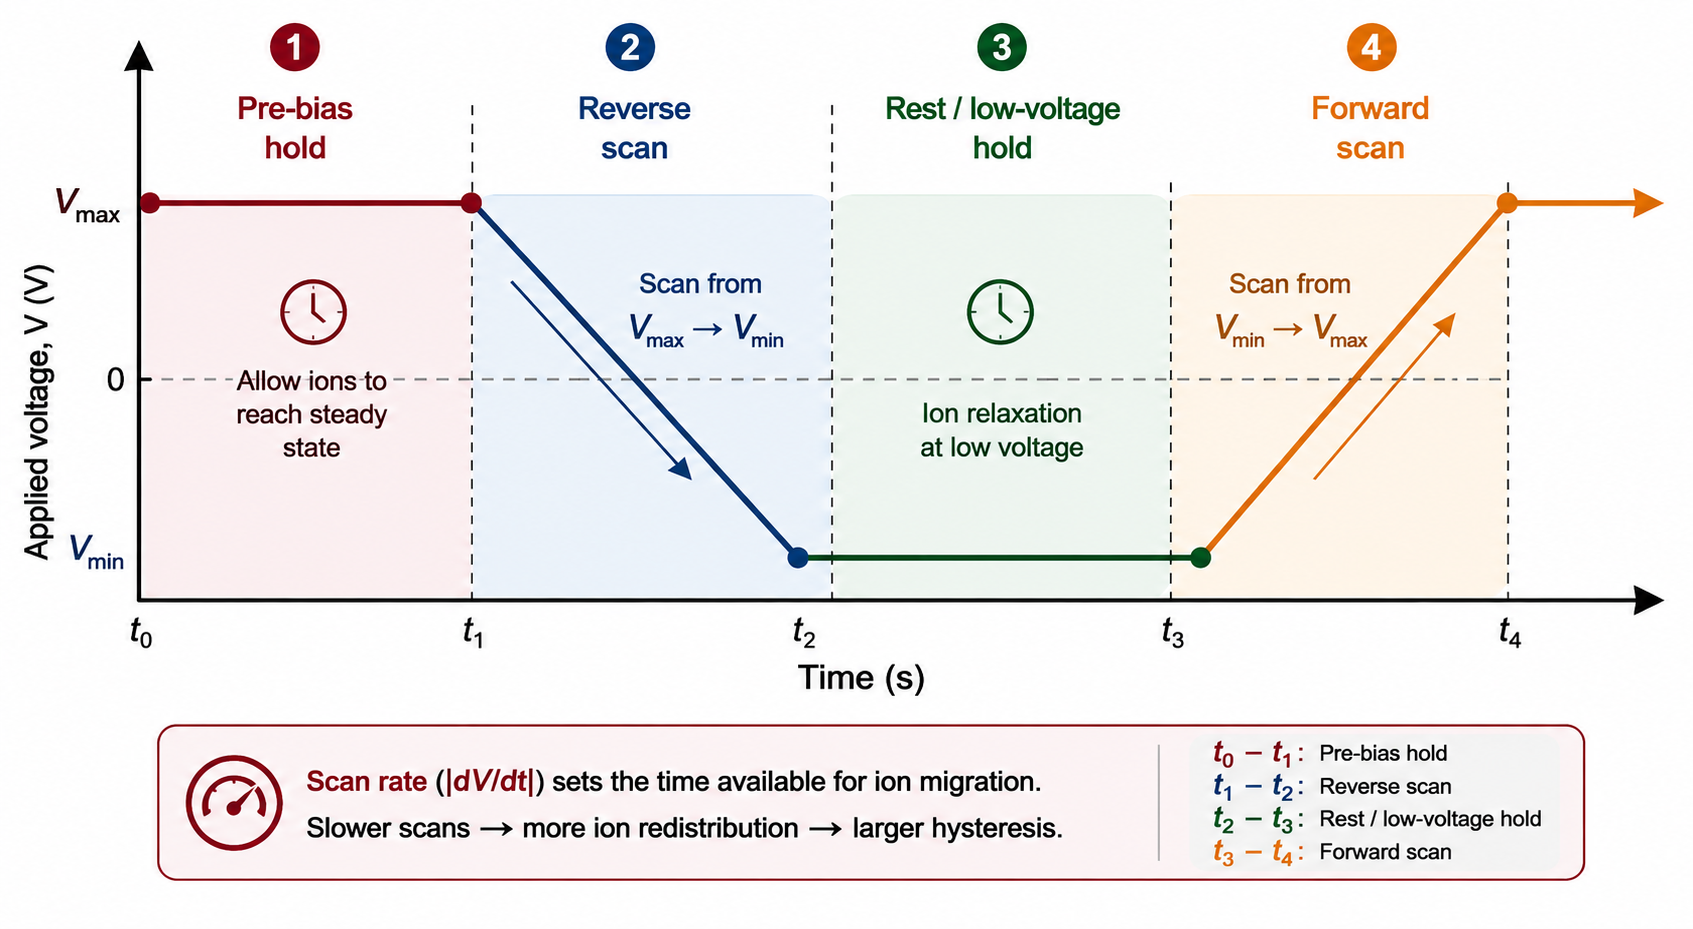
\includegraphics[width=\textwidth]{figures/pptx_ai/jv_scan_protocol_graphic.png}
\caption{Time-dependent J--V scan protocol used for hysteresis simulation. The pre-bias hold defines the initial ionic state, the reverse scan and forward scan impose finite scan-rate dynamics, and the low-voltage hold allows partial ion relaxation before the return sweep.}
\label{fig:voltage_programs}
\end{figure}

The presentation case uses a mobile-ion concentration
\begin{equation}
N_0 = 10^{17}~\mathrm{cm^{-3}},
\end{equation}
ion mobility
\begin{equation}
\mu_{\mathrm{ion}} = 10^{-18}~\mathrm{m^2/(V\,s)},
\end{equation}
and scan rate
\begin{equation}
r_{\mathrm{scan}}=0.1~\mathrm{V/s}.
\end{equation}
Slower scans allow more ion redistribution during the measurement, which can
increase the separation between forward and reverse scans. The simulated
hysteresis result shows that mobile-ion redistribution modifies the internal
field during measurement. It does not yet prove that the chosen ion mobility,
ion concentration, or ion--trap coupling is experimentally unique.

\begin{figure}[H]
\centering
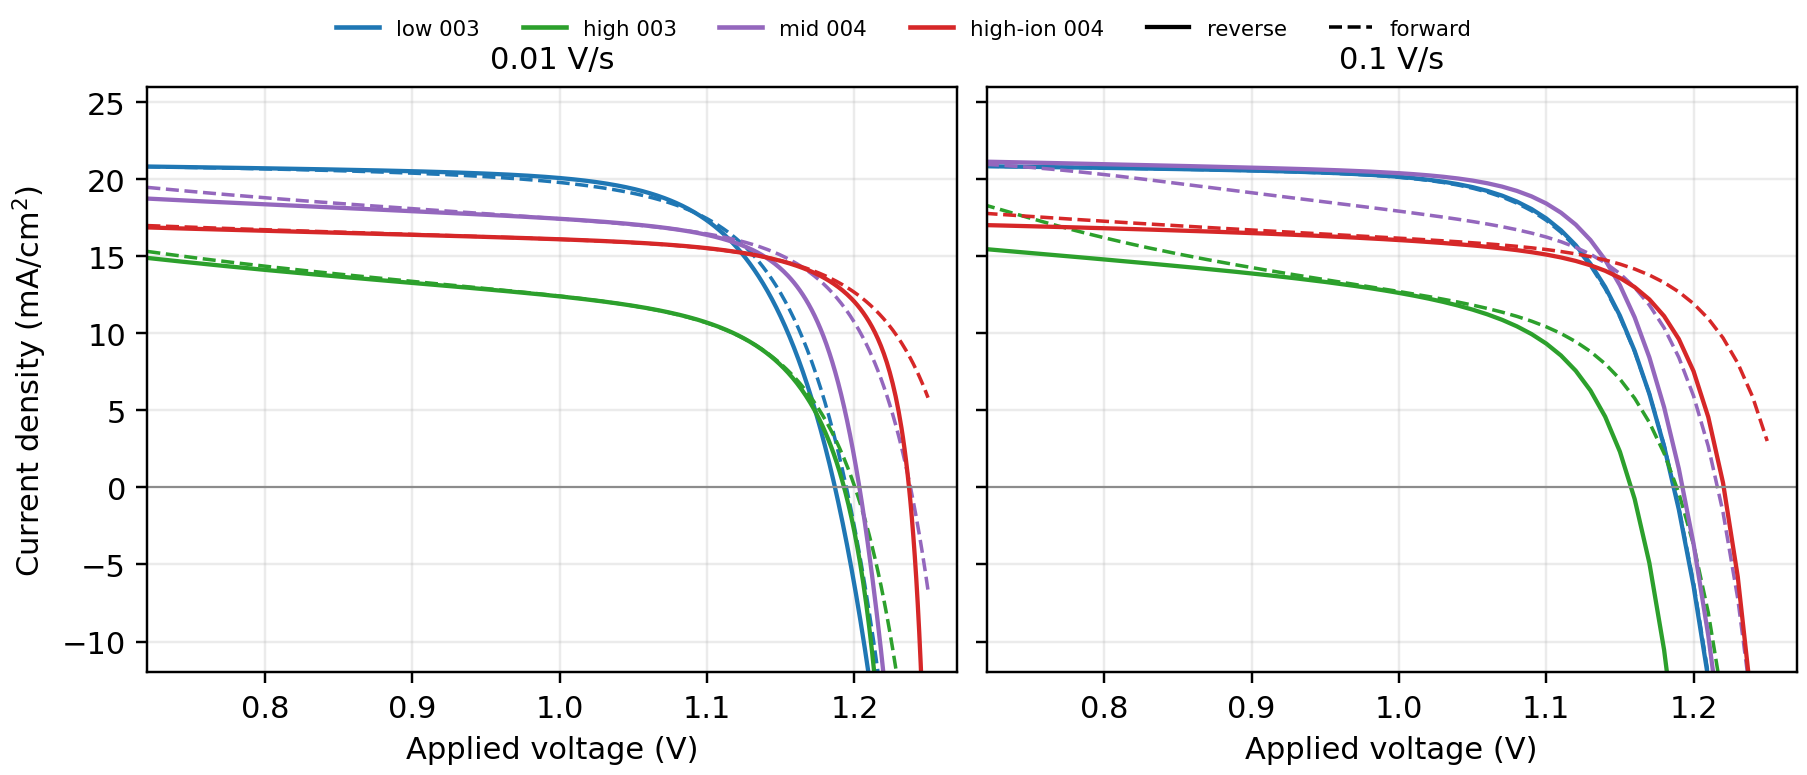
\includegraphics[width=0.78\textwidth]{figures/eee598_comsol/jv_curves.png}
\caption{Representative forward and reverse J--V scans from the multi-rate COMSOL hysteresis study. The scan-direction dependence indicates that the internal electrostatic state changes during the measurement.}
\label{fig:hysteretic_jv}
\end{figure}

\section{DIT Pulse and Mobile-Ion Concentration Extraction}

The drift-ion transient (DIT) protocol provides an ion-sensitive complement to
multi-rate J--V scans. A preconditioned ionic profile is perturbed with a short
voltage pulse, the terminal current transient is recorded, and the mobile-ion
charge associated with the transient component is integrated
\cite{Futscher_2019,SchmidtPRX_2025,SchmidtACS_2025}. In COMSOL, the protocol
is implemented as a time-dependent voltage boundary condition:
\begin{equation}
V_{\mathrm{DIT}}(t)=
\begin{cases}
V_{\mathrm{base}}, & t<t_{\mathrm{on}},\\
V_{oc}, & t_{\mathrm{on}}\le t<t_{\mathrm{off}},\\
V_{\mathrm{base}}, & t\ge t_{\mathrm{off}},
\end{cases}
\qquad
t_{\mathrm{off}}=t_{\mathrm{on}}+10~\mathrm{ms}.
\label{eq:dit_pulse}
\end{equation}
The pulse function belongs only in the time-dependent study. Stationary
initialization and preconditioning studies use constant voltages because the
stationary solver has no time variable and cannot evaluate a function that
depends on \texttt{t}. The DIT study is initialized from the preconditioned
$u_{\mathrm{ion}}(x,0)$ profile and then applies $V_{\mathrm{DIT}}(t)$ to the
terminal or external-circuit boundary.

\begin{figure}[H]
\centering
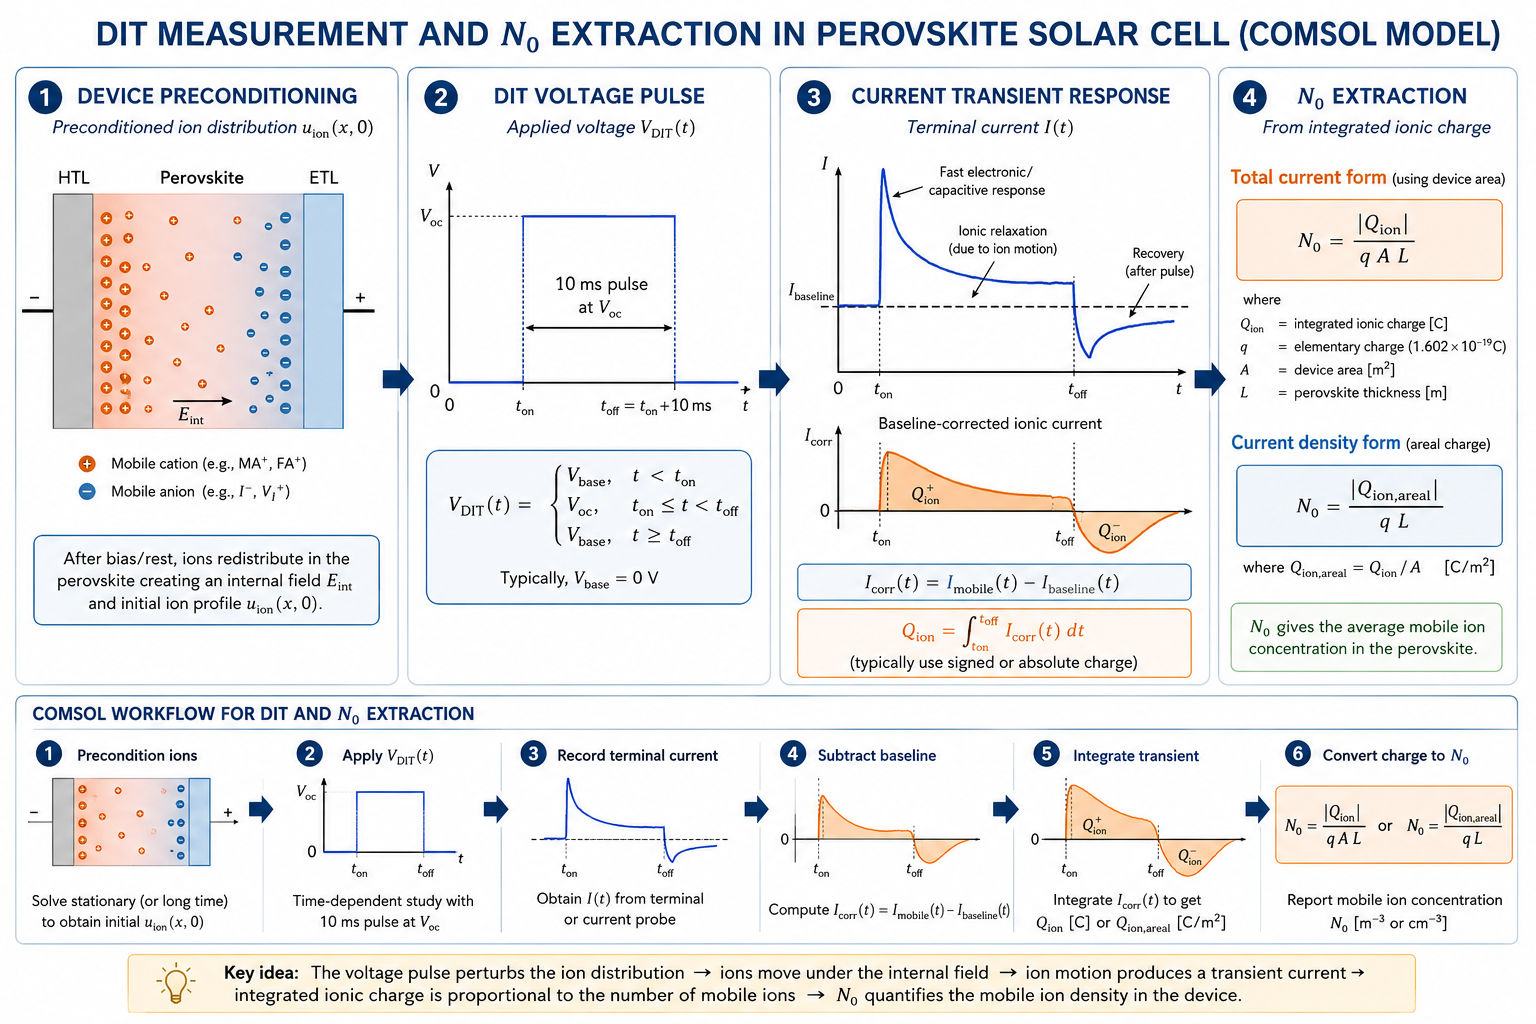
\includegraphics[width=\textwidth]{figures/dit_n0_extraction_infographic.png}
\caption{DIT measurement concept and COMSOL extraction workflow. A preconditioned ion profile is perturbed by a 10 ms voltage pulse, the baseline-corrected current transient is integrated, and the integrated ionic charge is converted into an average mobile-ion concentration.}
\label{fig:dit_n0_extraction}
\end{figure}

The recorded terminal current contains fast electronic, capacitive, leakage,
and ionic contributions. The ion-sensitive quantity is therefore not the raw
current plateau but a baseline-corrected transient:
\begin{equation}
I_{\mathrm{corr}}(t)
=I_{\mathrm{mobile}}(t)-I_{\mathrm{baseline}}(t).
\end{equation}
The best baseline is obtained from an otherwise identical frozen-ion or
ion-blocked control. If only the mobile-ion simulation is available, subtracting
a steady pulse plateau gives an apparent transient charge rather than a unique
mobile-ion density. For total current, the integrated ionic charge and average
mobile-ion concentration are
\begin{align}
Q_{\mathrm{ion}} &=\int_{t_{\mathrm{on}}}^{t_{\mathrm{off}}}
I_{\mathrm{corr}}(t)\,dt,\\
N_0 &=\frac{|Q_{\mathrm{ion}}|}{qAL},
\end{align}
where $A$ is device area and $L$ is perovskite thickness. For current density,
the areal charge form is
\begin{align}
Q_{\mathrm{ion,areal}} &=\int_{t_{\mathrm{on}}}^{t_{\mathrm{off}}}
J_{\mathrm{corr}}(t)\,dt,\\
N_0 &=\frac{|Q_{\mathrm{ion,areal}}|}{qL}.
\end{align}
The sign of $Q_{\mathrm{ion}}$ identifies the transient direction; the
concentration extraction uses the absolute charge magnitude.

A representative 10 ms pulse integrated directly from a terminal-current
trace gives $Q_{\mathrm{ion,areal}}\approx163~\mu\mathrm{C/cm^2}$. For
$L=500$ nm, this corresponds to an apparent upper-bound concentration of about
$2.0\times10^{19}$ cm$^{-3}$. This value is not treated as calibrated because
the full terminal current includes non-ionic plateau and capacitive
contributions. Baseline subtraction of the excess transient is expected to
reduce the extracted concentration substantially, often toward the
$10^{16}$--$10^{17}$ cm$^{-3}$ range for the same film thickness when the
integrated charge is isolated to the ionic relaxation component. The COMSOL
DIT workflow is therefore used as a calibration target for the ion equation,
not as a standalone proof of a unique $N_0$.

\section{Protocol and State Separation}

The voltage protocol preserves scan-rate, bias-history, and hysteresis
information that can be linked to hidden device states. The model therefore
distinguishes controlled inputs,
\begin{equation}
\mathbf{u}(t)=
\left[V_{\mathrm{app}}(t), V_{\mathrm{stress}}(t),
r_{\mathrm{scan}}, t_{\mathrm{pre}}, t_{\mathrm{rest}}\right],
\end{equation}
from internal states,
\begin{equation}
\mathbf{x}(t)=
\left[u_{\mathrm{ion}}(x,t), D_{\mathrm{trap}}(x,t),
D_{Rs}(t), D_{Rsh}(t), D_{\mathrm{cond}}(t)\right].
\end{equation}
This separation prevents scan rate or pre-bias from being misinterpreted as a
material property. It also gives the COMSOL model a practical route to
calibration: the measured voltage program is known, while the internal states
are adjusted only within physically justified parameter ranges.

\chapter{Degradation-State Mappings}

Slow degradation is implemented through bounded damage states rather than by
directly forcing the J--V curve to decay. These states map to model parameters
such as trap density, contact resistance, shunt resistance, surface
recombination, and generation loss, allowing each mechanism to be tested before
the mechanisms are combined.

\section{Purpose of Damage-State Variables}

The COMSOL model uses damage-state variables to connect slow physical changes
to parameters that the Semiconductor Module and Electrical Circuit interface can
use. Each state is dimensionless and bounded. A value of 0 represents the
baseline condition for that mechanism, and a value of 1 represents the selected
maximum severity for the simulated study. The bounded form prevents a numerical
damage variable from growing without physical interpretation.

The model maps latent degradation states onto COMSOL-accessible parameters such
as trap density, ionic charge, series resistance, shunt resistance, surface
recombination, and photogeneration. These mappings are not a substitute for
calibration. They define testable hypotheses about which physical mechanism
produces which J--V signature.

\section{Trap Degradation State}

Trap growth is motivated by defect formation, interfacial disorder, ion-driven
chemical change, and absorber damage. The model can represent trap degradation
either as a spatial PDE $D_{\mathrm{trap}}(x,t)$ in the perovskite domain or as
a lumped global ODE when spatial resolution is not identifiable. The spatial
form is
\begin{equation}
\frac{\partial D_{\mathrm{trap}}}{\partial t}
= k_{\mathrm{trap}} f_{\mathrm{stress}} f_{\mathrm{ion}}
\left(1-D_{\mathrm{trap}}\right)
- k_{\mathrm{heal}} f_{\mathrm{rest}}D_{\mathrm{trap}}.
\label{eq:dtrap}
\end{equation}
The dependent variable is dimensionless, so the source terms must have units of
1/s. The rate constant $k_{\mathrm{trap}}$ has units of 1/s when
$f_{\mathrm{stress}}$ and $f_{\mathrm{ion}}$ are dimensionless multipliers.
The healing term is optional and is used only when recovery during rest is
being tested.

The trap state maps to an effective trap density through either a bounded
linear interpolation,
\begin{equation}
N_{t,\mathrm{eff}} =
N_{t0} + (N_{t,\max}-N_{t0})D_{\mathrm{trap}},
\label{eq:nt_linear}
\end{equation}
or a multiplicative form,
\begin{equation}
N_{t,\mathrm{eff}} =
N_{t0}\left(1+a_{Nt}D_{\mathrm{trap}}\right).
\label{eq:nt_mult}
\end{equation}
Both forms preserve units of m$^{-3}$ or cm$^{-3}$ depending on the COMSOL
parameter convention. The parameter $N_{t,\max}$, or equivalently $a_{Nt}$,
sets the physical severity. A saturated damage state at
$D_{\mathrm{trap}}=1$ therefore means that the selected maximum trap density
has been reached, not that the material contains every possible defect.

In the J--V response, increased $N_t$ shortens SRH lifetimes, increases
nonradiative recombination, lowers $V_{oc}$, and can reduce FF or $J_{sc}$ if
carrier collection becomes recombination-limited. The spatial form can localize
trap growth near interfaces where $u_{\mathrm{ion}}$ or
$\nabla u_{\mathrm{ion}}$ is large. The limitation is that the ion--trap
coupling function $f_{\mathrm{ion}}$ is not unique from J--V data alone and
requires calibration with ion-sensitive or defect-sensitive measurements.

\section{SRH Recombination Coupling}

The SRH recombination expression connects the trap mapping to electronic
transport:
\begin{equation}
R_{\mathrm{SRH}} =
\frac{np-n_i^2}
{\tau_p(n+n_1)+\tau_n(p+p_1)}.
\end{equation}
The lifetimes are
\begin{align}
\tau_n &= \frac{1}{\sigma_n v_{\mathrm{th}} N_{t,\mathrm{eff}}},\\
\tau_p &= \frac{1}{\sigma_p v_{\mathrm{th}} N_{t,\mathrm{eff}}}.
\end{align}
The units are consistent because $\sigma$ has units of m$^2$,
$v_{\mathrm{th}}$ has units of m/s, and $N_t$ has units of m$^{-3}$, so
$\sigma v_{\mathrm{th}}N_t$ has units of 1/s. As
$N_{t,\mathrm{eff}}$ increases, both lifetimes decrease and
$R_{\mathrm{SRH}}$ increases for a given carrier population. This is the
physical path from trap degradation to lower voltage and stronger nonradiative
loss.

\section{Contact Resistance}

Contact resistance represents voltage loss at the metal or transport-layer
contact. In this model it is associated with the rear Ag contact boundary or an
equivalent circuit element. The area-normalized form is
\begin{equation}
V_{\mathrm{terminal}} =
V_{\mathrm{device}} + J R_{s,A},
\label{eq:rs_area}
\end{equation}
where $J$ is current density and $R_{s,A}$ has units of $\Omega\,\mathrm{m^2}$.
If a total current $I$ and device area $A$ are used instead, the equivalent
relation is
\begin{equation}
V_{\mathrm{terminal}} =
V_{\mathrm{device}} + J A R_s.
\end{equation}

The degradation mapping is
\begin{equation}
R_{s,\mathrm{eff}} =
R_{s0}\left(1+a_{Rs}D_{Rs}\right).
\label{eq:rs_deg}
\end{equation}
Increasing $R_s$ primarily rounds the high-forward-bias J--V knee and lowers
fill factor. It has little direct effect on $V_{oc}$ because the terminal
current is near zero at open circuit. The COMSOL interpretation is lumped
contact or interfacial voltage loss, not a spatially resolved chemical reaction
at the Ag boundary.

If light-soaking or contact activation is included, conditioning can reduce the
effective series resistance:
\begin{equation}
R_{s,\mathrm{eff}} =
\frac{R_{s0}\left(1+a_{Rs}D_{Rs}\right)}
{1+a_{\mathrm{cond}}D_{\mathrm{cond}}}.
\label{eq:rs_cond}
\end{equation}
The denominator represents beneficial extraction or contact activation. This
term is proposed for future calibration and is not treated as validated in the
present results.

\section{Shunt Resistance}

Shunting is represented as a leakage pathway in parallel with the photovoltaic
device. In area-normalized form,
\begin{equation}
J_{\mathrm{sh}} = \frac{V}{R_{sh,A}},
\label{eq:jsh}
\end{equation}
where $R_{sh,A}$ has units of $\Omega\,\mathrm{m^2}$. Equivalently, the model
can use a shunt conductance
\begin{equation}
G_{sh,\mathrm{eff}}=
G_{sh0}+\Delta G_{sh}D_{Rsh}.
\end{equation}
The resistance mapping can be written as
\begin{equation}
R_{sh,\mathrm{eff}} =
\frac{R_{sh0}}{1+a_{Rsh}D_{Rsh}}.
\label{eq:rsh_deg}
\end{equation}

Decreasing $R_{sh}$ increases leakage current near short circuit and changes
the low-voltage slope of the J--V curve. The usual signatures are FF loss and,
when leakage is strong enough, reduced $V_{oc}$. Because this effect is
introduced through a circuit-equivalent pathway, it is interpreted as lumped
leakage rather than a spatially resolved pinhole or defect filament.

\section{Surface Recombination and Photogeneration Loss}

Surface recombination is represented by an interface recombination velocity
$S$, with units of m/s. Increasing $S$ raises interface recombination and can
lower $V_{oc}$ and FF when interface carrier concentrations are high. The
mapping has the same bounded structure:
\begin{equation}
S_{\mathrm{eff}}=S_0\left(1+a_S D_S\right).
\end{equation}
The limitation is observability: terminal J--V data may not separate surface
recombination from bulk trap recombination without additional observables.

Photogeneration loss can be represented by reducing the absorber generation
rate:
\begin{equation}
G_{\mathrm{eff}}=G_0\left(1-a_GD_G\right).
\end{equation}
This mapping tests absorber damage or optical loss. Its primary J--V signature
is reduced $J_{sc}$, with secondary effects on PCE and possibly FF. It should
not be used to represent recombination loss unless
independent optical or quantum-efficiency evidence supports that choice.

\section{Light Soaking and Self-Healing}

PSCs can show beneficial conditioning under illumination and partial recovery
after rest. Light soaking can improve extraction or contact behavior, often
appearing as higher FF and sometimes higher PCE. Self-healing can occur through
ion redistribution, trap relaxation, and contact or interfacial
re-equilibration after stress is removed.

A proposed conditioning state is
\begin{equation}
\frac{dD_{\mathrm{cond}}}{dt}
= k_{\mathrm{cond}}f_{\mathrm{light}}f_T
\left(1-D_{\mathrm{cond}}\right)
- k_{\mathrm{relax}}D_{\mathrm{cond}}.
\label{eq:dcond}
\end{equation}
The state is dimensionless, so $k_{\mathrm{cond}}$ and $k_{\mathrm{relax}}$
have units of 1/s when the multipliers are dimensionless. The proposed mapping
to series resistance is Eq.~\ref{eq:rs_cond}.

Optional trap healing can be represented by the negative term in
Eq.~\ref{eq:dtrap}:
\begin{equation}
\frac{dD_{\mathrm{trap}}}{dt}
= k_{\mathrm{trap}}f_{\mathrm{stress}}
\left(1-D_{\mathrm{trap}}\right)
- k_{\mathrm{heal}}f_{\mathrm{rest}}D_{\mathrm{trap}}.
\end{equation}
These terms are physically motivated, but they are not fully validated in the
present COMSOL model. They remain future implementation targets that require
controlled light-soaking and rest-recovery data.

\chapter{Experimental Comparison and Calibration Targets}

\section{Purpose of the Comparison}

The experimental comparison evaluates whether the COMSOL model reproduces the
direction and approximate shape of observed degradation. It is not an absolute
calibration of device performance or field lifetime. The COMSOL degradation
rate was accelerated to reduce computational time, so simulated seconds and
experimental hours are not directly equivalent.

The comparison uses two reference points: a baseline electronic state and a
degraded light-plus-heat state. The interpretation focuses on PCE reduction,
fill-factor loss, J--V shape, and the mechanism balance among trap growth,
shunting, contact resistance, and mobile-ion redistribution.

\section{Baseline Electronic State}

The experimental X12 baseline has
\begin{equation}
\mathrm{PCE}=14.10\%.
\end{equation}
The COMSOL baseline has
\begin{equation}
\mathrm{PCE}=20.24\%, \qquad
V_{oc}=1.125~\mathrm{V}, \qquad
\mathrm{FF}=83.27\%, \qquad
J_{sc}=21.61~\mathrm{mA/cm^2}.
\end{equation}
The COMSOL baseline is more ideal than the experiment. This mismatch is
expected for an initial physics model because idealized contacts, uniform
or simplified photogeneration, one-dimensional geometry, and literature-based material
parameters tend to reduce nonradiative and resistive losses. The baseline
therefore provides a reference for mechanism studies, not a fully calibrated
absolute representation of the experimental device.

The calibration target is clear: absolute baseline performance requires
adjusting absorber generation, transport-layer barriers, trap density, surface
recombination, contact resistance, and shunt leakage so that $V_{oc}$,
$J_{sc}$, FF, and PCE all match the same device before degradation parameters
are interpreted physically.

\section{Degraded Light-Plus-Heat State}

The experimental device after 24 h light-plus-heat stress has
\begin{equation}
\mathrm{PCE}=10.05\%.
\end{equation}
The accelerated COMSOL light-plus-heat case after 60 s has
\begin{equation}
\mathrm{PCE}=10.85\%, \qquad
V_{oc}=1.021~\mathrm{V}, \qquad
\mathrm{FF}=53.46\%, \qquad
J_{sc}=19.87~\mathrm{mA/cm^2}.
\end{equation}
The simulated degradation direction is consistent with the experimental trend:
PCE decreases, FF decreases strongly, and the J--V curve develops a degraded
knee. The simulated $J_{sc}$ also decreases, which is consistent with stronger
recombination or reduced effective generation.

The agreement is qualitative. The comparison supports the use of trap growth,
shunt leakage, contact resistance, and mobile-ion redistribution as candidate
mechanisms, but it does not uniquely identify their relative weights. The
accelerated timescale, baseline mismatch, and incomplete validation of
ion--trap coupling prevent a calibrated lifetime claim.

\section{Stress-Specific Comparison Targets}

The Research Explorer comparison package adds stress-specific experimental
targets for light-only, heat-only, and light-plus-heat exposure. These figures
combine experimental metric scatter, median trends, and representative J--V
curves with the current COMSOL comparison cases. They are used here as
calibration targets rather than as fitted validation, because the experimental
sets differ in stress duration, light intensity, sample count, and starting
device performance.

\begin{figure}[H]
\centering
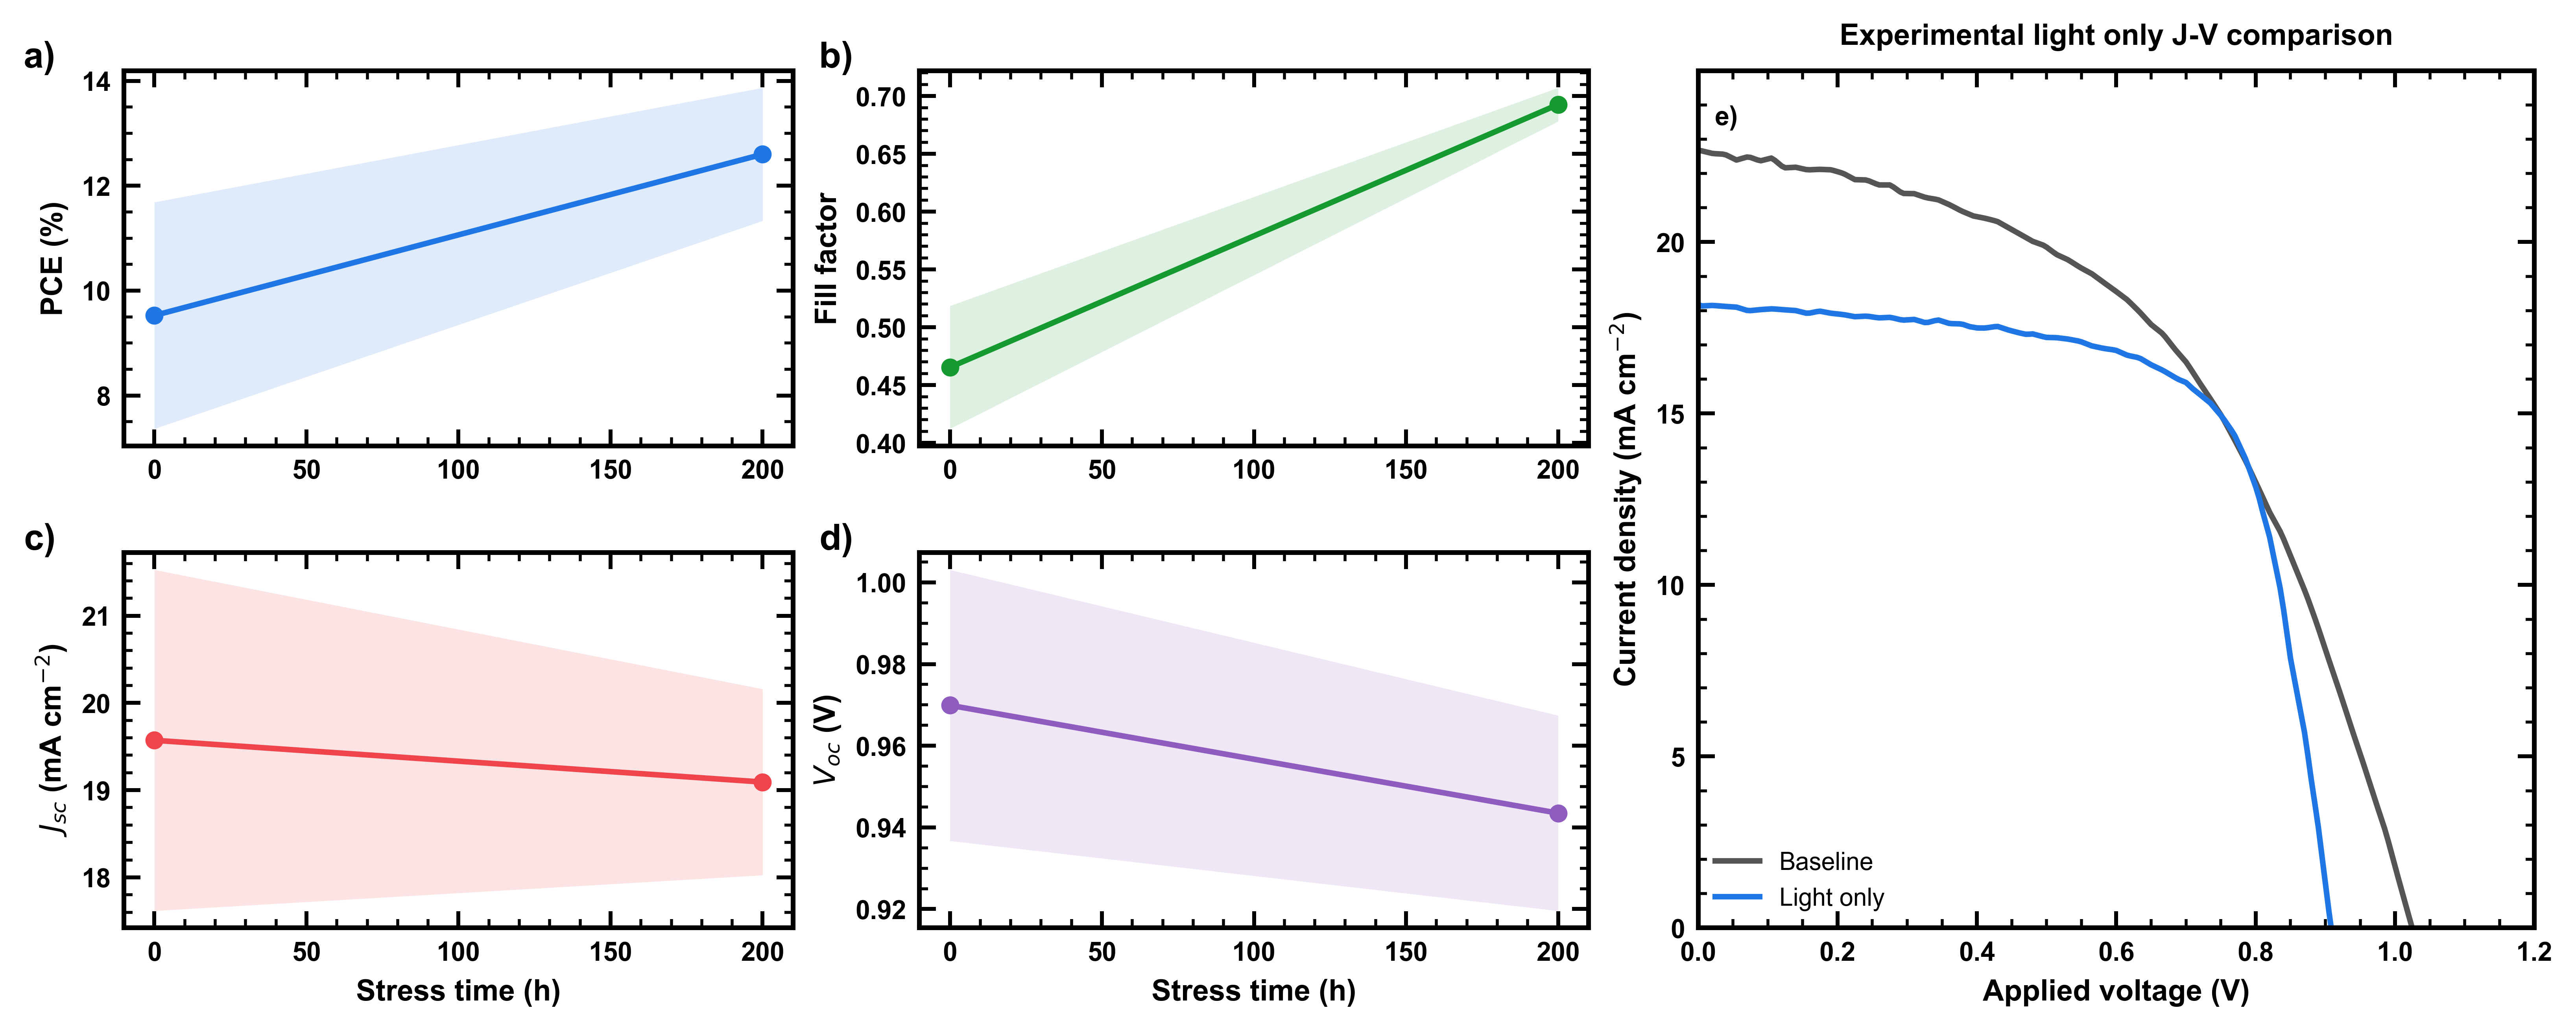
\includegraphics[width=\textwidth]{outputs/figures/comsol_experimental_comparison/xrf_light_only_comsol_comparison.png}
\caption{Light-only experimental comparison used as a COMSOL calibration
target. The light-only endpoint shows a much milder degradation signature than
the coupled light-plus-heat case, so light-driven trap and transport changes
should remain weaker than the combined stress channel.}
\label{fig:xrf_light_only_comsol_comparison}
\end{figure}

\begin{figure}[H]
\centering
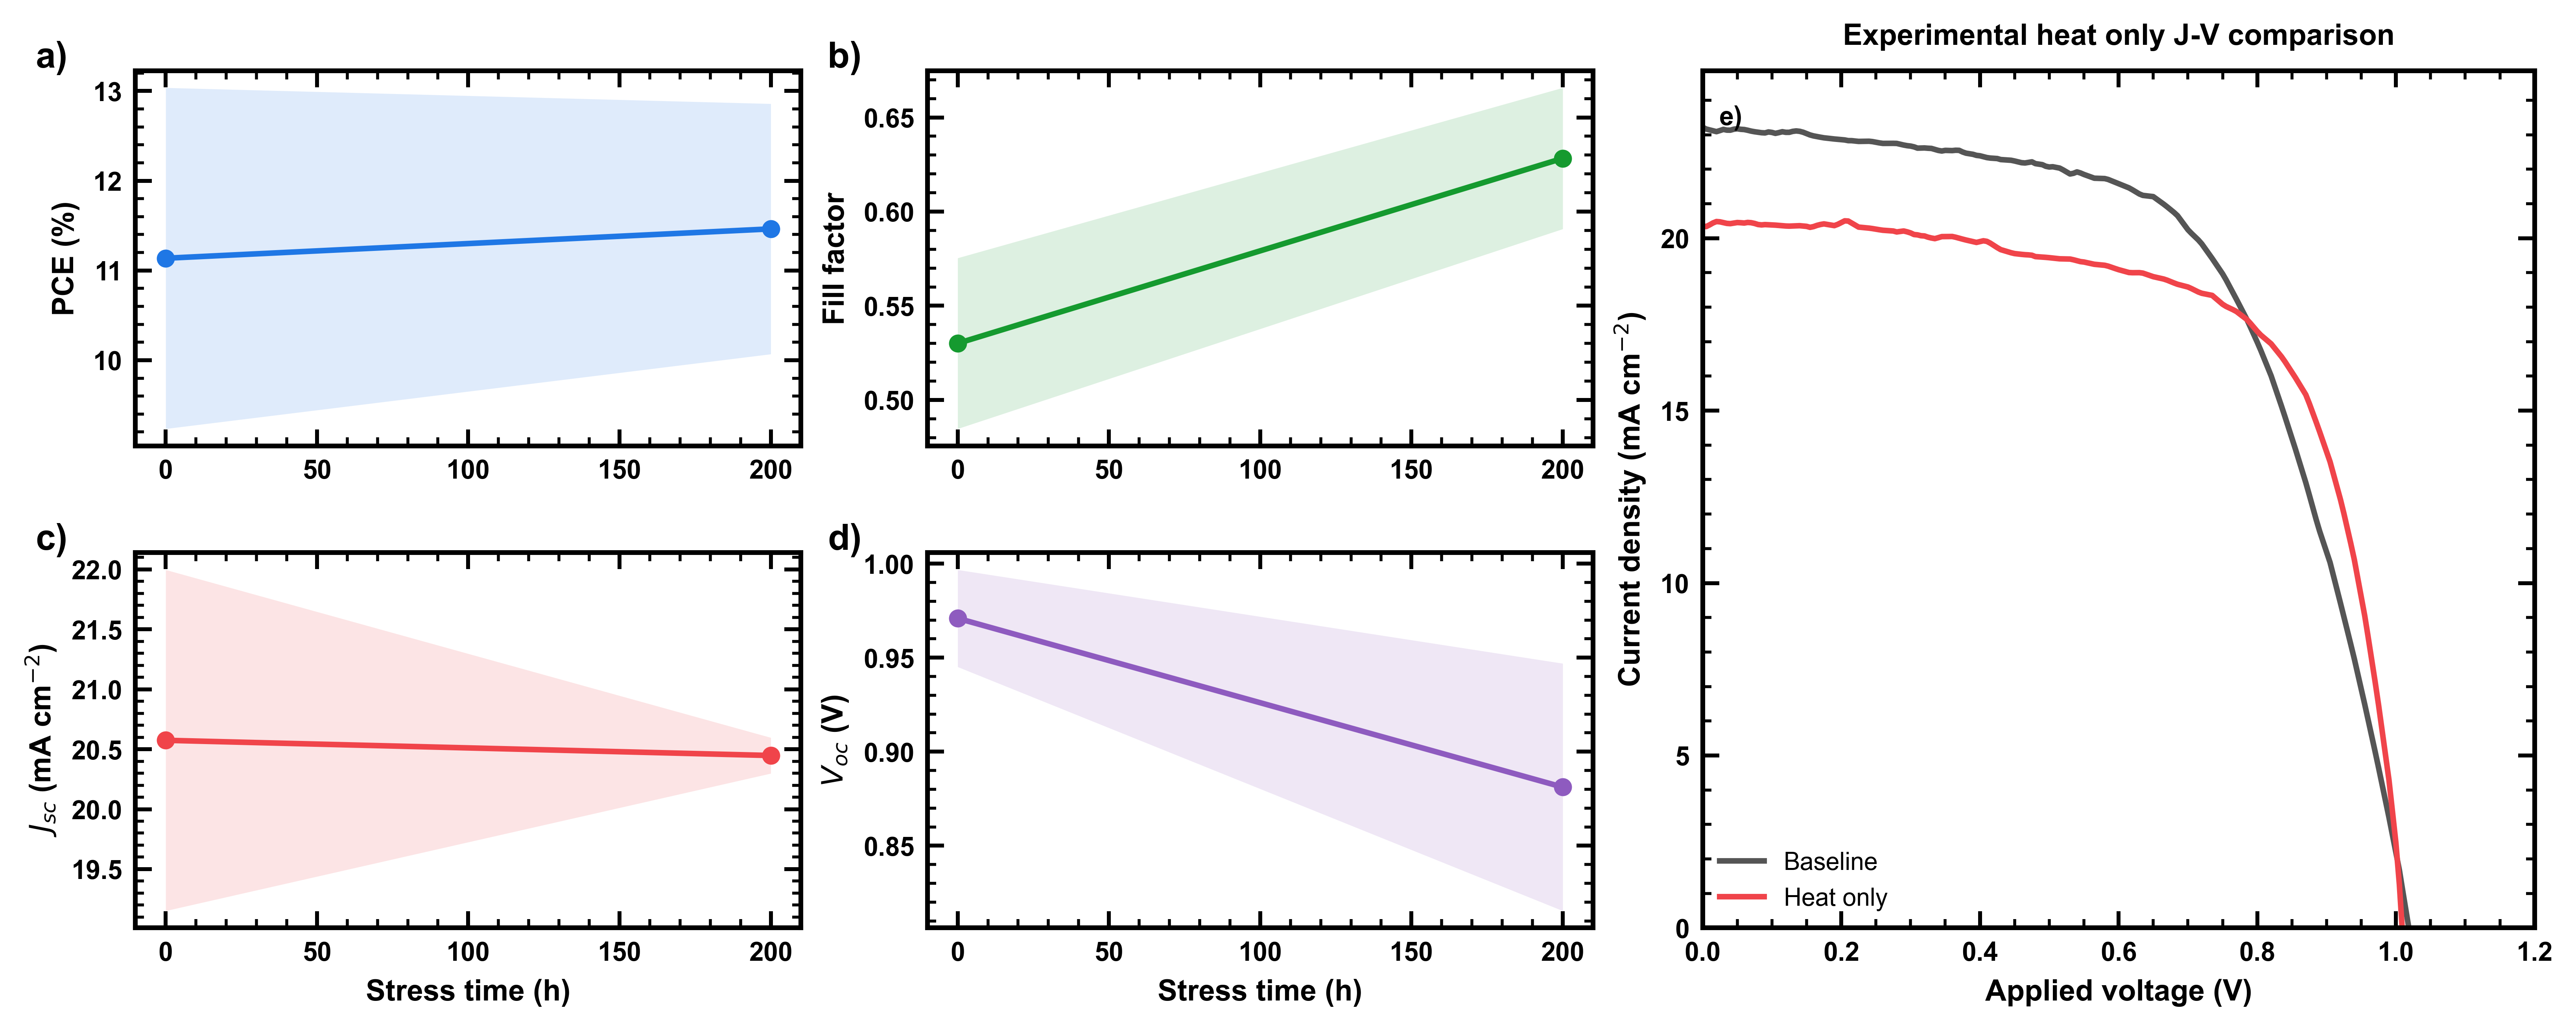
\includegraphics[width=\textwidth]{outputs/figures/comsol_experimental_comparison/xrf_heat_only_comsol_comparison.png}
\caption{Heat-only experimental comparison used as a COMSOL calibration
target. This case isolates the thermal contribution and constrains the model so
that heat by itself does not reproduce the full coupled light-plus-heat
degradation pathway.}
\label{fig:xrf_heat_only_comsol_comparison}
\end{figure}

\begin{figure}[H]
\centering
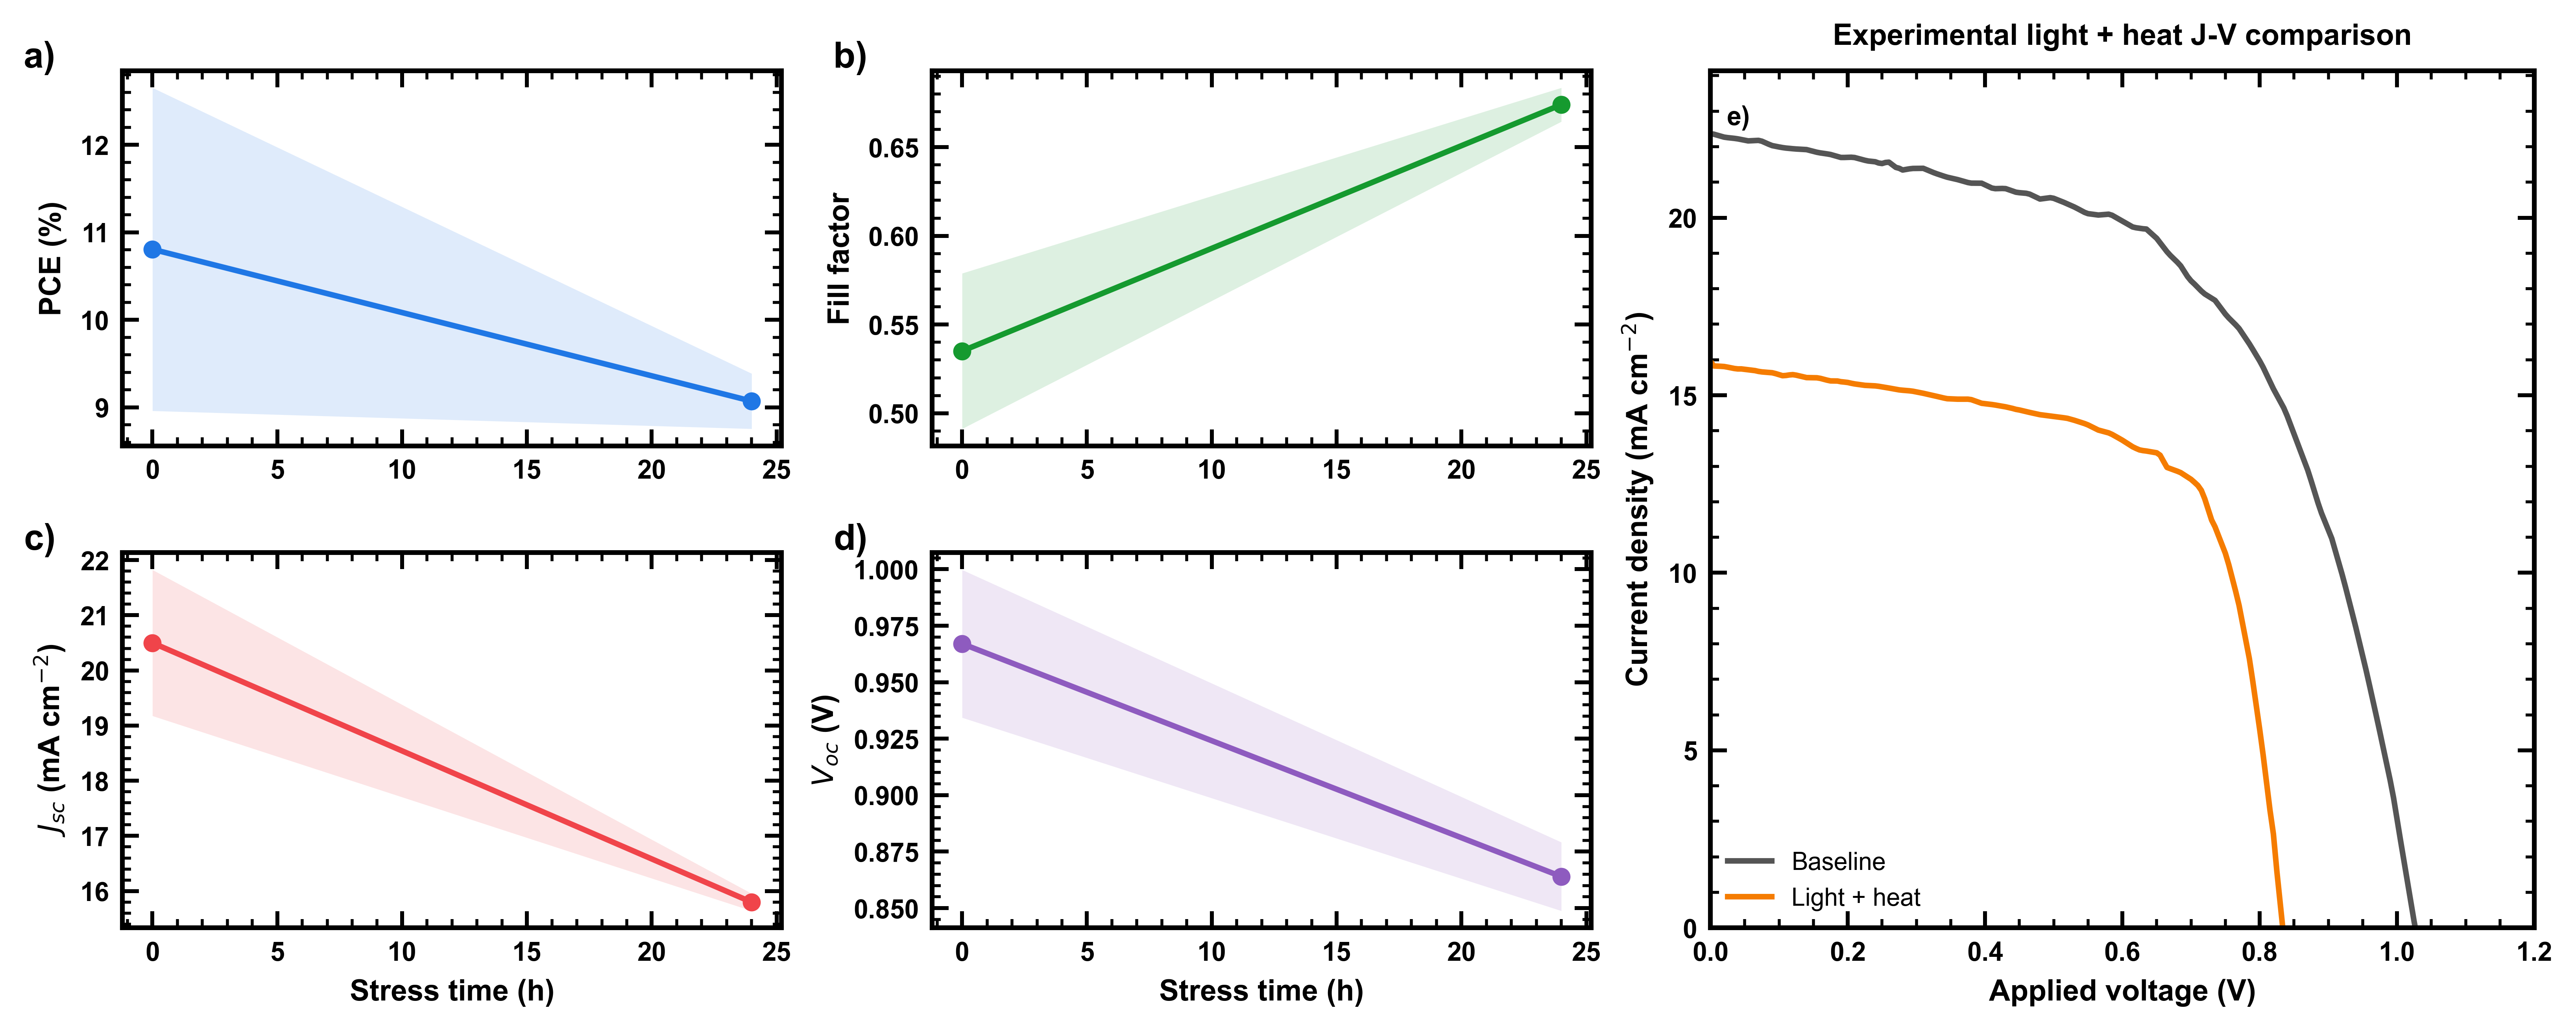
\includegraphics[width=\textwidth]{outputs/figures/comsol_experimental_comparison/xrf_light_heat_comsol_comparison.png}
\caption{Light-plus-heat experimental comparison used as a COMSOL calibration
target. The coupled stress condition produces the strongest endpoint loss in
the matched XRF stress matrix and is therefore the primary target for tuning
combined recombination, transport, and leakage changes.}
\label{fig:xrf_light_heat_comsol_comparison}
\end{figure}

\begin{figure}[H]
\centering
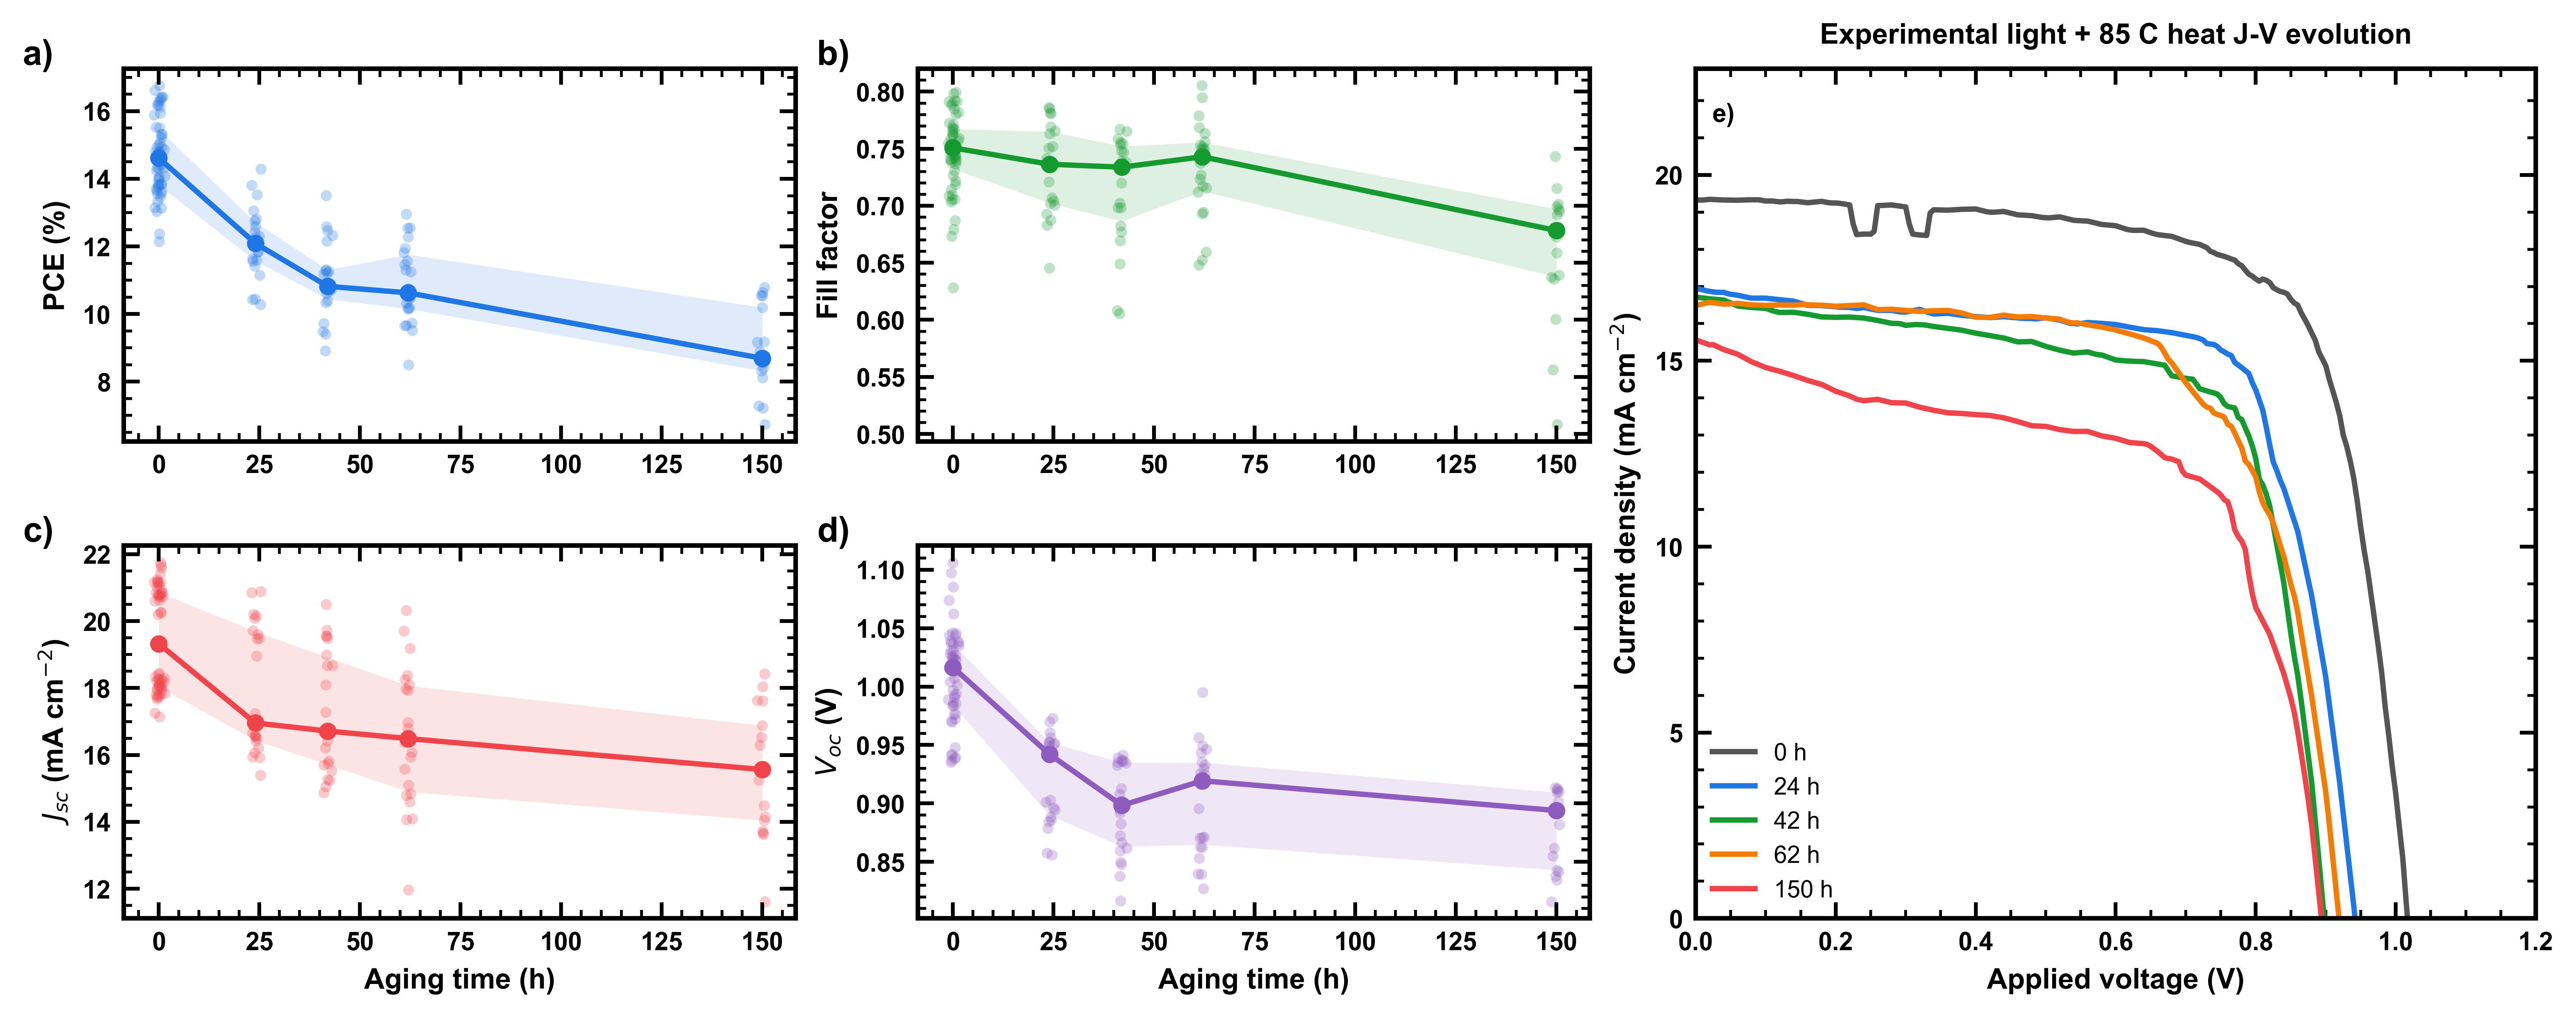
\includegraphics[width=\textwidth]{outputs/figures/comsol_experimental_comparison/exp3_lh_85c_comsol_comparison.png}
\caption{Light plus 85~$^\circ$C aging comparison from the Exp3 dataset. The
larger time series shows sustained performance loss, with median PCE decreasing
from about 14.6\% at 0 h to about 8.7\% at 150 h, and provides the strongest
multi-time-point target for coupled degradation calibration.}
\label{fig:exp3_lh_85c_comsol_comparison}
\end{figure}

Together, these comparisons show why the degradation model should not be
calibrated only to PCE. Light-only and heat-only endpoints show milder or
partially compensating changes in the electronic metrics, while coupled
light-plus-heat exposure produces a more consistent loss in current, voltage,
fill factor, and J--V curve shape. A useful calibration must therefore match
both the metric trajectories and the stress-dependent J--V shape.

\section{Mechanism Balance}

Several mechanisms can produce similar PCE loss. Increased trap density lowers
carrier lifetimes through the SRH relation and reduces $V_{oc}$. Decreased
shunt resistance increases leakage near short circuit and reduces FF. Increased
series resistance rounds the high-forward-bias knee and reduces FF with limited
direct effect on $V_{oc}$. Mobile-ion redistribution changes the internal
space-charge profile through Eq.~\ref{eq:rho_ion}, shifting band bending and
creating scan-history dependence.

The degraded comparison therefore cannot be interpreted from PCE alone. A
calibrated fit must match the full J--V shape, forward/reverse scan separation,
voltage-dependent slope, and time evolution. Impedance, transient photocurrent,
capacitance, photoluminescence, and ion-current measurements would reduce the
non-uniqueness by constraining mobile-ion and recombination parameters
\cite{SchmidtPRX_2025,Elhorst_2025,SchmidtACS_2025}.

\section{Calibration Needs}

The model needs four calibration steps before it can support device-specific
lifetime prediction:
\begin{enumerate}
\item match the pristine J--V curve in absolute $V_{oc}$, $J_{sc}$, FF, and
PCE;
\item calibrate the accelerated degradation factors against measured aging
times;
\item separate the relative contributions of trap loss, shunt loss, contact
resistance, photogeneration loss, and surface recombination; and
\item validate the mobile-ion distribution and ion--trap coupling with
ion-sensitive or hysteresis-sensitive measurements.
\end{enumerate}

Until those steps are complete, the COMSOL model is best interpreted as a
physics-based mechanism-separation platform rather than a final lifetime
prediction tool.

\section{Architecture-Specific Calibration Context}

The laboratory program includes both
ITO-glass/NiO$_x$/perovskite/C$_{60}$/BCP/Ag devices and bilayer
ITO-glass/NiO$_x$/MeO-2PACz/perovskite/C$_{60}$/BCP/Ag devices. The
presentation and this thesis use the bilayer p-i-n architecture as the primary
device truth. Baseline, light-only, heat-only, light-plus-heat, glovebox
control, and dark-recovery measurements should therefore be grouped by
architecture before parameter fitting.

Literature and laboratory comparisons indicate that different absorber and
contact architectures need not degrade through the same dominant electrical
signature. A strong $J_{sc}$ decrease suggests generation or collection loss,
a dominant FF decrease suggests contact or shunt loss, and a large $V_{oc}$
decrease suggests stronger recombination. These are diagnostic hypotheses, not
unique assignments. The model should fit the complete J--V curve and supporting
ion-sensitive or optical measurements before attributing a measured trend to
one channel.

\chapter{Simulation Results and Interpretation}

\section{Data Provenance and Scope}

Chapter~7 intentionally combines several COMSOL export generations because each
one answers a different validation question. The accelerated degradation
baseline is an earlier compact trajectory used to demonstrate coupled aging
behavior. The electronic parameter sweep is a static sensitivity export used to
check the direction and magnitude of terminal J--V responses. The current
canonical light-temperature aging grid is
\path{data/raw/comsol/arch_baseline_pin/Aging/Stress_matrix_jv_003.csv}; it is
the source for the 360-curve stress-matrix results. Earlier stress-matrix J--V
exports are retained only as audit history. Absolute PCE, lifetime, and
hysteresis values should therefore be compared within each section's stated
data source, not across these separate export protocols unless the comparison
is explicitly identified as qualitative.

\section{Accelerated Degradation Baseline}

The processed COMSOL degradation export contains 12 scenarios, 11 aging times,
and 58 voltage points per scenario-time pair. The full coupled accelerated
baseline decreases from 21.35\% PCE at 0 h to 16.51\% PCE at 3000 h. Linear
interpolation of the processed trajectory gives $T_{90}=515$ h and
$T_{80}=2415$ h. These values are model outputs for an accelerated scenario,
not field-lifetime predictions.

\begin{table}[H]
\centering
\caption{Compact summary of the accelerated COMSOL degradation baseline.}
\label{tab:baseline_summary}
\begin{tabular}{@{}ll@{}}
\toprule
Quantity & Processed value \\
\midrule
Scenarios & 12 \\
Aging times & 11 \\
Voltage points per scenario-time pair & 58 \\
Full-case PCE at 0 h & 21.35\% \\
Full-case PCE at 3000 h & 16.51\% \\
Interpolated $T_{90}$ & 515 h \\
Interpolated $T_{80}$ & 2415 h \\
\bottomrule
\end{tabular}
\end{table}

\begin{figure}[H]
\centering
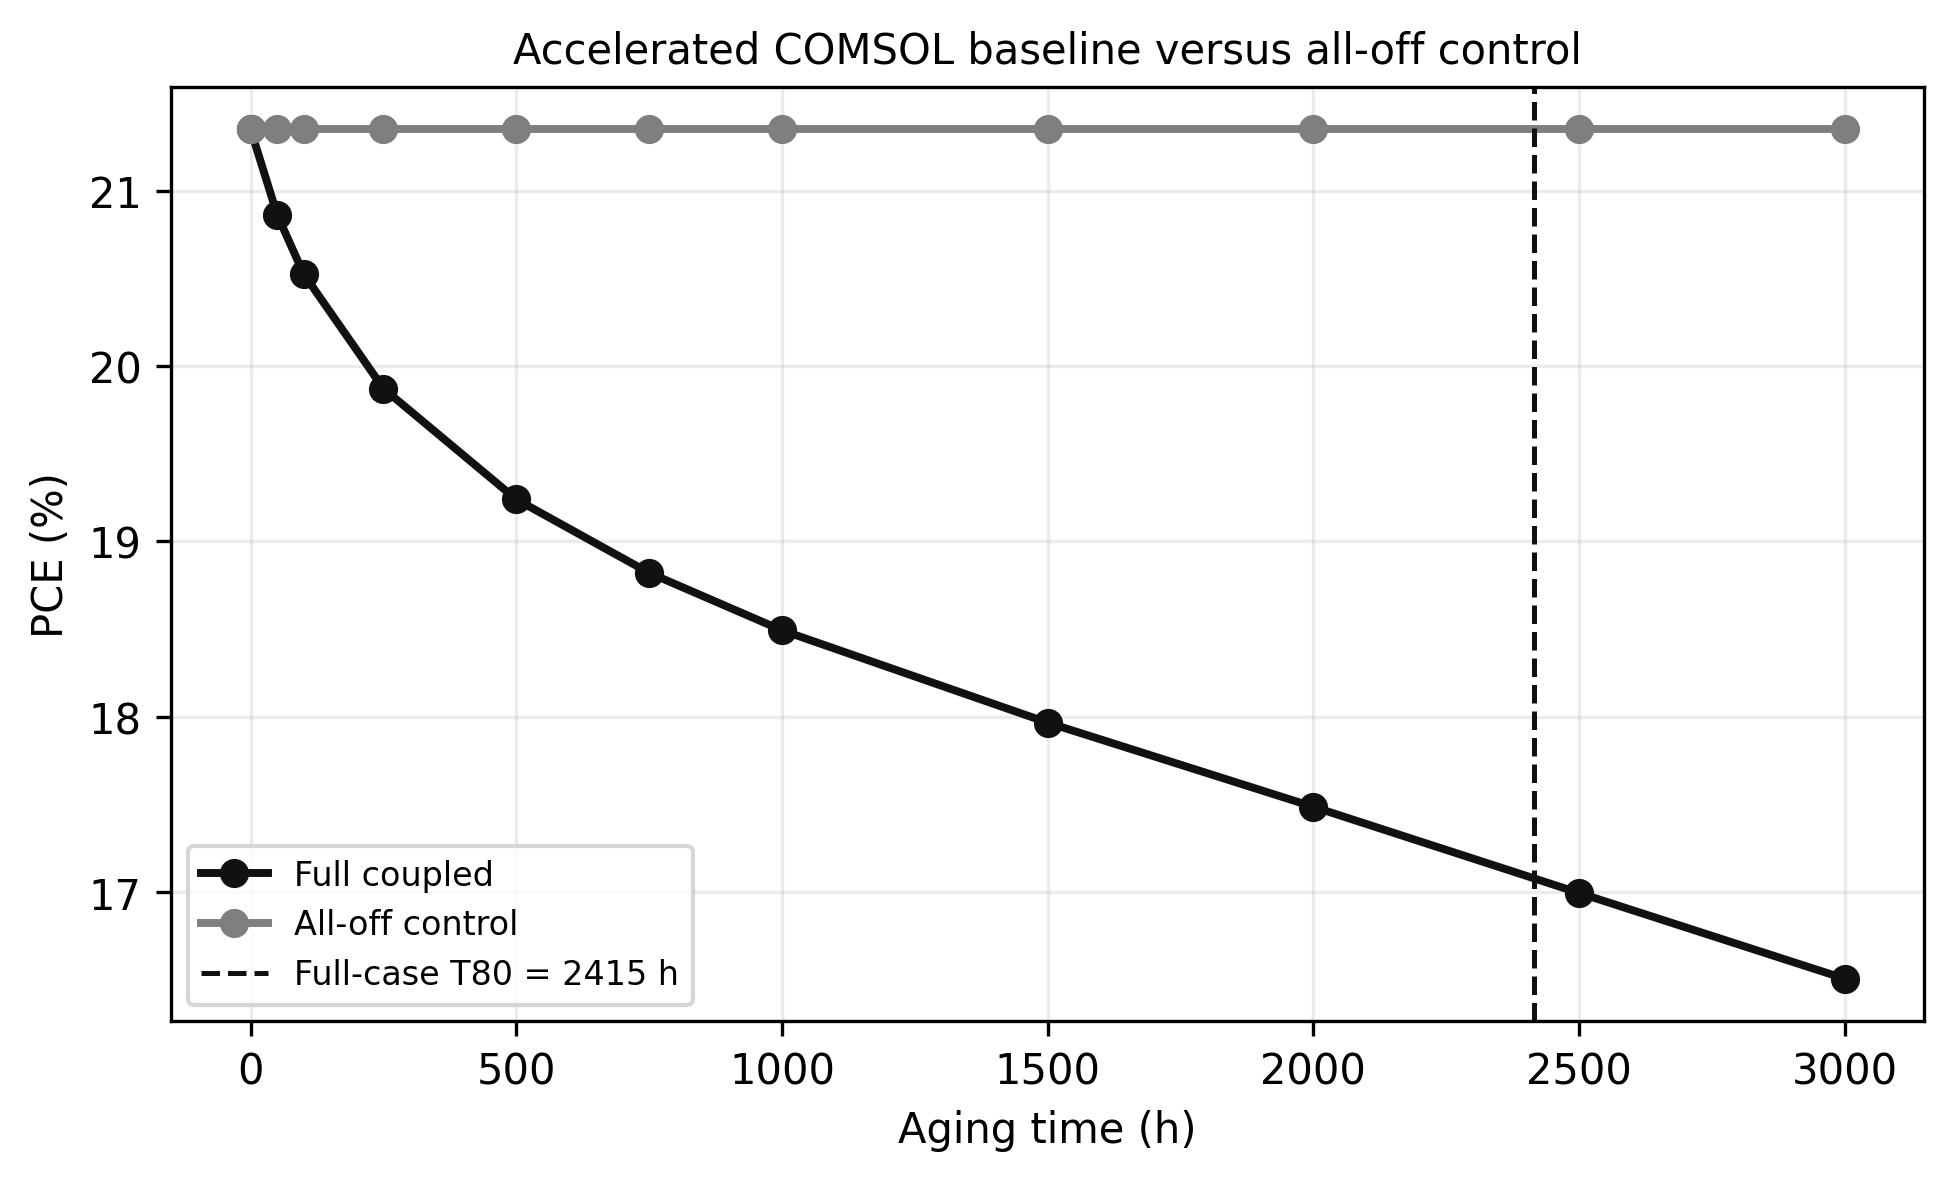
\includegraphics[width=0.82\textwidth]{outputs/figures/comsol_baseline_pce.png}
\caption{COMSOL full coupled degradation baseline compared with the all-off control. The full coupled case reaches interpolated $T_{80}=2415$ h.}
\label{fig:comsol_baseline_pce}
\end{figure}

Figure~\ref{fig:comsol_baseline_pce} shows that the full coupled case loses PCE
while the all-off control remains flat. The variable that changes is the
mechanism-state vector that maps into $N_t$, $R_s$, $R_{sh}$, $Q_f$, and
surface recombination. The equations causing the change are the bounded
degradation mappings described in Chapter~5. Physically, the curve represents
accelerated combined degradation rather than one isolated mechanism. The J--V
signature is a loss in extracted power over aging time. The interpretation is
qualitative until the accelerated degradation amplitudes are calibrated to
matched experimental stress data.

\begin{table}[H]
\centering
\caption{Lifetime summary for the control, full-coupled baseline, and the active one-only and leave-one-out mechanism studies.}
\label{tab:comsol_lifetime_summary}
\small
\begin{tabular}{@{}lrrrrr@{}}
\toprule
scenario & PCE0\_pct & PCE\_3000\_pct & PCE\_retention\_3000 & T90\_h & T80\_h \\
\midrule
full & 21.350 & 16.507 & 0.773 & 515.261 & 2414.671 \\
no Rsh & 21.350 & 18.170 & 0.851 & 601.744 & -- \\
no Nt & 21.350 & 19.698 & 0.923 & -- & -- \\
no Qf & 21.350 & 15.861 & 0.743 & 393.671 & 1768.072 \\
control & 21.350 & 21.350 & 1.000 & -- & -- \\
only Rsh & 21.350 & 19.333 & 0.906 & -- & -- \\
only Nt & 21.350 & 17.444 & 0.817 & 423.679 & -- \\
only Qf & 21.350 & 21.783 & 1.020 & -- & -- \\
\bottomrule
\end{tabular}
\end{table}


Table~\ref{tab:comsol_lifetime_summary} reports the main lifetime markers.
The one-only $N_t$ case produces a large PCE loss but does not cross $T_{80}$
within 3000 h. The one-only $Q_f$ case improves the J--V output in this
parameterization, so removing $Q_f$ from the full coupled case makes
degradation more severe. This counteracting behavior shows why additive
mechanism assumptions should be checked directly in the COMSOL library rather
than assumed to be linear and monotonic.

\section{J--V and State Evolution}

\begin{figure}[H]
\centering
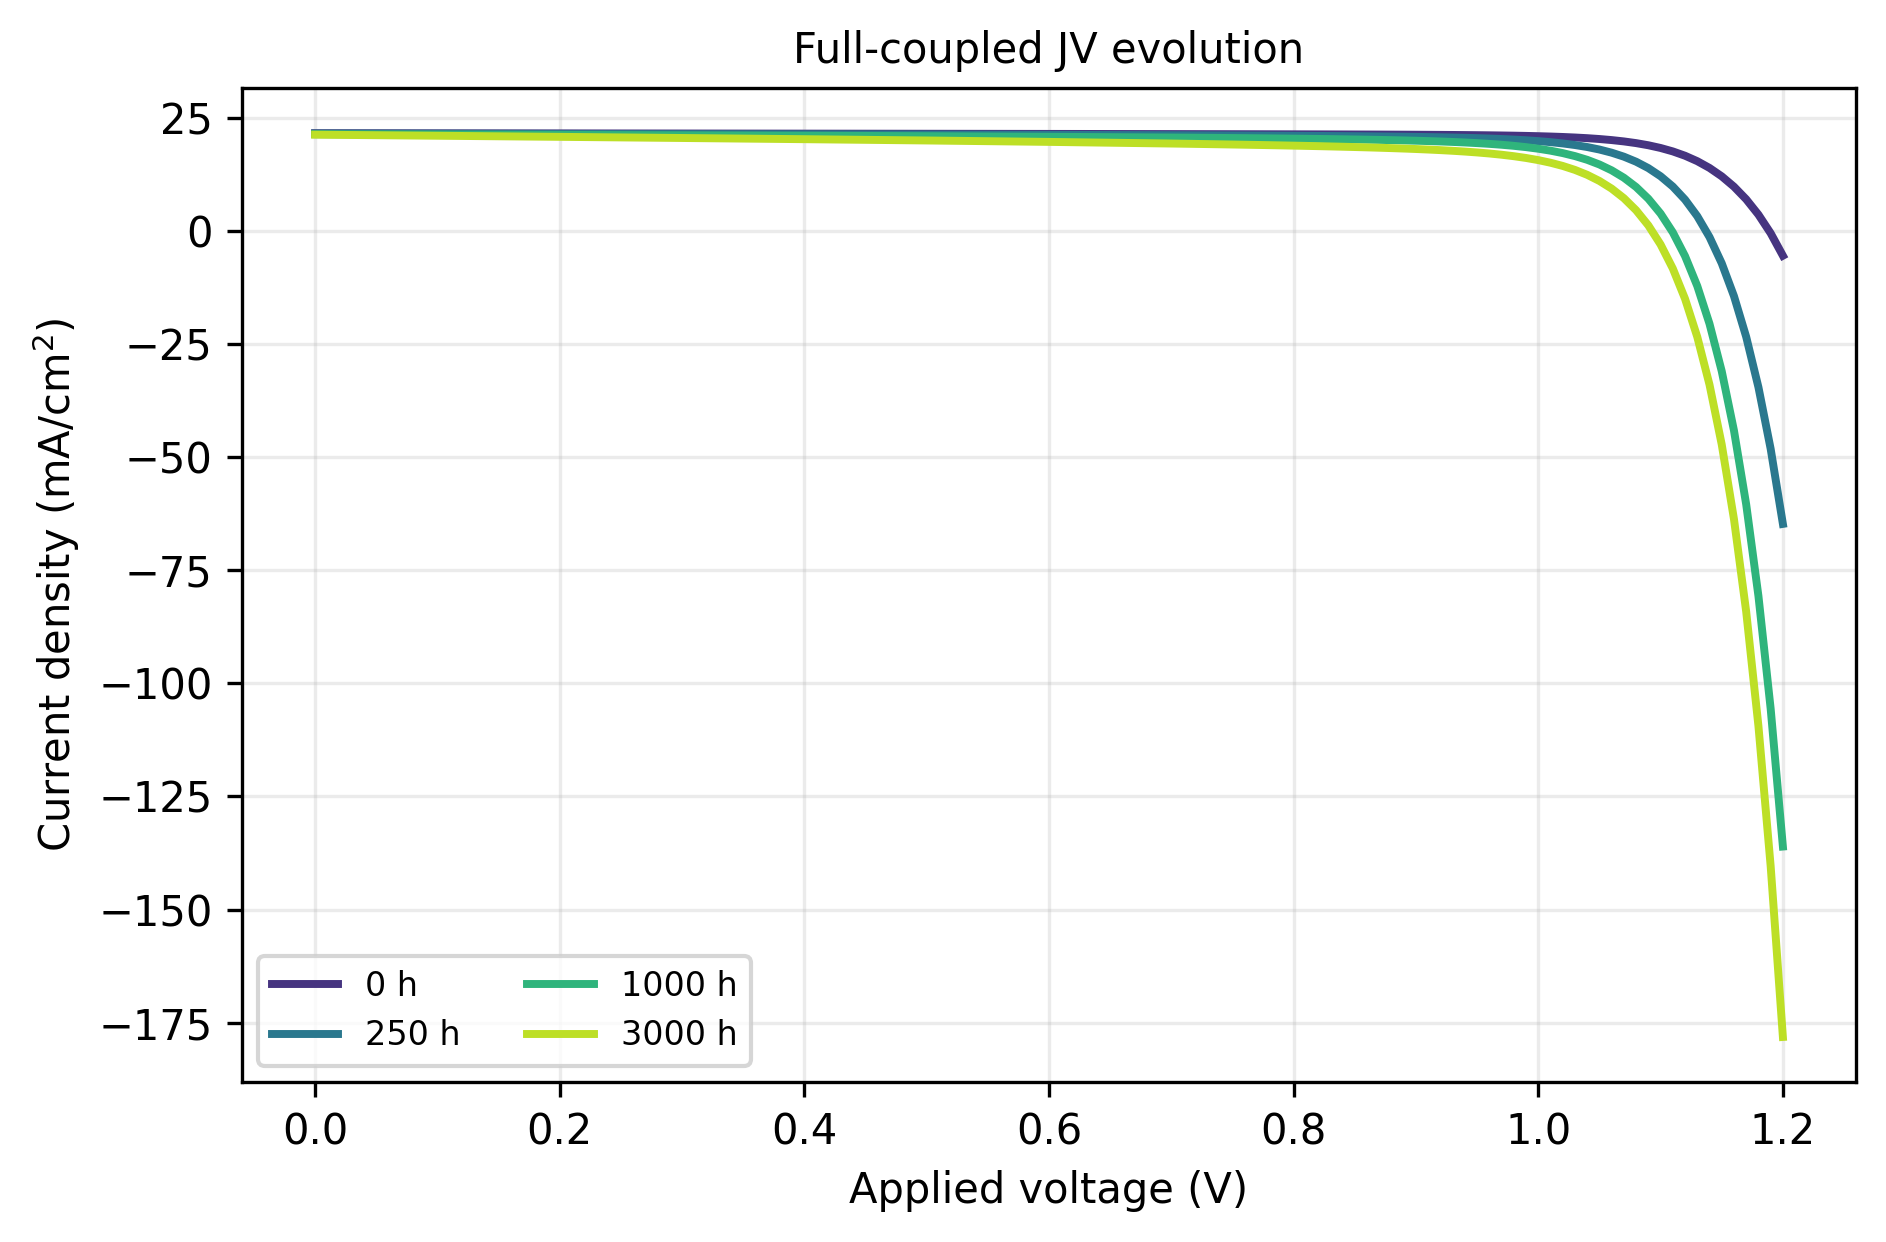
\includegraphics[width=0.82\textwidth]{outputs/figures/comsol_full_jv_evolution.png}
\caption{Full-coupled J--V evolution at selected aging times from the COMSOL sweep.}
\label{fig:comsol_full_jv}
\end{figure}

Figure~\ref{fig:comsol_full_jv} shows the full coupled J--V evolution. The
primary visible change is a downward and leftward shift near the knee region.
The variables that change are the effective recombination and resistance
parameters. Increased $N_t$ increases SRH recombination, reduced $R_{sh}$
increases leakage, and increased $R_s$ adds terminal voltage loss. The physical
mechanisms are trap growth, leakage-path formation, and contact or interface
degradation. The J--V signature is FF loss with accompanying PCE reduction.
The limitation is that similar knee collapse can result from several mechanism
combinations, so the curve shape must be interpreted with state trajectories
and independent calibration data.

\begin{figure}[H]
\centering
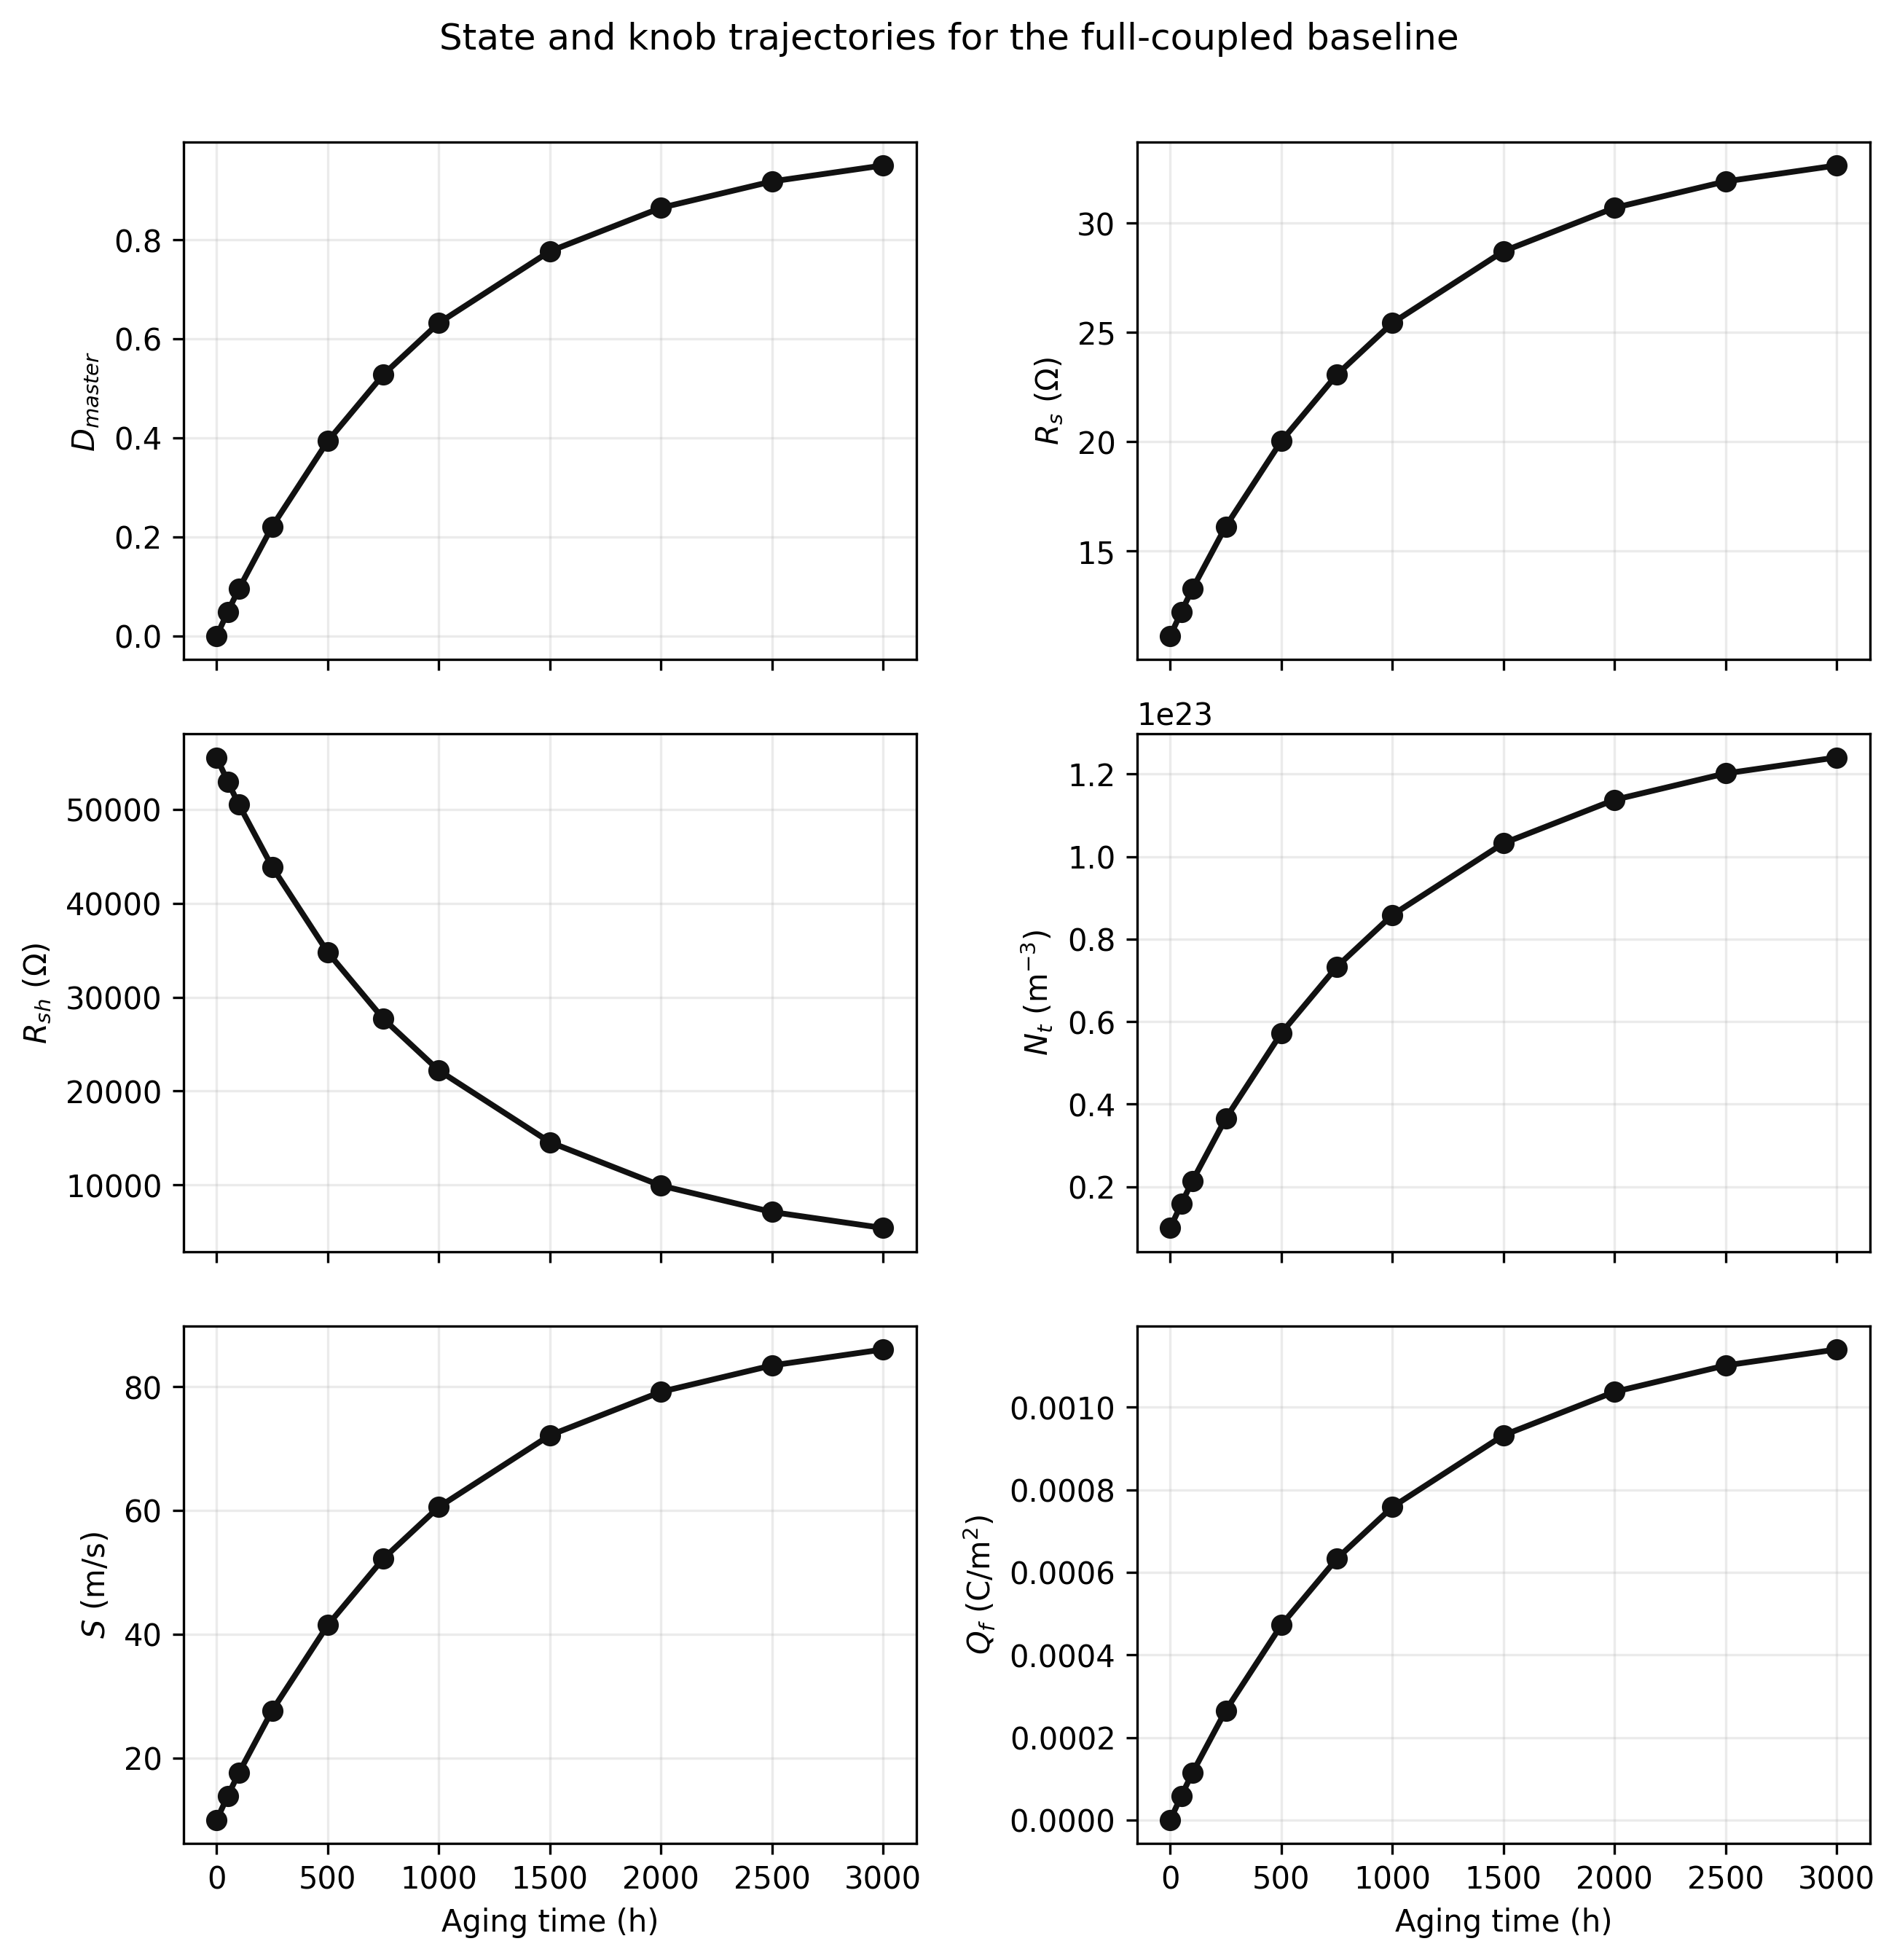
\includegraphics[width=0.92\textwidth]{outputs/figures/comsol_state_trajectories.png}
\caption{State and degradation-knob trajectories for the full coupled COMSOL baseline.}
\label{fig:comsol_state_trajectories}
\end{figure}

Figure~\ref{fig:comsol_state_trajectories} records the corresponding
degradation-parameter trajectories. The figure answers what the electrical
outputs respond to: bounded state variables map into COMSOL parameters over
aging time. This traceability is important because PCE loss alone does not
identify a mechanism. The limitation is that the state trajectories are
simulation inputs or coupled model states, not directly measured material
quantities unless additional experiments are used for calibration.

\section{Mechanism Sensitivity}

\begin{figure}[H]
\centering
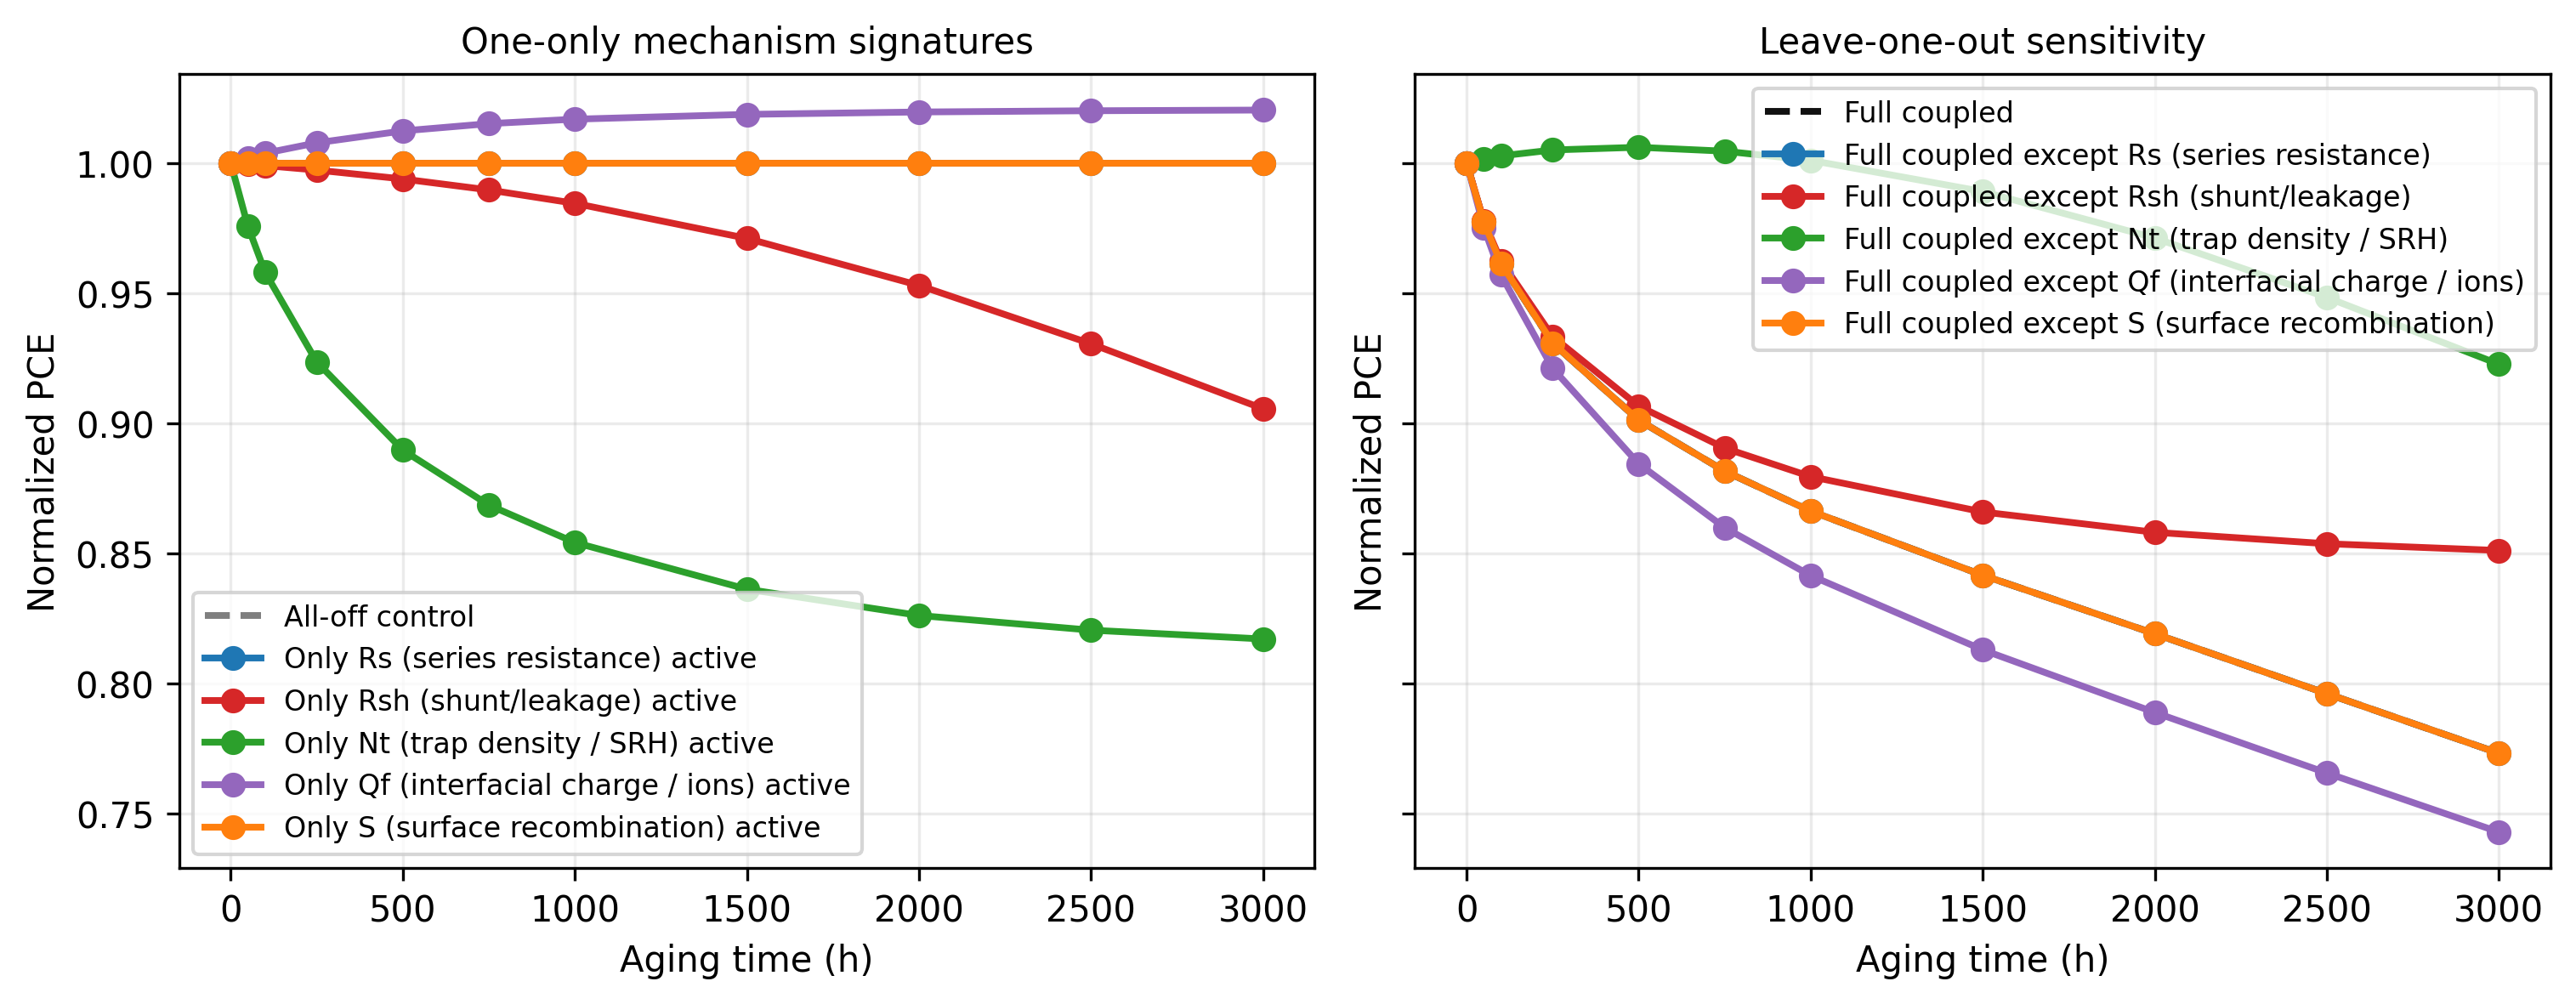
\includegraphics[width=\textwidth]{outputs/figures/comsol_mechanism_sensitivity.png}
\caption{One-only and leave-one-out mechanism sensitivity in the accelerated COMSOL scenario library.}
\label{fig:comsol_mechanism_sensitivity}
\end{figure}

Figure~\ref{fig:comsol_mechanism_sensitivity} compares one-only and
leave-one-out PCE responses. The one-only cases show that $N_t$ and $R_{sh}$
drive the strongest losses among the electrical observables, while $Q_f$ is
counteracting in this parameterization. The governing relations are the trap
density mapping in Eq.~\ref{eq:nt_linear}, the shunt mapping in
Eq.~\ref{eq:rsh_deg}, and the ionic or fixed-charge contribution to Poisson
electrostatics. The physical interpretation is that recombination and leakage
dominate the present terminal metrics, while charge redistribution can either
increase or decrease extracted power depending on how it changes band bending.
The mechanism ranking is qualitative because the amplitudes are selected for mechanism
separation rather than calibrated material degradation.

\begin{figure}[H]
\centering
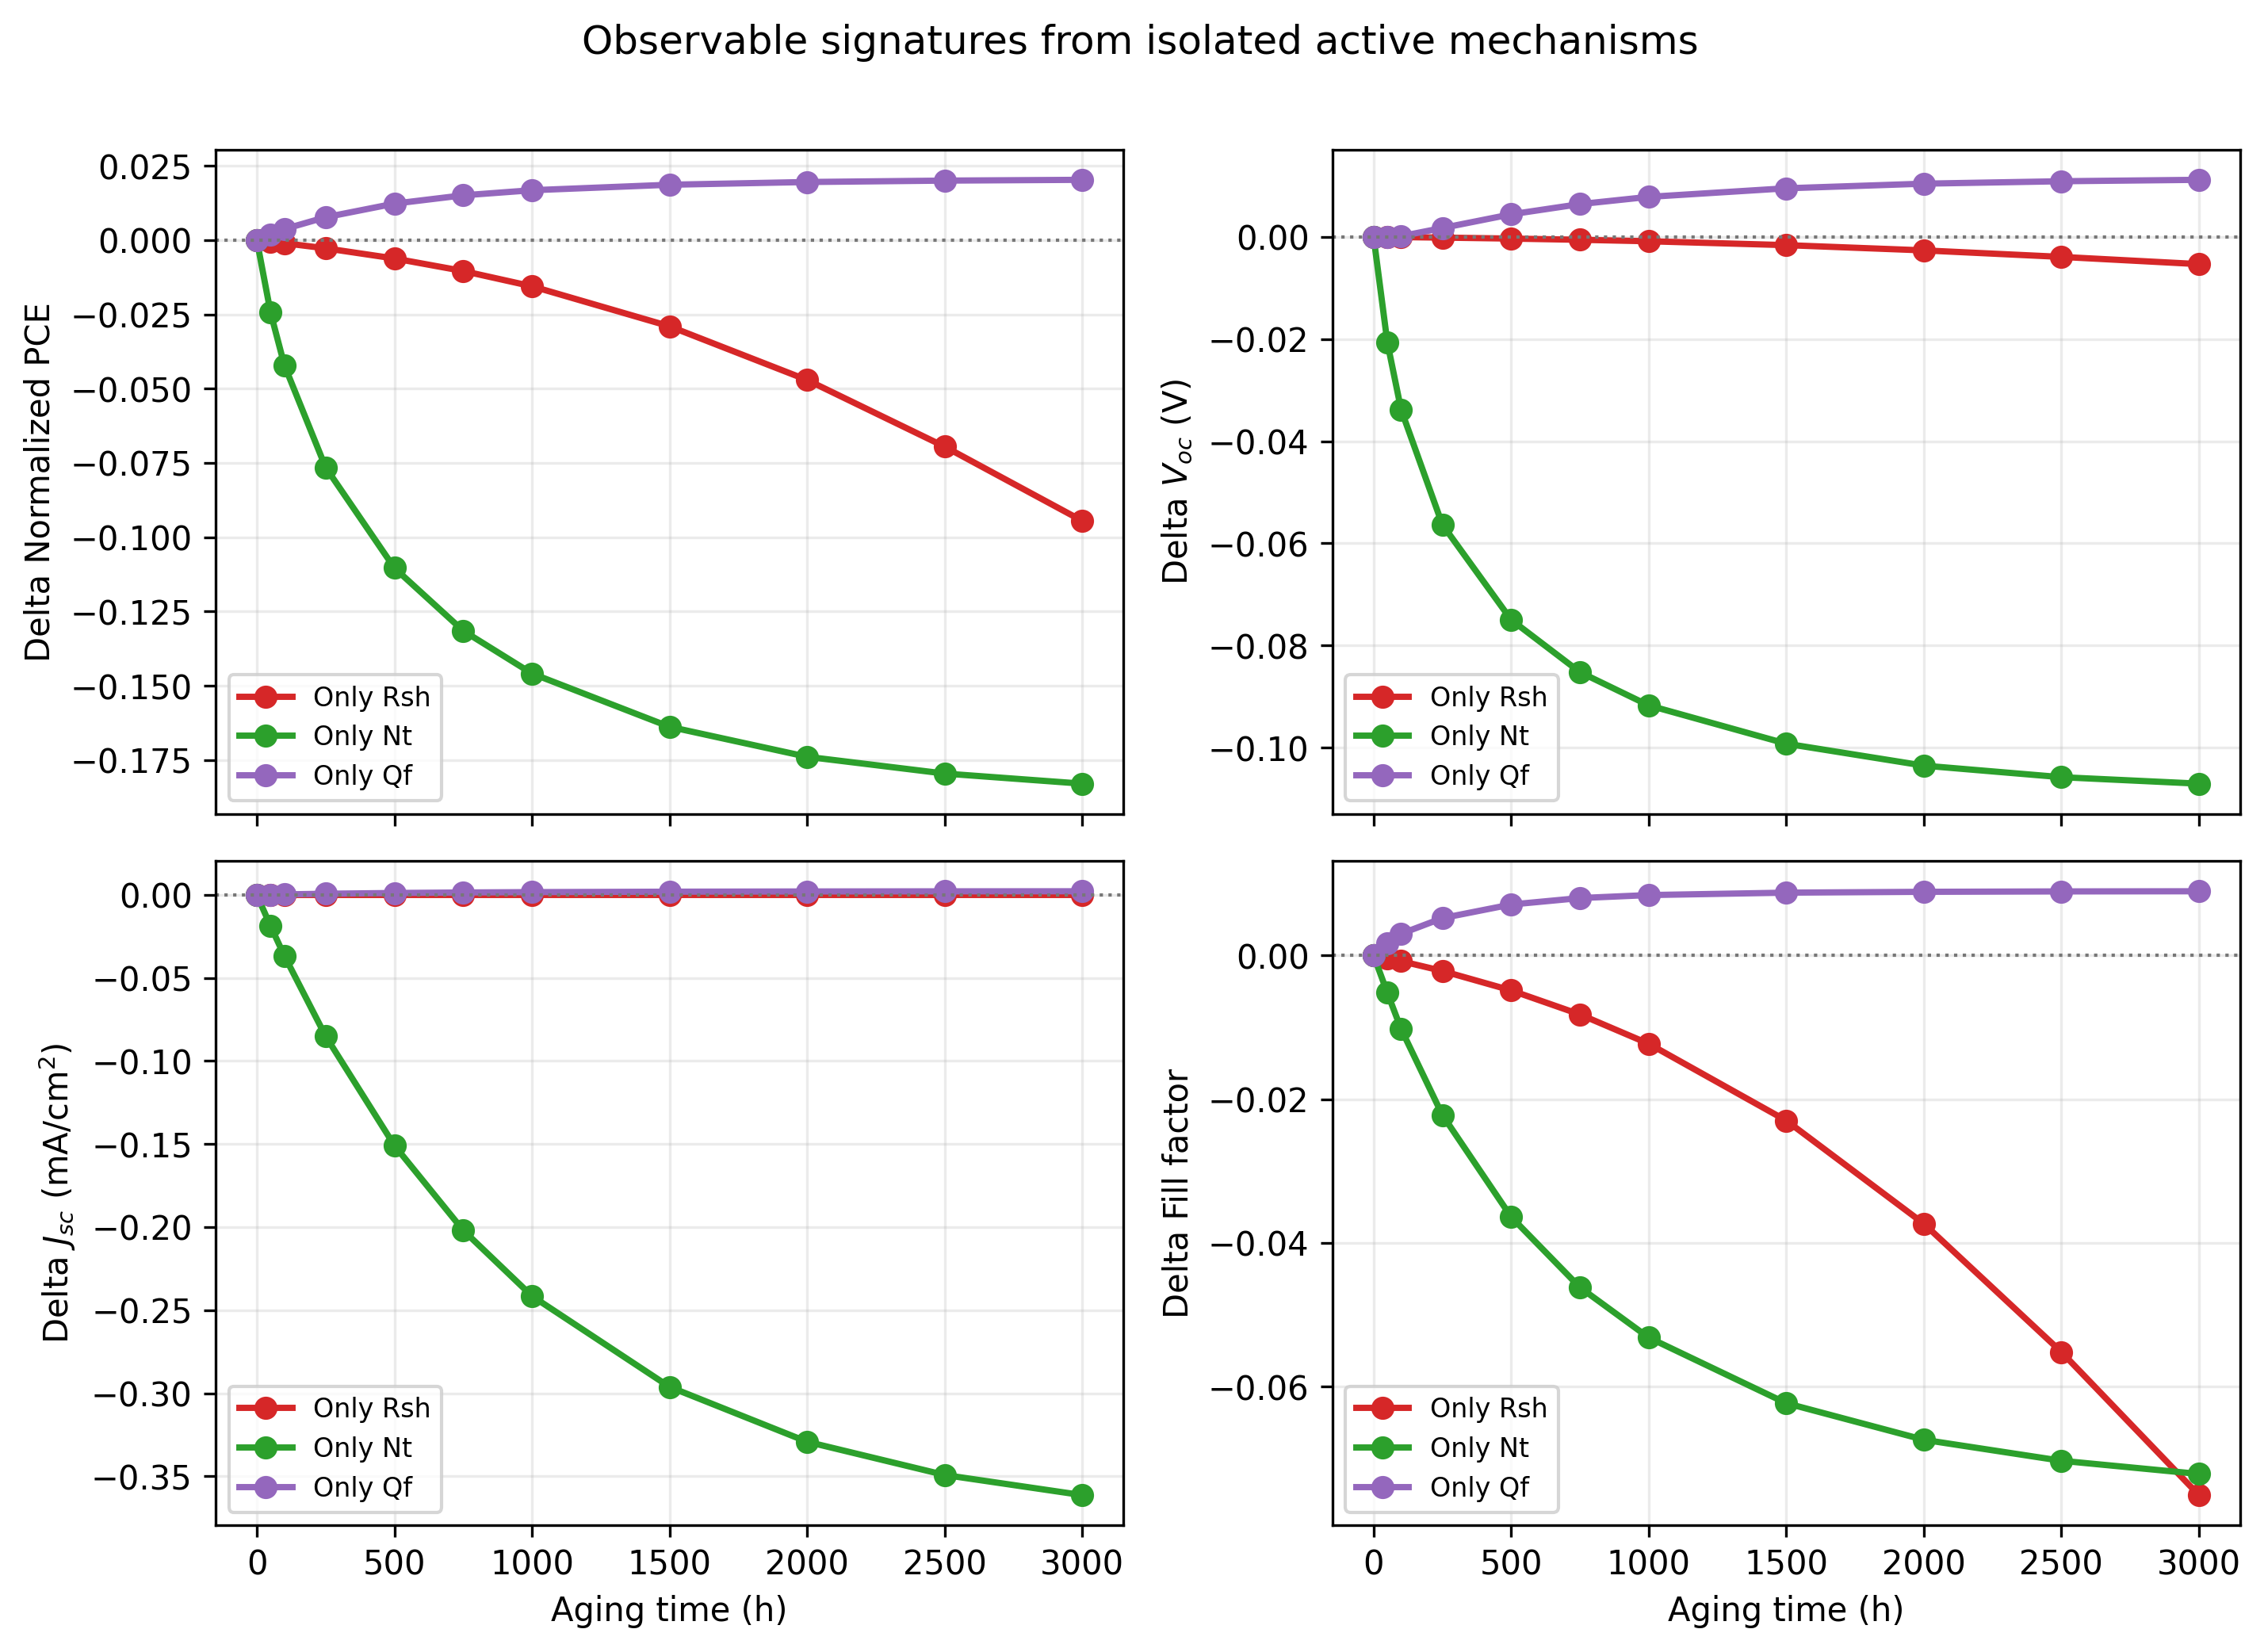
\includegraphics[width=\textwidth]{outputs/figures/comsol_metric_signatures.png}
\caption{Electrical observable signatures from the active one-only COMSOL mechanisms.}
\label{fig:comsol_metric_signatures}
\end{figure}

Figure~\ref{fig:comsol_metric_signatures} separates the J--V-derived metrics.
The $N_t$ case changes $V_{oc}$, $J_{sc}$, FF, and PCE because lifetime
reduction affects both voltage and collection. The $R_{sh}$ case is more
fill-factor dominated because leakage changes the low-bias slope. The $Q_f$
case has a smaller but nonzero counteracting signature because electrostatic
charge modifies internal fields. These signatures are useful for calibration
planning, but terminal metrics alone cannot uniquely identify all mechanisms.

\section{Electronic Parameter Sweep}

A separate COMSOL Global Evaluation export was used to sweep the baseline
electronic parameters $N_{t,0}$, $R_{s,0}$, and $R_{sh,0}$. Unlike the aging
library above, this sweep is not a time-evolving degradation trajectory. It is a
local electronic sensitivity study that checks whether the terminal J--V
signatures respond to the expected physical parameter directions. The export
contains 819 parameter combinations. The post-processing script extracts the
active voltage-ramp segment from each transient scan and computes PCE,
$V_{oc}$, $J_{sc}$, FF, $V_{\mathrm{mpp}}$, and $J_{\mathrm{mpp}}$.

\begin{table}[H]
\centering
\caption{Summary of the one-parameter-at-a-time COMSOL electronic sweep. The
held parameters are fixed at the model reference values:
$N_{t,0}=10^{16}~\mathrm{cm^{-3}}$, $R_{s,0}=1~\Omega\mathrm{cm^2}$, and
$R_{sh,0}=10^{5}~\Omega\mathrm{cm^2}$. The PCE ranges report the extrema from
that one-parameter-at-a-time slice, not the best point from the full
all-combination grid.}
\label{tab:parameter_sweep_summary}
\begin{tabular}{@{}p{0.13\textwidth}p{0.25\textwidth}p{0.17\textwidth}p{0.34\textwidth}@{}}
\toprule
Sweep & Parameter range & PCE range & Main response and interpretation \\
\midrule
$N_{t,0}$ &
$10^{14}$--$10^{20}~\mathrm{cm^{-3}}$ &
19.01--17.08\% &
$V_{oc}$ and $J_{sc}$ decrease, consistent with stronger bulk recombination. \\
$R_{s,0}$ &
0.1--$10~\Omega\mathrm{cm^2}$ &
19.42--15.90\% &
FF decreases from 0.812 to 0.665, consistent with series loss. \\
$R_{sh,0}$ &
$10^{3}$--$10^{6}~\Omega\mathrm{cm^2}$ &
18.06--19.01\% &
FF improves from 0.757 to 0.795 as leakage is suppressed. \\
\bottomrule
\end{tabular}
\end{table}

\begin{figure}[H]
\centering
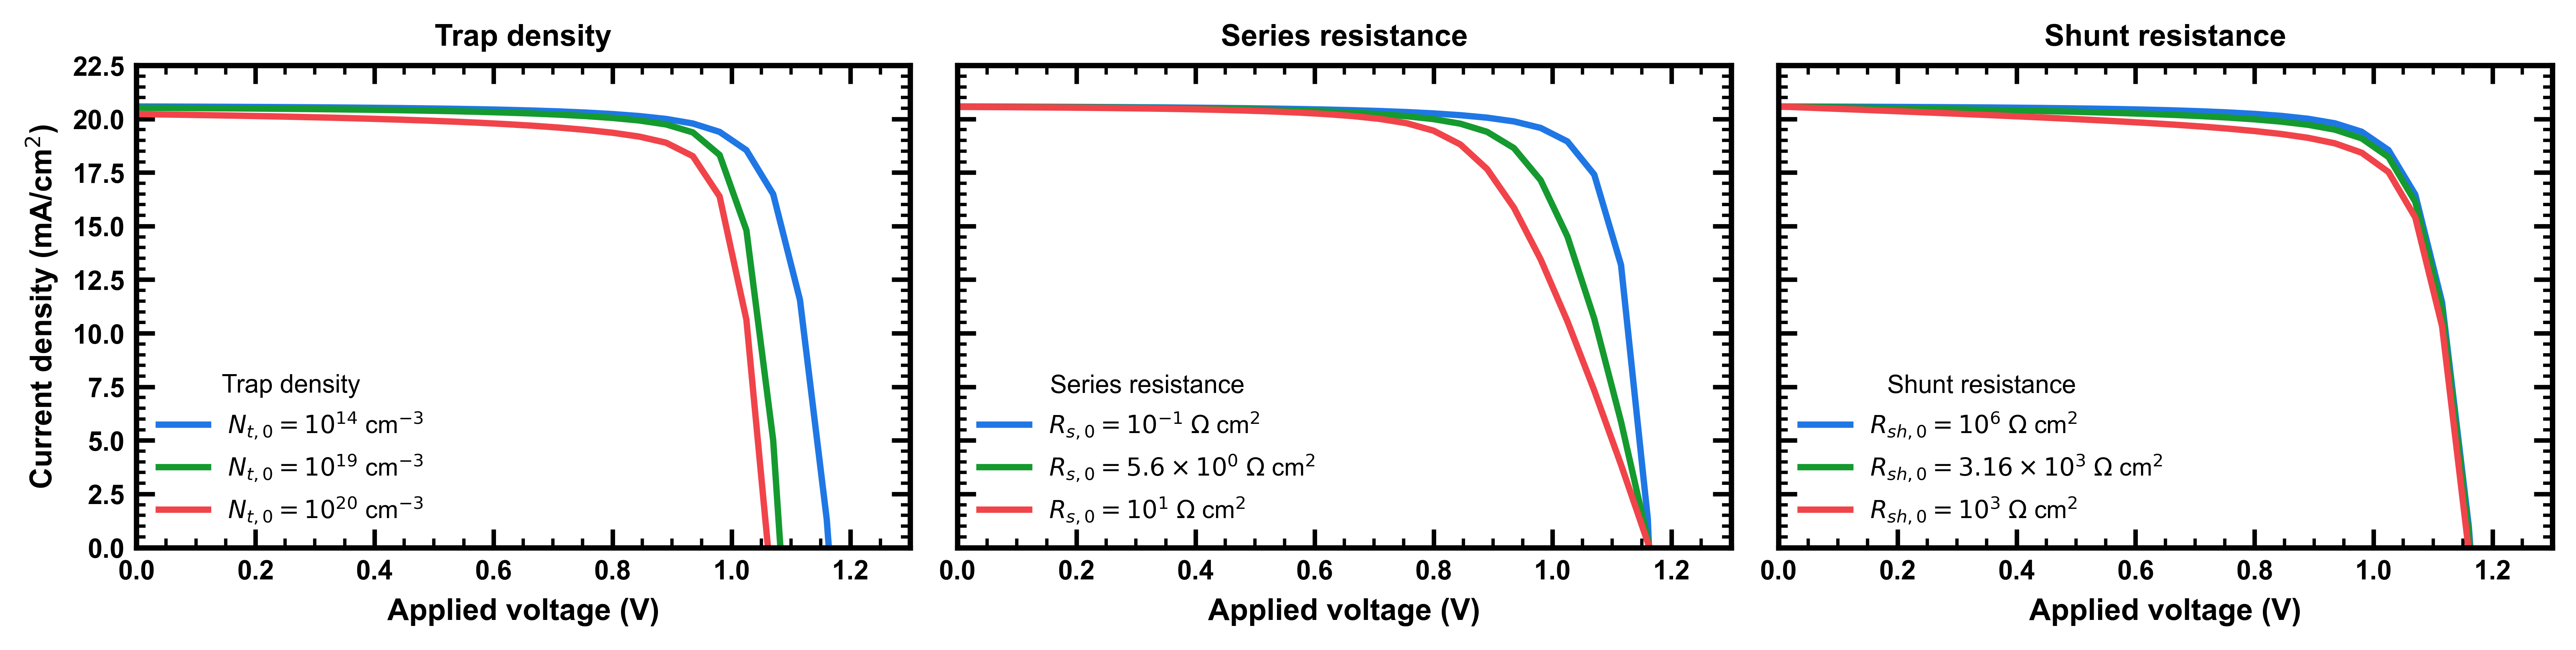
\includegraphics[width=\textwidth]{outputs/figures/comsol_parameter_sweep/comsol_parameter_sweep_jv_examples.png}
\caption{Representative J--V curves from the COMSOL electronic parameter
sweep. Each panel varies one parameter while holding the other two at the
baseline values used in Table~\ref{tab:parameter_sweep_summary}.}
\label{fig:comsol_parameter_sweep_jv}
\end{figure}

Figure~\ref{fig:comsol_parameter_sweep_jv} shows the expected qualitative
terminal signatures. Larger $R_{s,0}$ reduces the high-power knee and lowers
fill factor. Lower $R_{sh,0}$ increases leakage and reduces the low-bias
quality of the curve. Larger $N_{t,0}$ reduces the achievable voltage and
current through recombination. These trends support the interpretation of the
mechanism-isolation library, but they still do not uniquely invert a measured
J--V curve to one material parameter.

\begin{figure}[H]
\centering
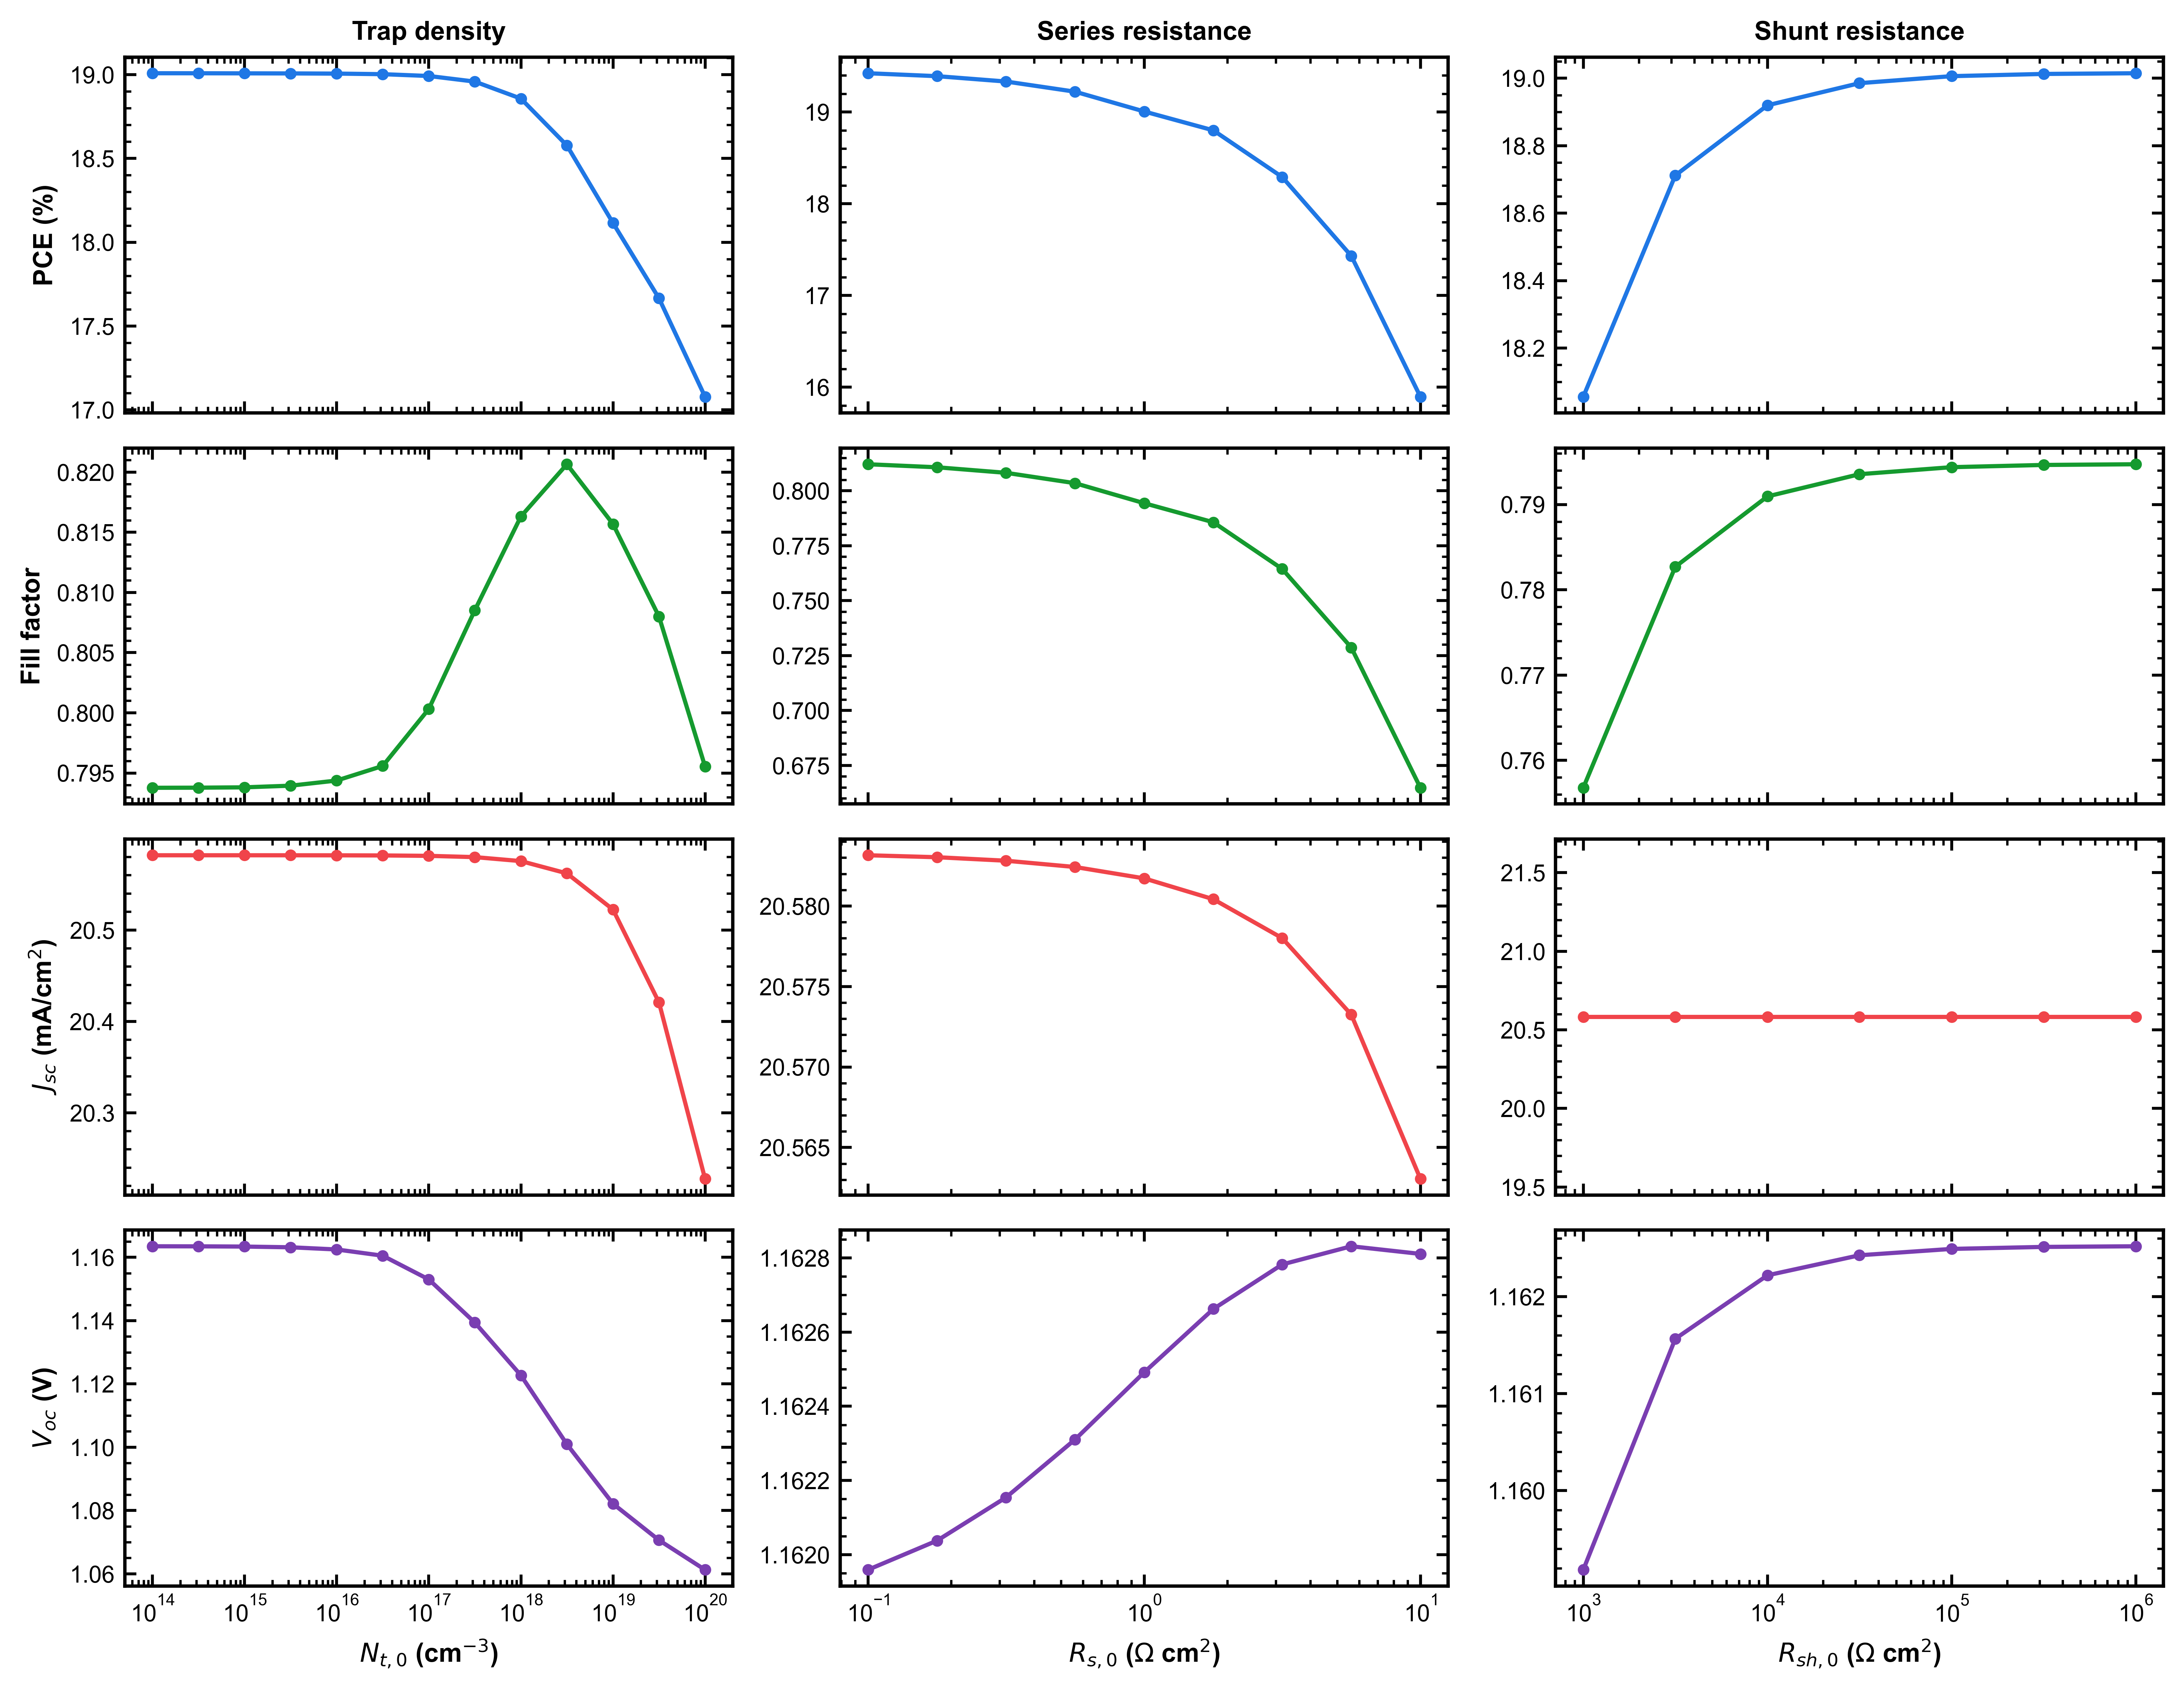
\includegraphics[width=\textwidth]{outputs/figures/comsol_parameter_sweep/comsol_parameter_sweep_metrics_all.png}
\caption{Extracted PCE, fill factor, $J_{sc}$, and $V_{oc}$ for the
one-parameter-at-a-time COMSOL electronic sweep. The full processed table
contains 819 all-combination rows, of which 795 remain above 15\% PCE in this
export.}
\label{fig:comsol_parameter_sweep_metrics}
\end{figure}

Figure~\ref{fig:comsol_parameter_sweep_metrics} converts the J--V curves into
scalar photovoltaic metrics. In this export, the best-performing full-factorial
grid point
has PCE $=19.44\%$, $V_{oc}=1.163$ V, $J_{sc}=20.58~\mathrm{mA/cm^2}$, and
FF $=0.812$. The all-combination sweep spans 13.42--19.44\% PCE. This range is
useful for identifying plausible calibration directions and for defining
future surrogate-model input ranges. It should not be interpreted as an
optimized device design because optical, transport-layer, ion, and degradation
parameters remain fixed.

\section{Architecture-Stress Aging Grid}

The later COMSOL exports extend the thesis data set from static electronic
parameter sweeps to architecture-scoped aging outputs. The current canonical
architecture-stress J--V export,
\path{data/raw/comsol/arch_baseline_pin/Aging/Stress_matrix_jv_003.csv},
stores a full light-temperature diagnostic J--V sweep as a concatenated
two-column table. The post-processing script splits this file into 360 J--V
curves using the COMSOL parameter ordering shown in the export: ten aging
checkpoints and 36 light-temperature scenarios. The scenario grid matches the
profile-grid stress matrix, with aging temperatures of 300--400 K and aging
displayed light levels of 0--1.00 sun, where the plotted 0-sun case is the
COMSOL 0.01-sun numerical floor. This export gives a direct electrical map of
the light-plus-temperature degradation surface. The voltage range ends at
1.25 V, so some low-temperature and early-aging curves do not cross zero
current. PCE and $J_{sc}$ are therefore retained for all curves, while
$V_{oc}$ and FF are reported only for curves with a resolved zero-current
crossing. Earlier files in the same folder,
\path{Stress_matrix_jv_001.csv} and \path{Stress_matrix_jv_002.csv}, are
superseded development exports and are retained only for audit history.

\begin{figure}[H]
\centering
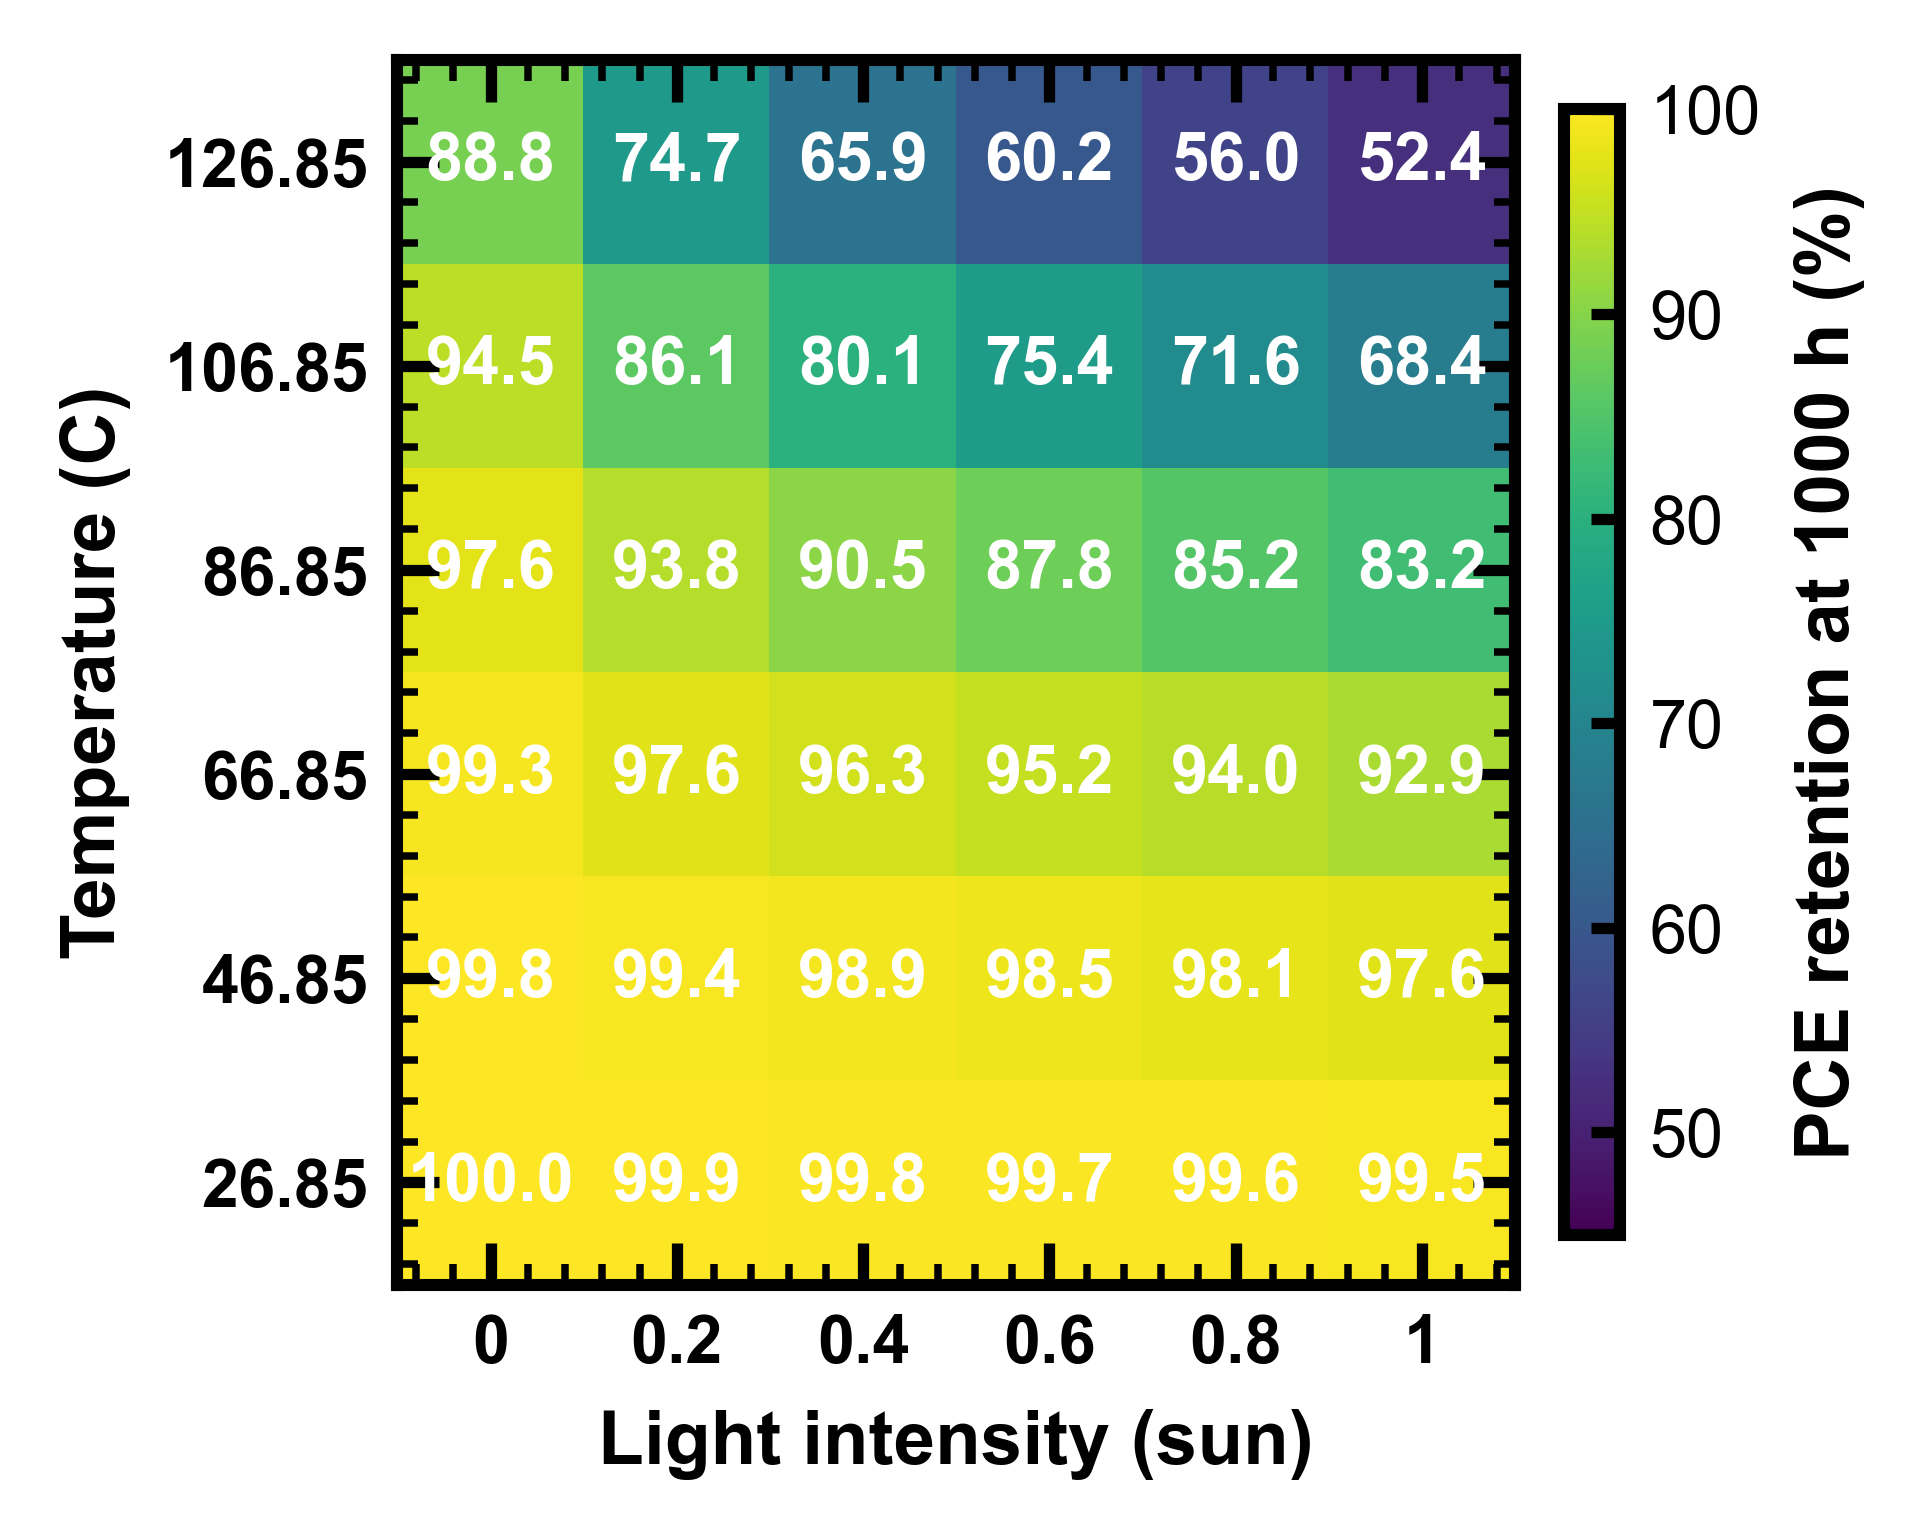
\includegraphics[width=0.72\textwidth]{outputs/figures/comsol_architecture_stress_grid/baseline_pin_stress_matrix_jv_003_pce_retention_heatmap.png}
\caption{Final PCE retention from the 360-curve light-temperature J--V export. The result shows coupled light and heat acceleration: 1000 h retention remains near 100\% at 300 K and low light, but decreases to 52.4\% at 400 K and one sun.}
\label{fig:baseline_pin_temperature_pce_retention_flat}
\end{figure}

\begin{figure}[H]
\centering
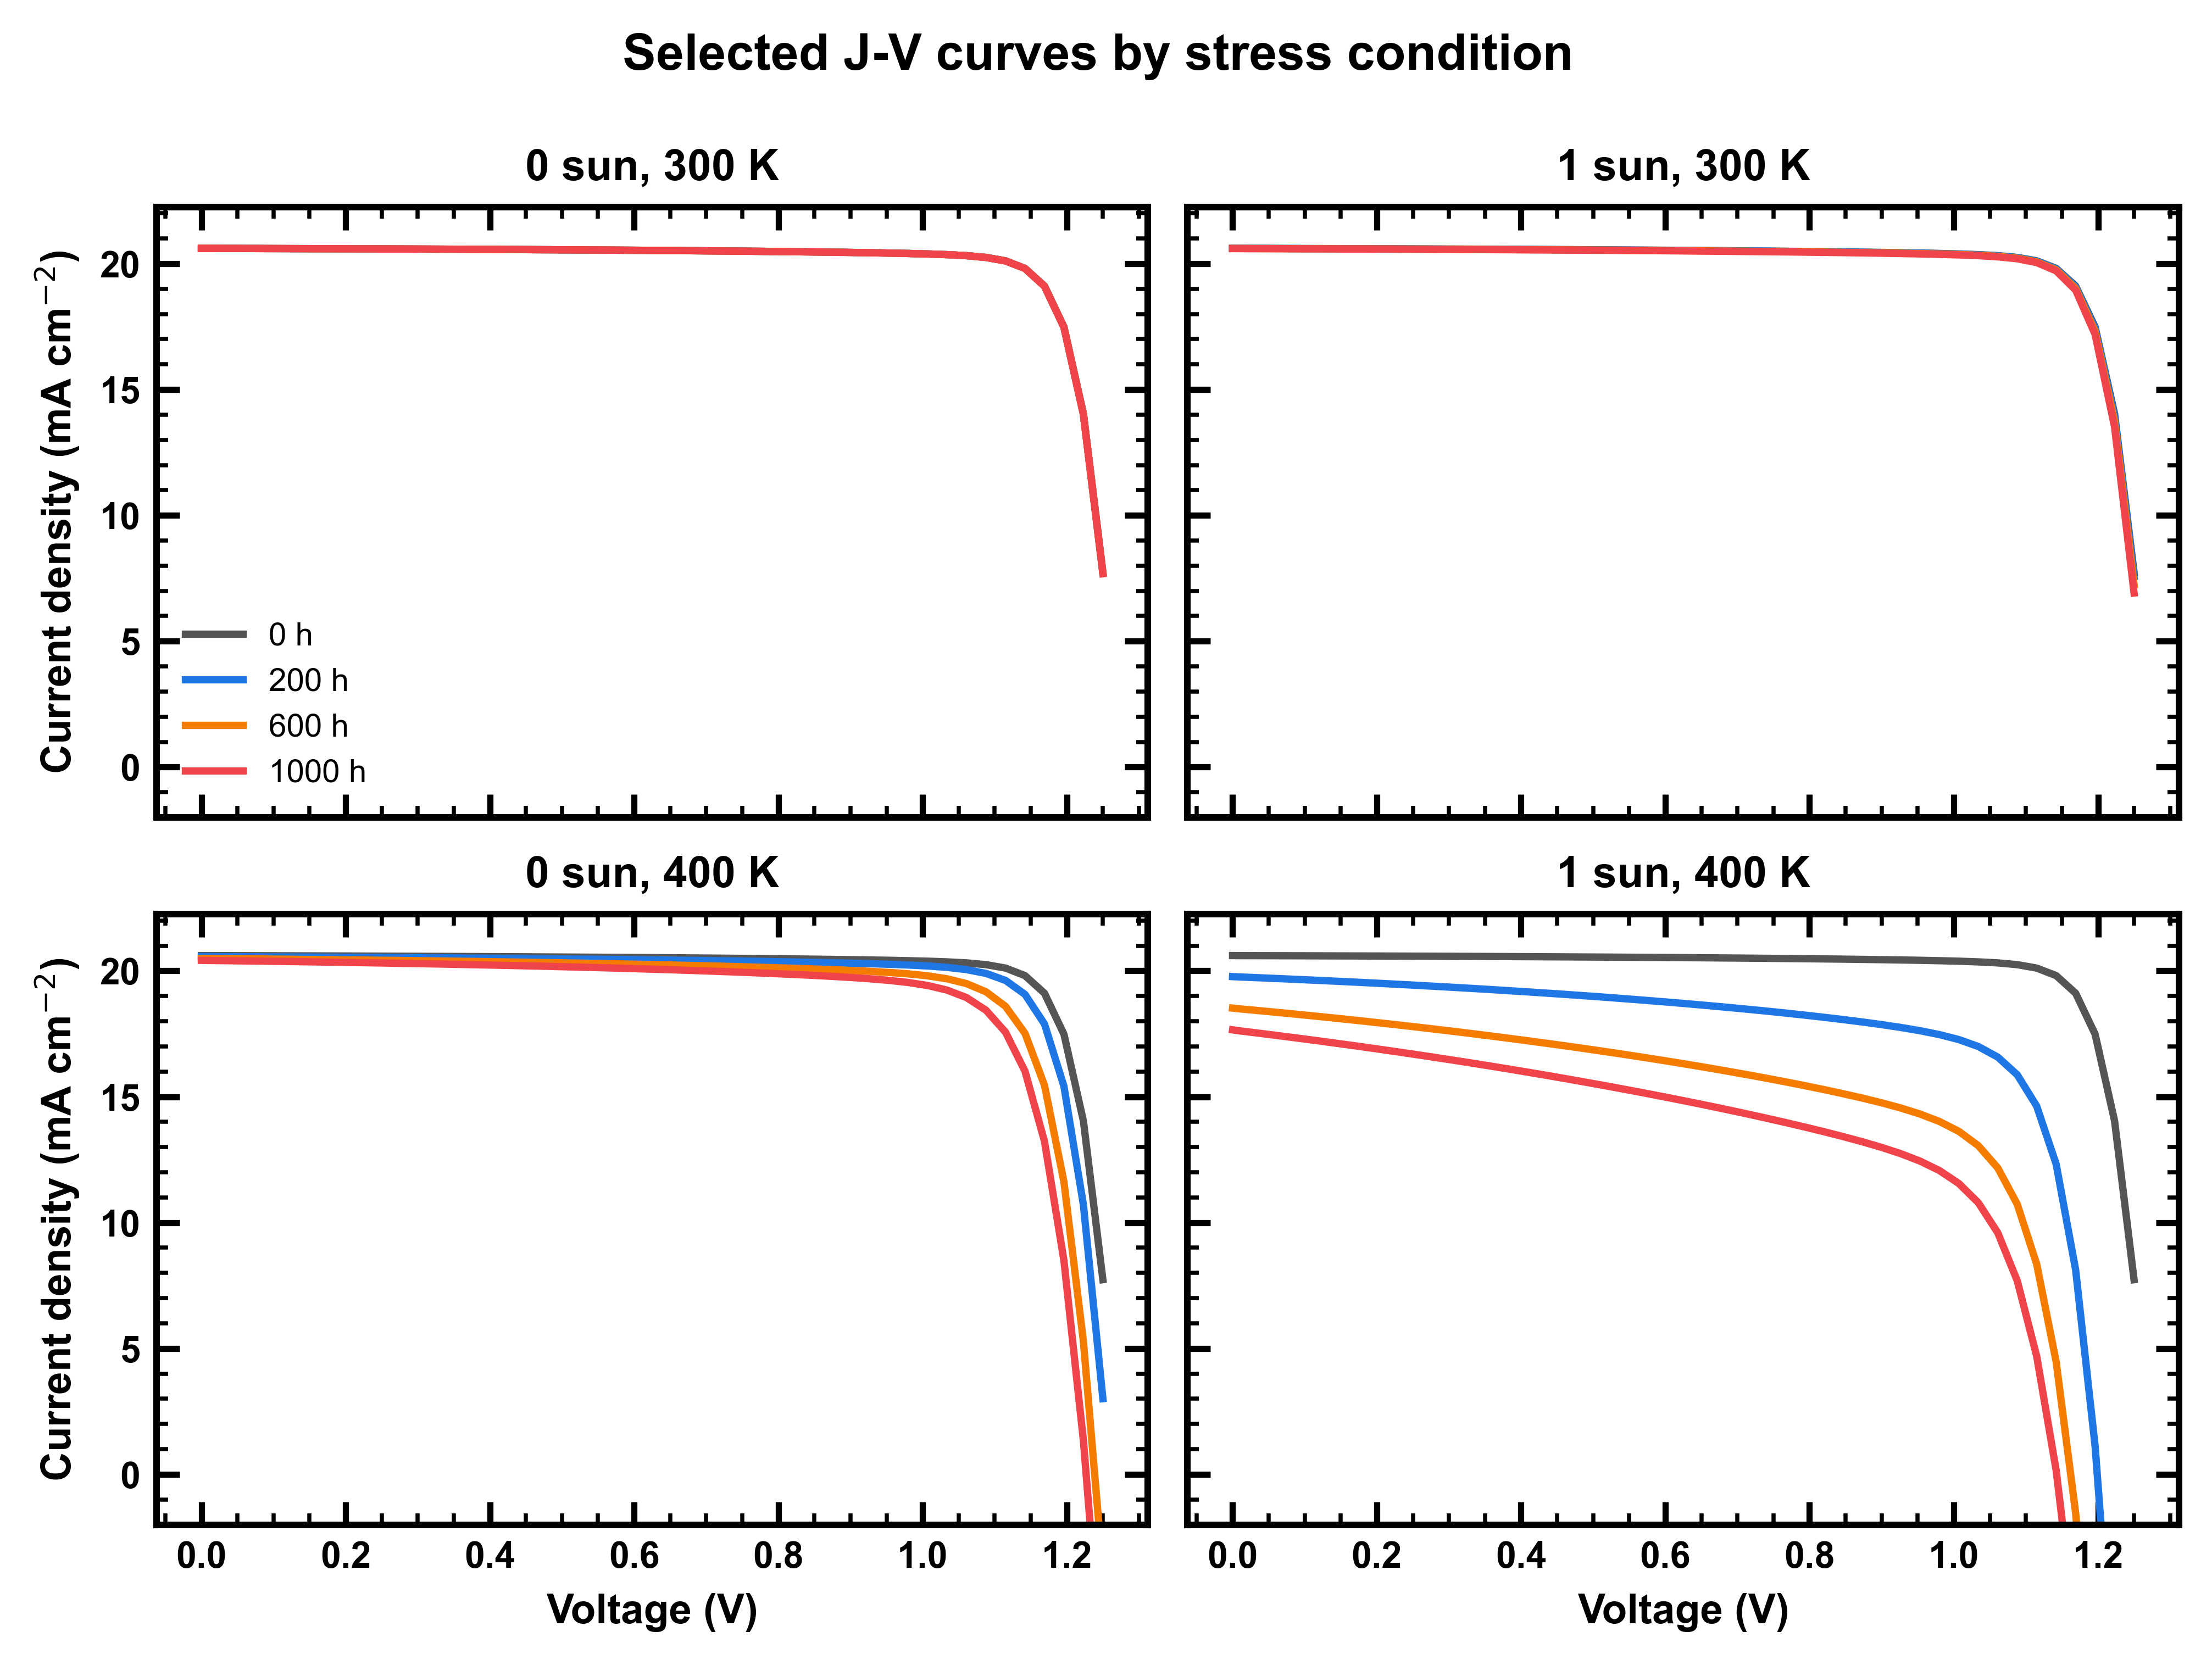
\includegraphics[width=\textwidth]{outputs/figures/comsol_architecture_stress_grid/baseline_pin_stress_matrix_jv_003_jv_selected.png}
\caption{Representative corner J--V curves from the flat light-temperature export. The high-temperature, one-sun case shows stronger $J_{sc}$ loss and knee rounding with aging, while the low-temperature cases remain close to the initial curve over the same equivalent aging window.}
\label{fig:baseline_pin_temperature_jv_flat}
\end{figure}

\section{Light-Temperature Internal-State Profile Grid}

A separate 6 $\times$ 6 profile-grid export was organized for the baseline
p-i-n architecture. It covers aging temperatures of 300, 320, 340, 360, 380,
and 400 K and displayed aging light levels of 0, 0.20, 0.40, 0.60, 0.80, and
1.00 sun. The 0-sun label corresponds to the COMSOL 0.01-sun numerical floor.
Each file contains spatial profiles at ten aging checkpoints for
$u_{\mathrm{ion}}$, $D_{\mathrm{trap}}$, $D_{Rs}$, $D_{Rsh}$,
$N_{t,\mathrm{eff}}$, SRH recombination, and electric field. This grid is the
first data product in the thesis that directly connects terminal J--V trends
to internal state variables across a light-temperature stress matrix.

\begin{figure}[H]
\centering
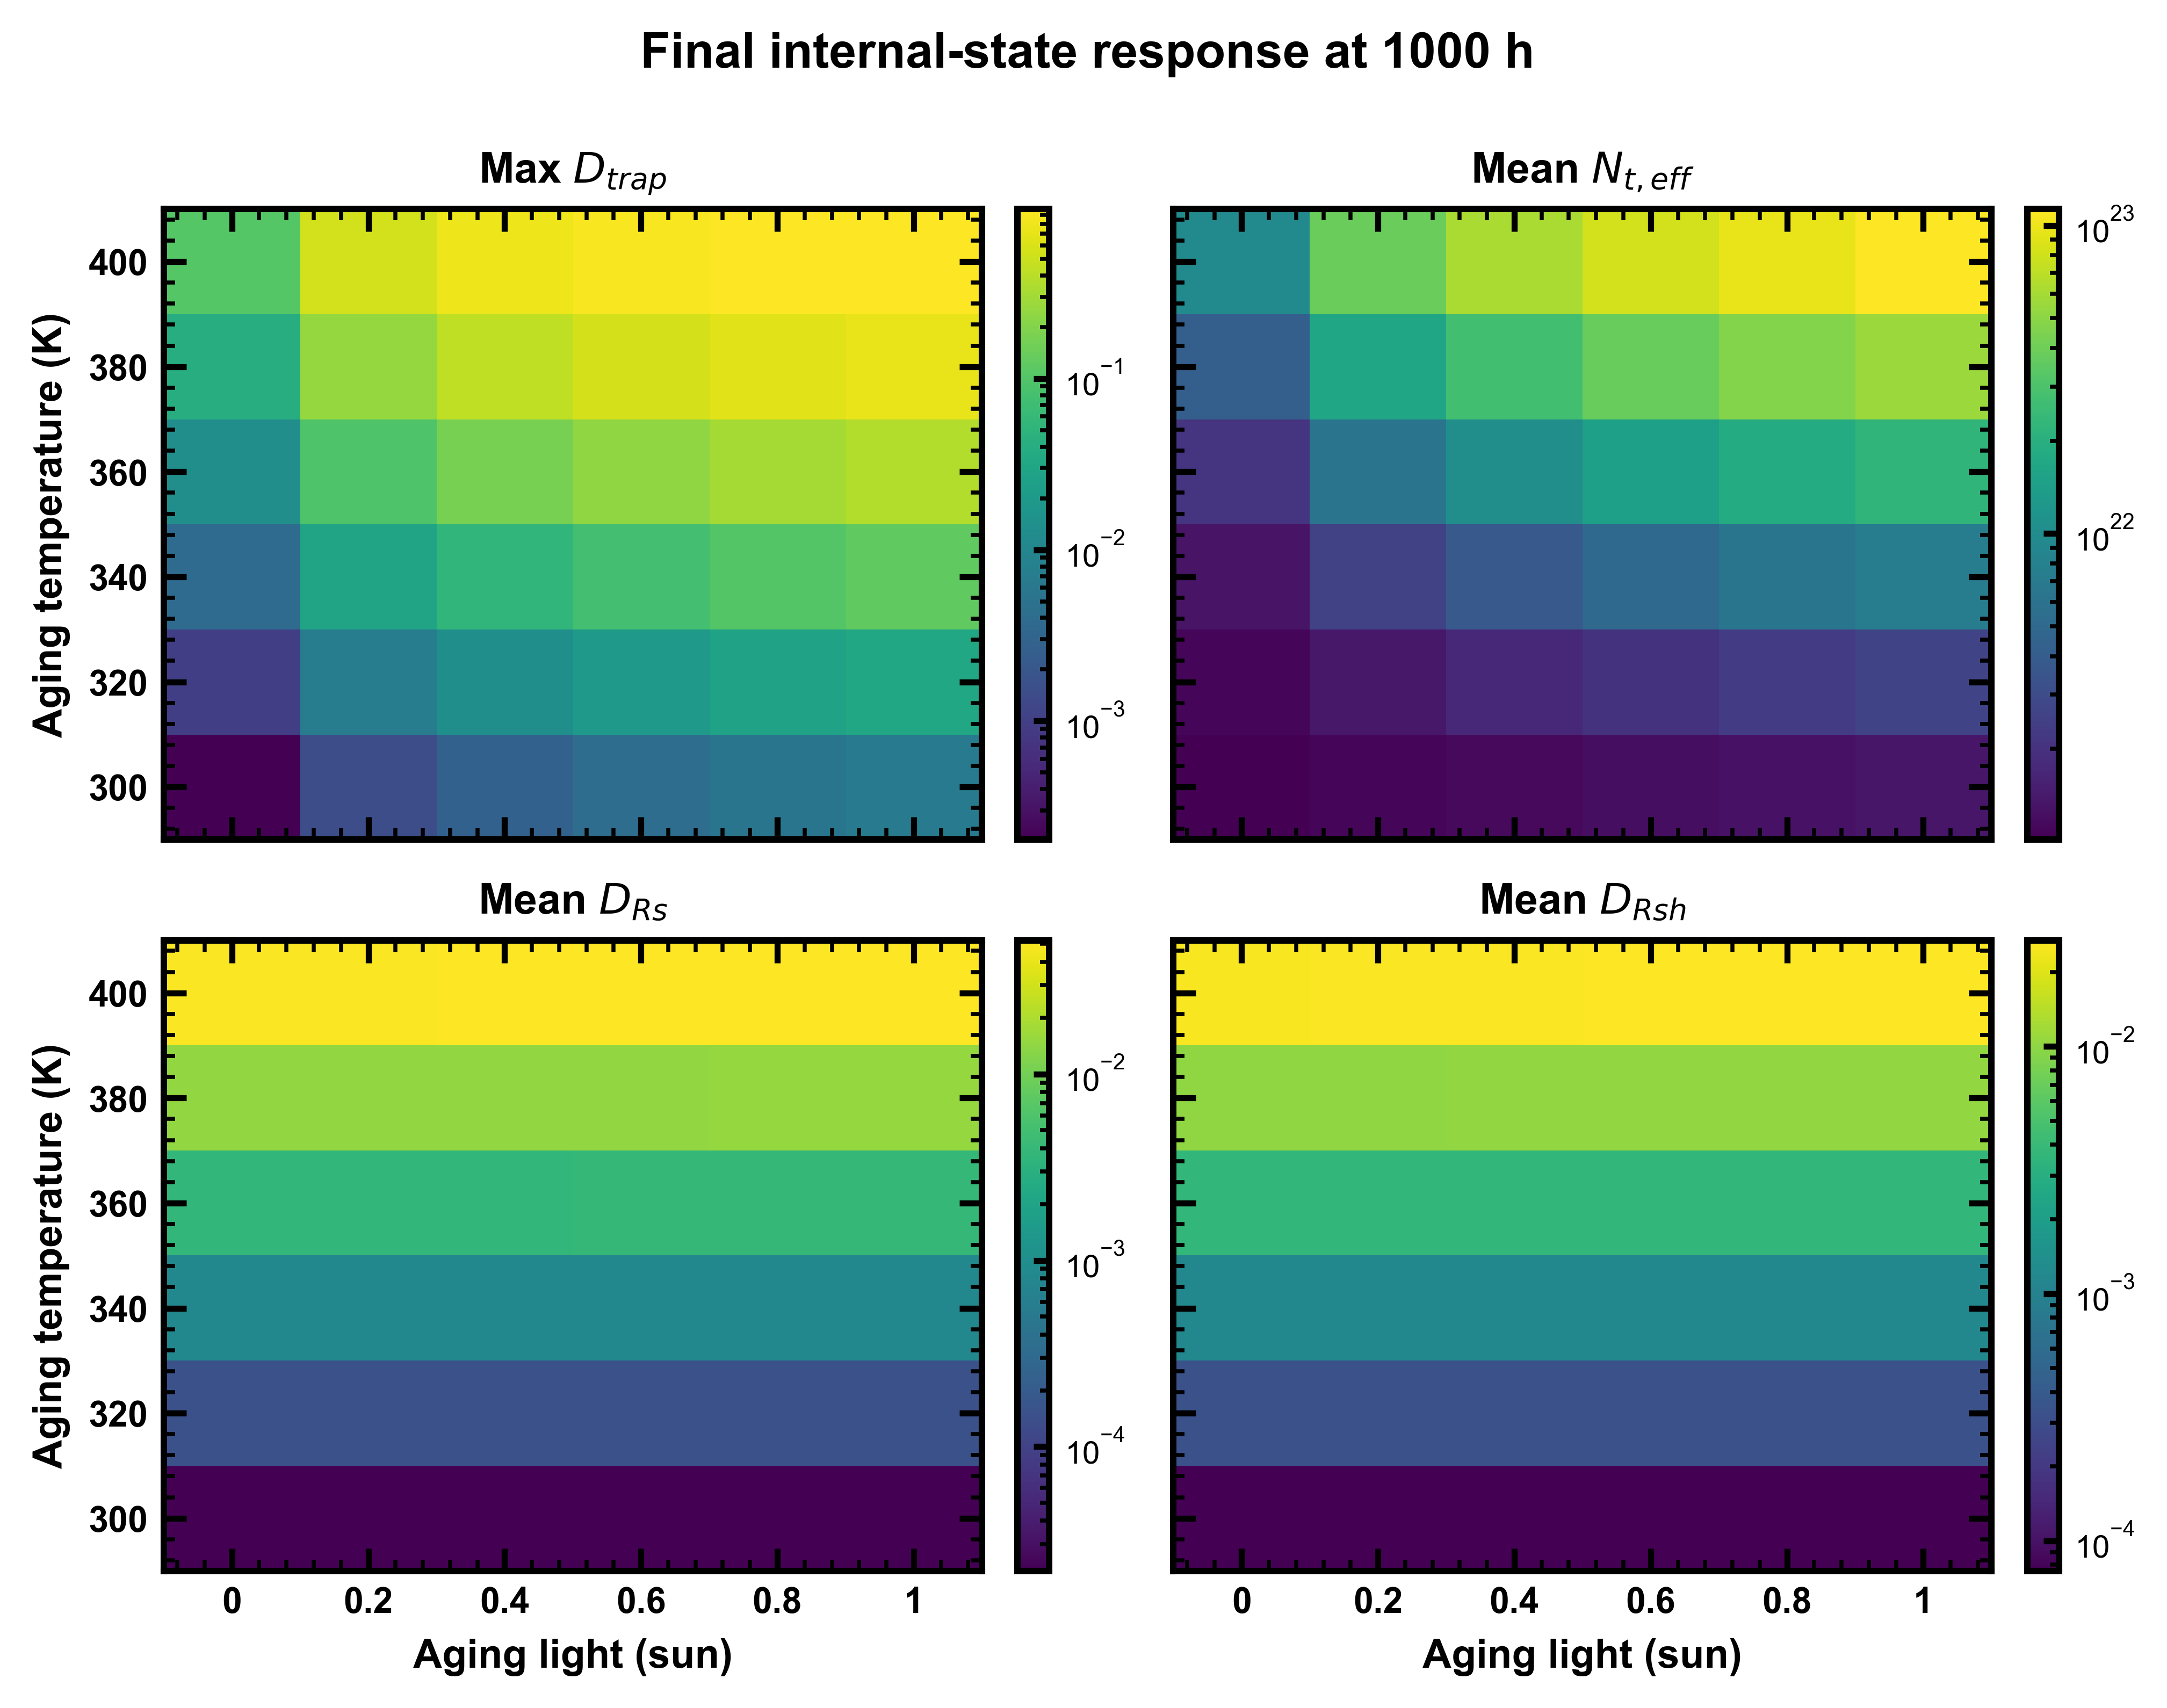
\includegraphics[width=\textwidth]{outputs/figures/comsol_architecture_stress_grid/profile_grid_final_state_summary.png}
\caption{Final 1000 h internal-state response from the baseline p-i-n 6 $\times$ 6 light-temperature profile grid. Trap damage and effective trap density increase with both light and temperature, while the resistance-damage states are dominated mainly by the temperature axis in this export.}
\label{fig:profile_grid_final_state_summary}
\end{figure}

\begin{table}[H]
\centering
\caption{Final 1000 h extrema from the baseline p-i-n light-temperature profile grid. The table reports where each state summary is smallest and largest across the 6 $\times$ 6 stress grid.}
\label{tab:profile_grid_extrema}
\begin{tabular}{@{}lrrrrrr@{}}
\toprule
State summary & Min & $T$ (K) & Light & Max & $T$ (K) & Light \\
\midrule
max $D_{\mathrm{trap}}$ & 0.000204 & 300 & 0 & 0.975 & 400 & 1 \\
max $u_{\mathrm{ion}}$ & 59 & 400 & 1 & 77.2 & 300 & 0 \\
mean $D_{Rs}$ & 2.16e-05 & 300 & 1 & 0.0522 & 400 & 1 \\
mean $D_{Rsh}$ & 7.57e-05 & 300 & 1 & 0.0268 & 400 & 1 \\
mean $N_{t,\mathrm{eff}}$ & 1.02e+21 & 300 & 0 & 1.13e+23 & 400 & 1 \\
\bottomrule
\end{tabular}
\end{table}


Figure~\ref{fig:profile_grid_final_state_summary} and
Table~\ref{tab:profile_grid_extrema} show the expected stress ordering for the
irreversible trap and resistance-damage states. The smallest final trap
response occurs at the lowest light and temperature, while the largest final
trap and effective trap-density responses occur at 400 K and one sun. The
resistance-damage states increase by orders of magnitude with temperature but
are comparatively weakly dependent on light in this parameterization. The
maximum mobile-ion accumulation should be interpreted differently: it is a
redistribution diagnostic controlled by electric field, thermal voltage, and
preconditioning state, not a monotonic irreversible damage variable. This
distinction is useful for future inverse modeling: a terminal J--V curve alone
may not separate trap growth from resistance evolution, but a COMSOL-generated
state grid can define the physically plausible state manifold for surrogate
training.

\section{Lite COMSOL-Trained Surrogate Baseline}

The validated light-temperature J--V export and profile-grid summaries also
define the first traceable machine-learning data product in the thesis. The
purpose of this section is limited: it tests whether the current COMSOL export
contract can support a forward surrogate with scenario-held-out validation. It
does not claim a final experimentally calibrated digital twin, and it does not
train an inverse model from measured data. The reproducible entry point is
\path{scripts/train_lite_surrogates.py}, which reads the processed COMSOL
tables, encodes the stored 0.01-sun numerical floor as the displayed 0-sun
condition, trains lightweight random-forest baselines, and writes model files,
validation predictions, figures, tables, and metadata under
\path{models/surrogate_lite/},
\path{outputs/figures/surrogate_lite/}, and
\path{outputs/tables/surrogate_lite/}.

\begin{figure}[H]
\centering
\begin{minipage}{0.49\textwidth}
\centering
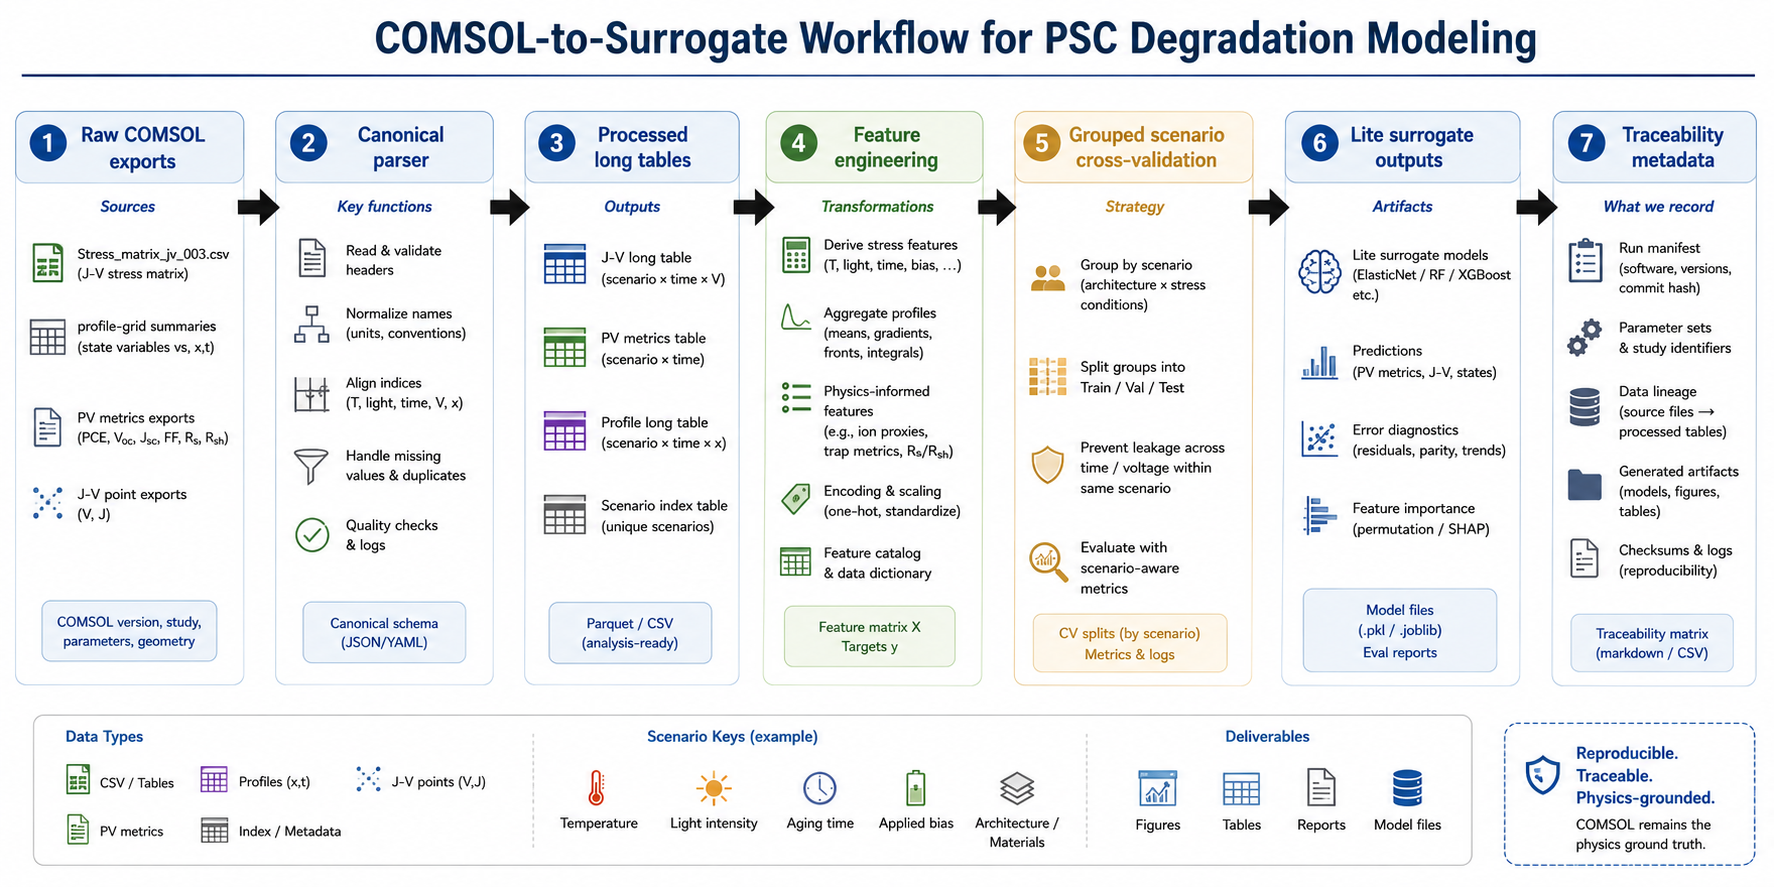
\includegraphics[width=\textwidth]{figures/ml_surrogate/comsol_to_surrogate_workflow_concept.png}
\end{minipage}\hfill
\begin{minipage}{0.49\textwidth}
\centering
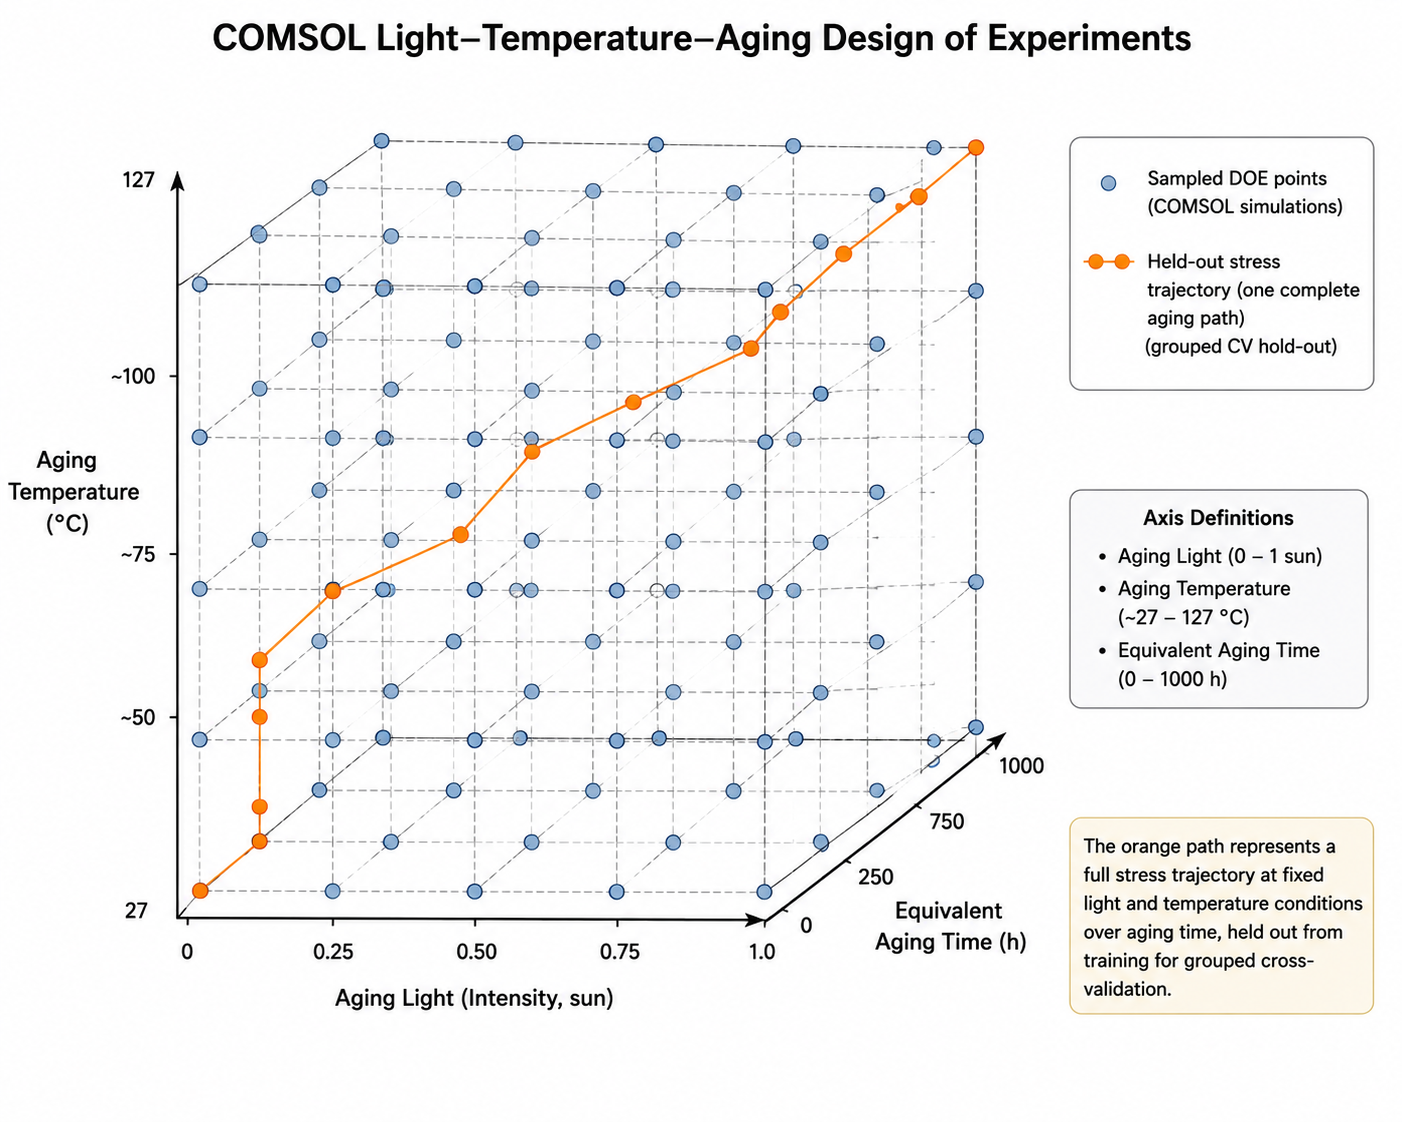
\includegraphics[width=\textwidth]{figures/ml_surrogate/aging_doe_trajectory_concept.png}
\end{minipage}
\caption[Conceptual COMSOL-to-ML workflow and design-of-experiments map.]{Conceptual schematics for the COMSOL-to-ML workflow and the
light-temperature-aging design of experiments. These panels summarize the data
contract and sampling logic; quantitative validation results are generated
separately by the reproducible surrogate scripts.}
\label{fig:ml_concept_workflow_doe}
\end{figure}

\begin{figure}[H]
\centering
\begin{minipage}{0.49\textwidth}
\centering
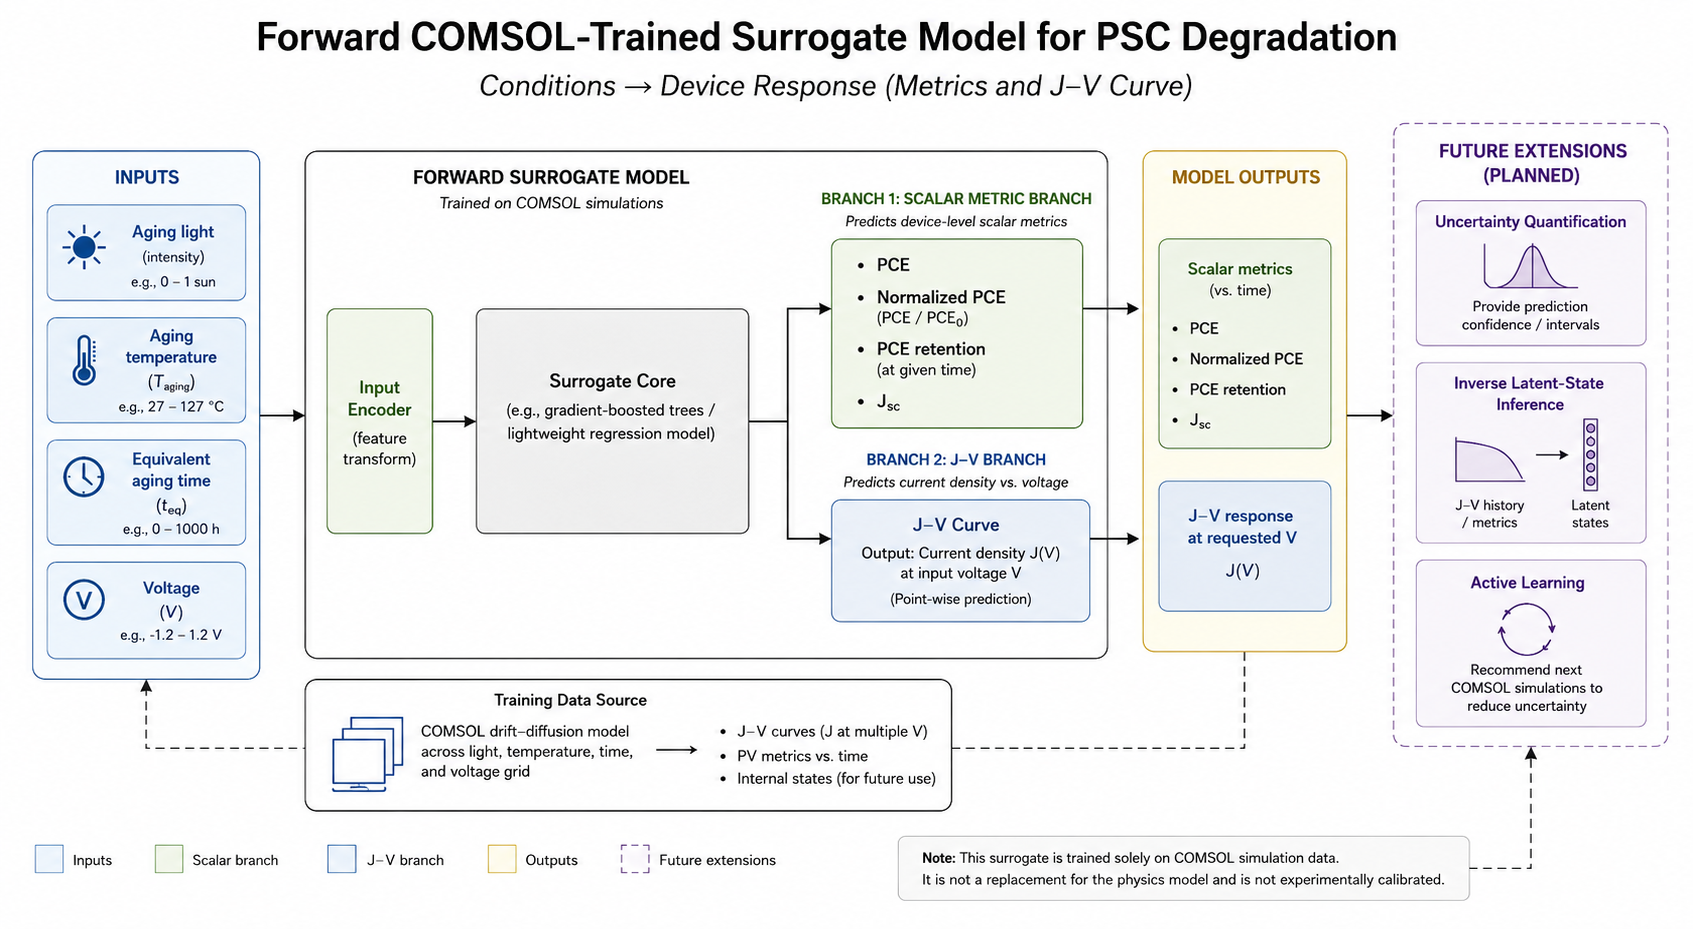
\includegraphics[width=\textwidth]{figures/ml_surrogate/forward_surrogate_architecture_concept.png}
\end{minipage}\hfill
\begin{minipage}{0.49\textwidth}
\centering
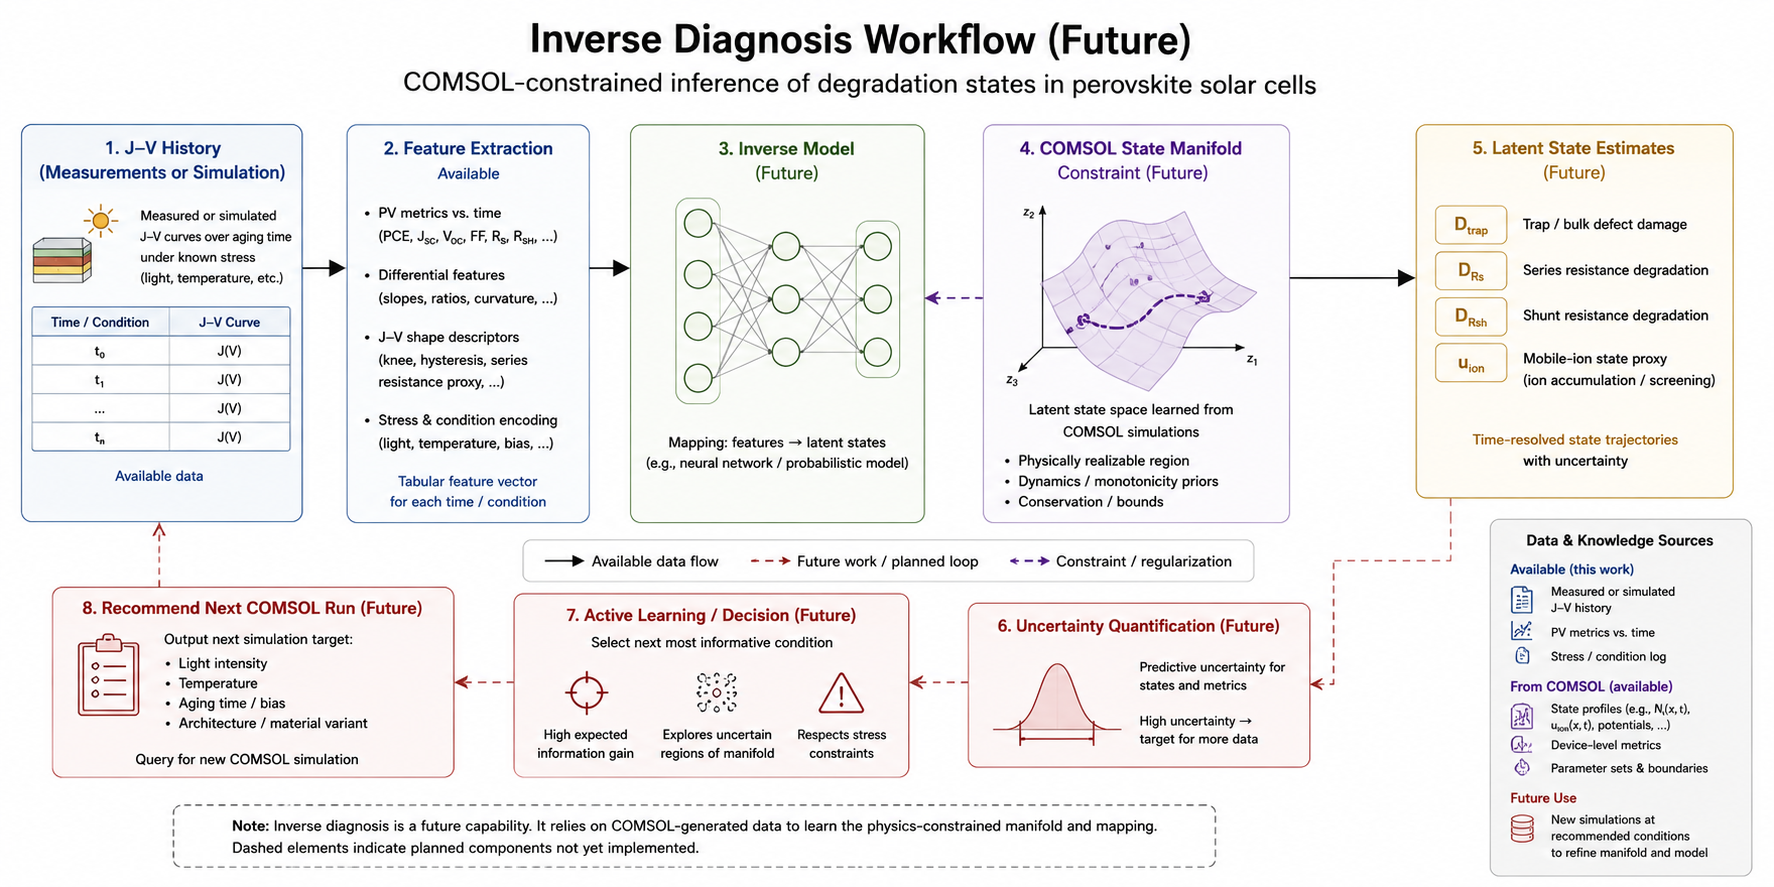
\includegraphics[width=\textwidth]{figures/ml_surrogate/inverse_diagnosis_workflow_concept.png}
\end{minipage}
\caption[Conceptual forward-surrogate and inverse-diagnosis architecture.]{Conceptual architecture diagrams for the forward COMSOL-trained
surrogate and the future inverse-diagnosis workflow. The present thesis trains
and validates the forward lite surrogate only; inverse diagnosis remains a
planned extension requiring broader COMSOL state labels and experimental
calibration.}
\label{fig:ml_concept_forward_inverse}
\end{figure}

\begin{figure}[H]
\centering
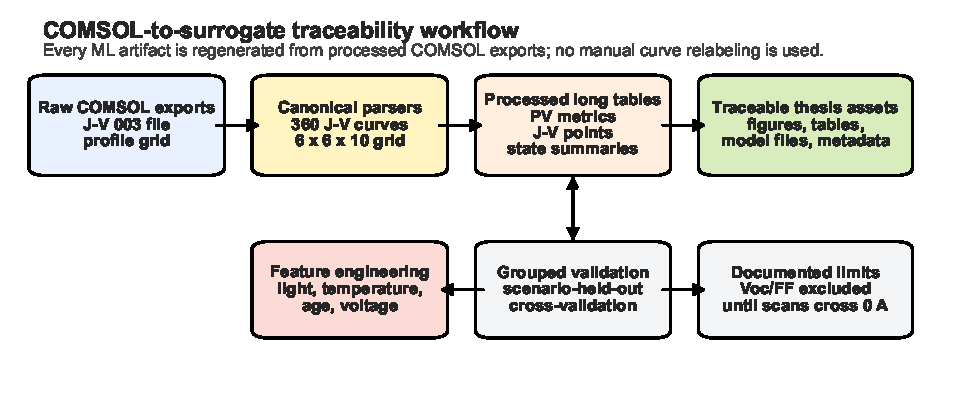
\includegraphics[width=\textwidth]{outputs/figures/surrogate_lite/surrogate_lite_data_traceability_workflow.pdf}
\caption{Traceable COMSOL-to-surrogate workflow for the lite ML baseline. The
raw flat J--V and profile-grid exports are parsed into long tables, converted
into stress, age, and voltage features, evaluated with scenario-held-out
cross-validation, and written as auditable thesis artifacts.}
\label{fig:surrogate_lite_traceability}
\end{figure}

The current ML-ready data set contains 36 light-temperature scenarios, ten
aging checkpoints per scenario, and 48 voltage samples per J--V curve, giving
360 diagnostic curves and 17,280 current-density points. The profile-grid
summary contributes 2520 internal-state rows across seven exported variables.
The voltage sweep ends at 1.25 V, so only 115 of the 360 curves have resolved
zero-current crossings. For this reason, $V_{oc}$ and FF are excluded from the
lite surrogate targets until the diagnostic voltage range is extended. The
trained scalar targets are PCE, normalized PCE, PCE retention, and $J_{sc}$;
the curve target is current density $J(V)$.

\begin{table}[H]
\centering
\caption{Grouped scenario cross-validation metrics for the lite COMSOL-trained surrogate baseline. Scenario grouping keeps complete light-temperature aging trajectories out of the training fold before prediction.}
\label{tab:surrogate_lite_cv_metrics}
\begin{tabular}{@{}lrrrr@{}}
\toprule
Target & Samples & Groups & MAE & $R^2$ \\
\midrule
PCE (%) & 360 & 36 & 0.393 & 0.884 \\
Normalized PCE $(\mathrm{PCE}/\mathrm{PCE}_0)$ & 360 & 36 & 0.0174 & 0.884 \\
PCE retention (%) & 360 & 36 & 1.74 & 0.884 \\
$J_{sc}$ (mA cm$^{-2}$) & 360 & 36 & 0.0767 & 0.864 \\
$J(V)$ (mA cm$^{-2}$) & 17280 & 36 & 0.286 & 0.955 \\
\bottomrule
\end{tabular}
\end{table}


\begin{figure}[H]
\centering
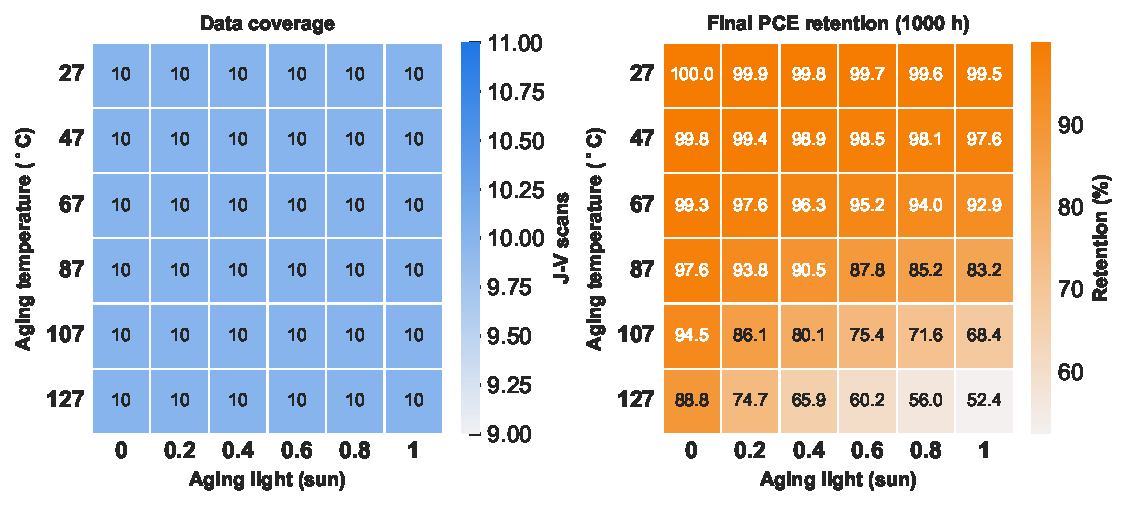
\includegraphics[width=0.95\textwidth]{outputs/figures/surrogate_lite/surrogate_lite_doe_coverage.pdf}
\caption{Design-of-experiments coverage and final degradation surface used for
the lite surrogate. Each light-temperature scenario has ten diagnostic J--V
curves, and the final PCE-retention surface spans near-unity retention at low
stress to 52.4\% at 400 K and one sun.}
\label{fig:surrogate_lite_doe_coverage}
\end{figure}

\begin{figure}[H]
\centering
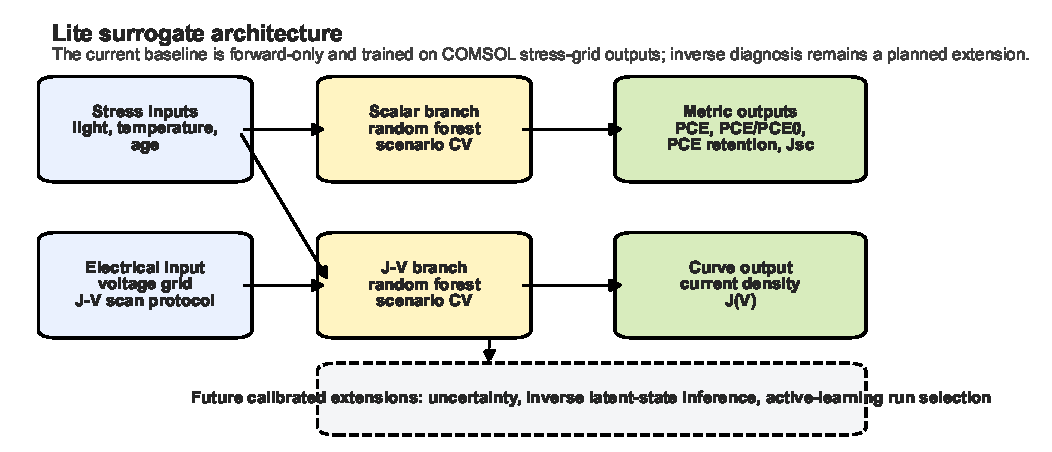
\includegraphics[width=\textwidth]{outputs/figures/surrogate_lite/surrogate_lite_model_architecture.pdf}
\caption{Forward surrogate architecture used for the lite baseline. Stress and
age features feed scalar photovoltaic metric models, while stress, age, and
voltage feed the J--V current-density model. Uncertainty, inverse diagnosis,
and active learning remain planned calibrated extensions.}
\label{fig:surrogate_lite_architecture}
\end{figure}

The validation split is grouped by \texttt{scenario\_index}. Entire
light-temperature aging trajectories are held out by fold rather than randomly
mixing rows from the same scenario into training and test sets. This is a more
conservative test of interpolation across stress space. Table
\ref{tab:surrogate_lite_cv_metrics} shows that the first baseline already
predicts PCE retention with 1.74 percentage-point MAE and predicts
current-density points with $0.286~\mathrm{mA/cm^2}$ MAE. The scalar $R^2$
values are about 0.86--0.88, while the J--V current-density model reaches
$R^2=0.955$. These values are promising for a lightweight surrogate, but they
should be interpreted as COMSOL-to-COMSOL interpolation accuracy, not
experimental prediction accuracy.

\begin{figure}[H]
\centering
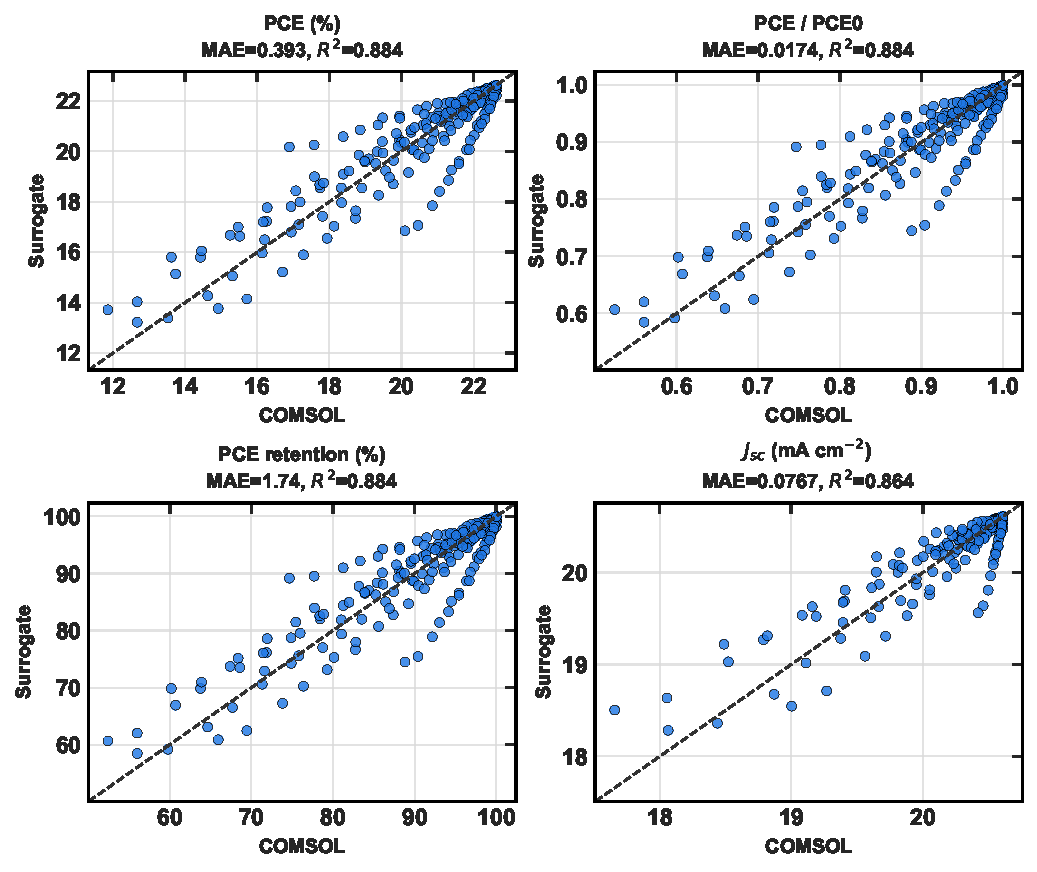
\includegraphics[width=0.92\textwidth]{outputs/figures/surrogate_lite/surrogate_lite_actual_vs_pred.pdf}
\caption{Scenario-held-out COMSOL versus lite-surrogate predictions for scalar
photovoltaic targets. The diagonal line is the ideal one-to-one response.}
\label{fig:surrogate_lite_actual_vs_pred}
\end{figure}

\begin{figure}[H]
\centering
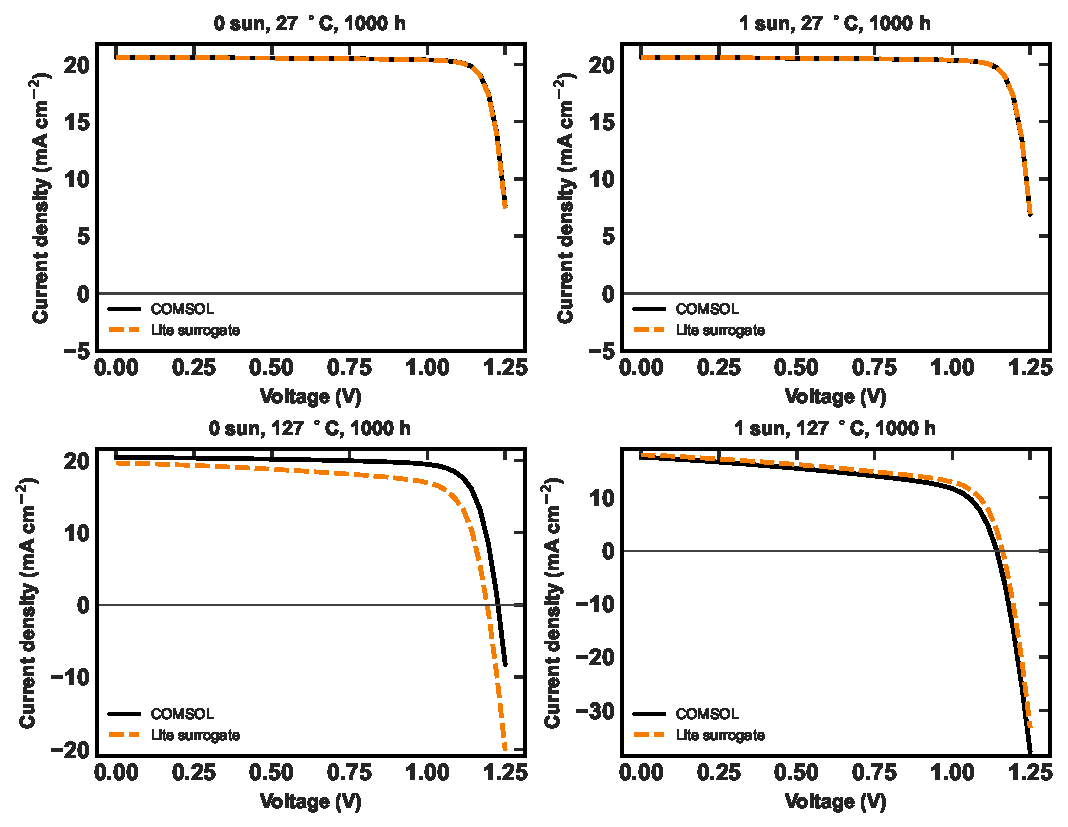
\includegraphics[width=0.92\textwidth]{outputs/figures/surrogate_lite/surrogate_lite_jv_group_cv_examples.pdf}
\caption[Scenario-held-out J--V examples for the lite surrogate.]{Representative scenario-held-out J--V predictions at the four
light-temperature stress corners after 1000 h equivalent aging. The
low-stress corners remain close to the COMSOL curves, while the high-temperature
corners expose the largest interpolation errors near the knee and zero-current
region.}
\label{fig:surrogate_lite_jv_examples}
\end{figure}

\begin{figure}[H]
\centering
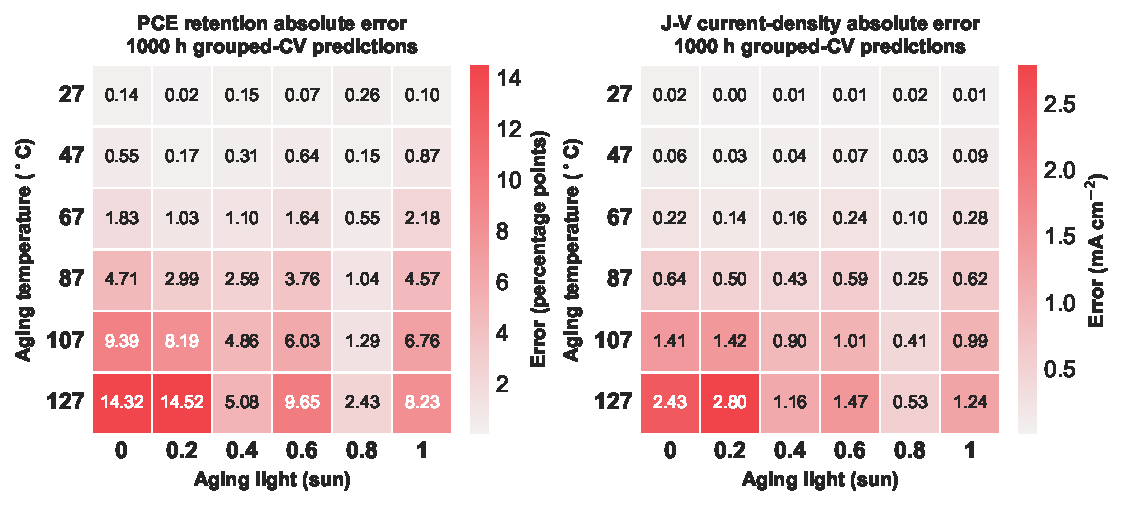
\includegraphics[width=0.95\textwidth]{outputs/figures/surrogate_lite/surrogate_lite_error_maps.pdf}
\caption{Final-age absolute-error maps from the grouped cross-validation
predictions. The largest PCE-retention errors occur at the highest-temperature
edge of the stress grid, identifying where additional COMSOL simulations or a
more structured surrogate would be most useful.}
\label{fig:surrogate_lite_error_maps}
\end{figure}

\begin{figure}[H]
\centering
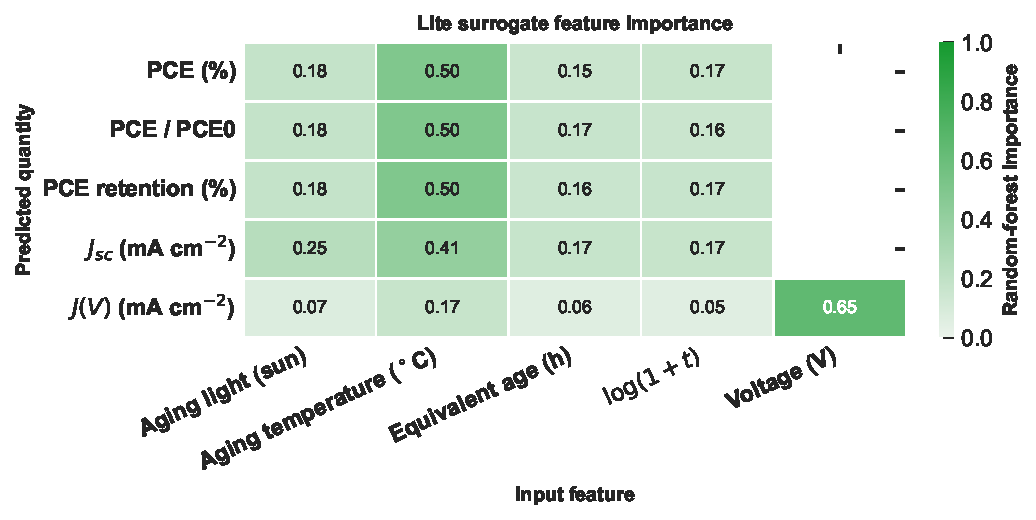
\includegraphics[width=0.86\textwidth]{outputs/figures/surrogate_lite/surrogate_lite_feature_importance.pdf}
\caption{Random-forest feature importances for the final lite surrogate models.
Temperature dominates the scalar degradation targets in this COMSOL export,
while voltage dominates the J--V current-density branch as expected.}
\label{fig:surrogate_lite_feature_importance}
\end{figure}

\begin{figure}[H]
\centering
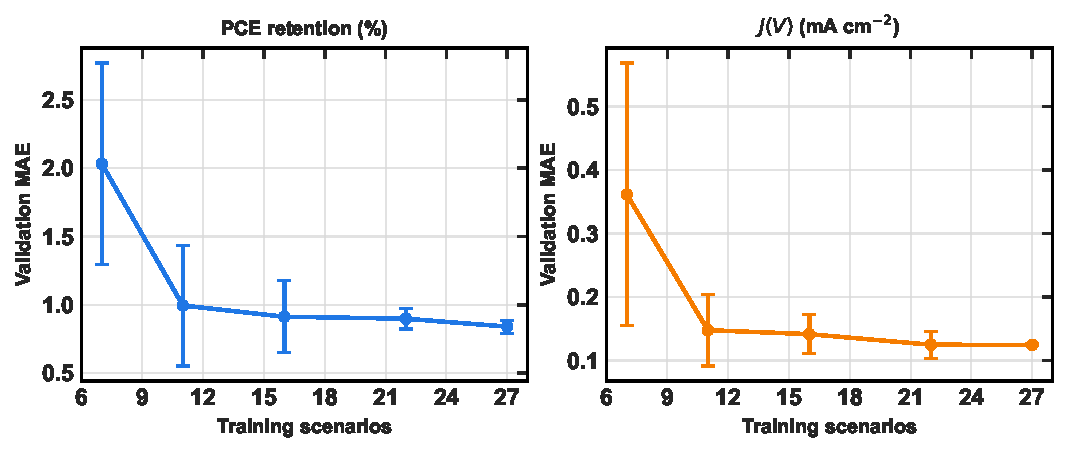
\includegraphics[width=0.84\textwidth]{outputs/figures/surrogate_lite/surrogate_lite_learning_curve.pdf}
\caption{Training-size sensitivity for the lite surrogate. The validation MAE
drops rapidly after the smallest training subsets and then begins to plateau,
indicating that the existing grid is enough for a first baseline but not enough
to replace calibrated COMSOL sweeps.}
\label{fig:surrogate_lite_learning_curve}
\end{figure}

The ML result is therefore a useful thesis support result. It proves that the
COMSOL exports can be converted into a reproducible surrogate-ready data set,
that grouped validation is possible without manual relabeling, and that the
largest residuals can be traced back to specific stress regions. The remaining
gap is calibration and breadth: future work should add more architectures,
complete voltage windows for $V_{oc}$ and FF, repeated COMSOL samples for
uncertainty, and matched experimental aging data before the surrogate is used
for inverse diagnosis or field prediction.

\section{Current Data-Quality Gaps}

The canonical light-temperature stress-matrix J--V result in this thesis is
\path{data/raw/comsol/arch_baseline_pin/Aging/Stress_matrix_jv_003.csv}. Earlier
exports, \path{Stress_matrix_jv_001.csv} and \path{Stress_matrix_jv_002.csv},
are retained only as superseded development history. They are useful for
auditing the export evolution, but they should not be interpreted as missing
low-light data or as parallel quantitative results. The current remaining
data-quality limitation is instead the voltage range of the canonical
\path{Stress_matrix_jv_003.csv} export: many mild or early-aging curves do not
cross zero current by 1.25 V. Therefore PCE and $J_{sc}$ are available for the
full 360-curve grid, while $V_{oc}$ and FF are complete only for the subset of
curves with a resolved zero-current crossing. A future diagnostic sweep to
approximately 1.45 V would make $V_{oc}$ and FF complete across the full
light-temperature grid.

\section{Hysteresis Result}

\begin{figure}[H]
\centering
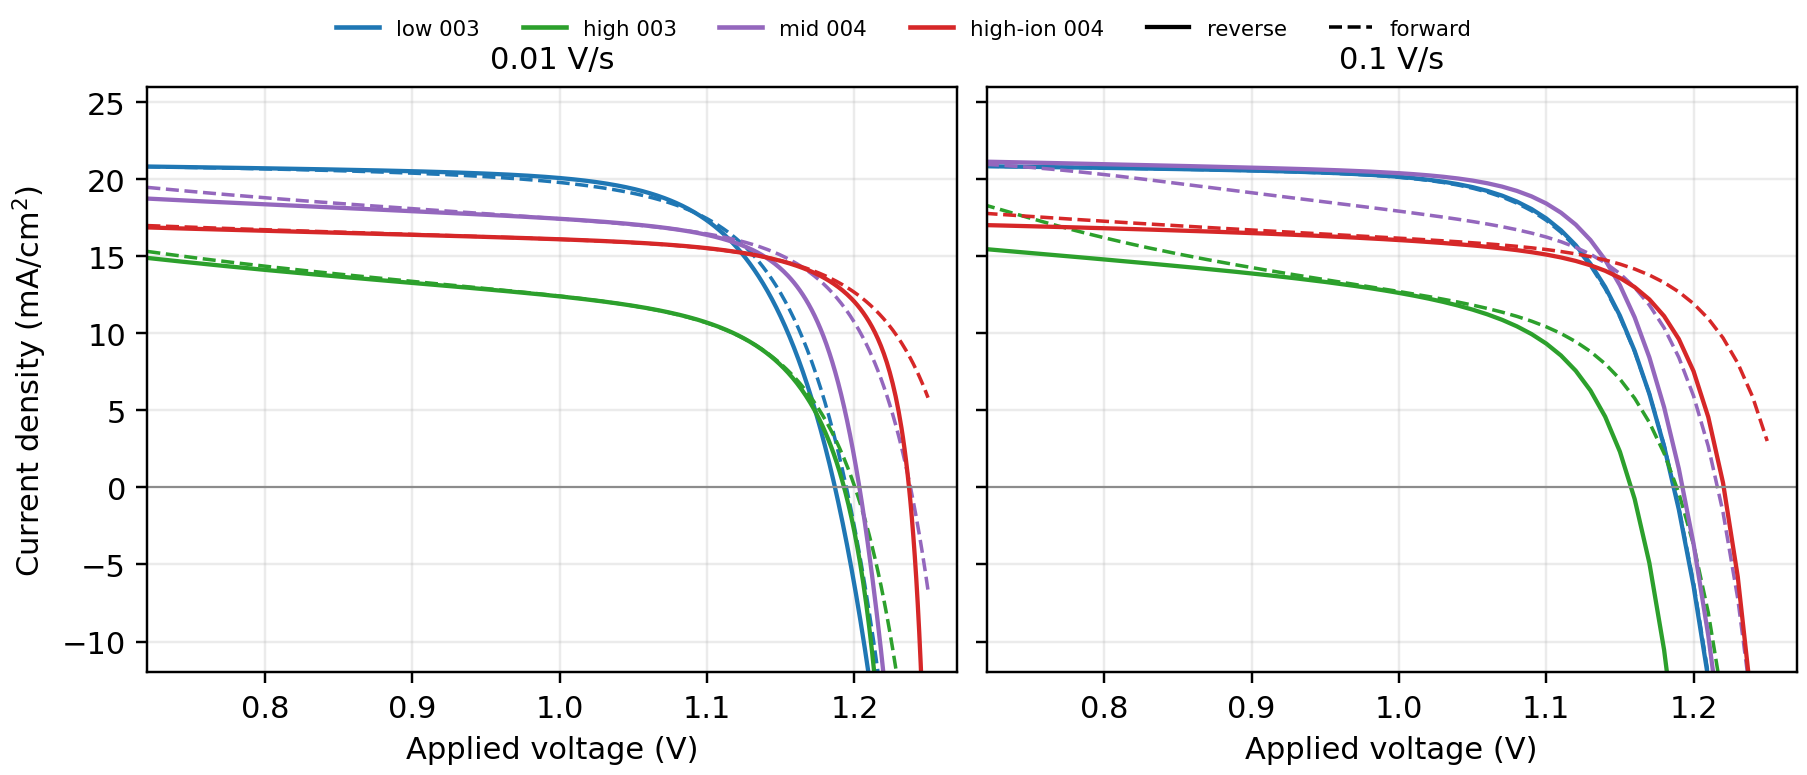
\includegraphics[width=0.78\textwidth]{figures/eee598_comsol/jv_curves.png}
\caption{Forward and reverse J--V scans from the COMSOL hysteresis protocol.}
\label{fig:results_hysteretic_jv}
\end{figure}

Figure~\ref{fig:results_hysteretic_jv} shows scan-direction-dependent J--V
behavior. The variable that changes during the scan is the normalized ion state
$u_{\mathrm{ion}}$. Through Eq.~\ref{eq:rho_ion}, ion redistribution modifies
the electrostatic source term. As ions accumulate near one interface and
deplete near the opposite side, the internal charge distribution changes,
altering band bending and shifting the measured J--V curve depending on scan
history. The result supports the physical need for time-dependent scan
simulation. This presentation case uses
$N_0=10^{17}~\mathrm{cm^{-3}}$,
$\mu_{\mathrm{ion}}=10^{-18}~\mathrm{m^2/(V\,s)}$, and
$r_{\mathrm{scan}}=0.1~\mathrm{V/s}$. It is a separate presentation diagnostic
case rather than part of the canonical
\path{Stress_matrix_jv_003.csv} light-temperature grid, and it does not prove
that the selected ion mobility or concentration is unique.

\section{Spatial and Transient Validation Results}

The newest COMSOL profile exports include the band-edge and quasi-Fermi-level
variables needed to check the simulated internal electrostatics. The selected
band-diagram cases in Fig.~\ref{fig:band_diagrams_selected_cases} use the
native left-to-right COMSOL coordinate, with the HTL side on the left and the
ETL side on the right. Energies were exported by COMSOL as joules and converted
to electron-volts for plotting. The resulting profiles show a monotonic
internal band-bending trend across the absorber and carrier-selective
alignment at the transport-layer sides. These plots do not replace a full
operating-point validation at short circuit, maximum power, and open circuit,
but they remove the previous coordinate-direction ambiguity.

\begin{figure}[H]
\centering
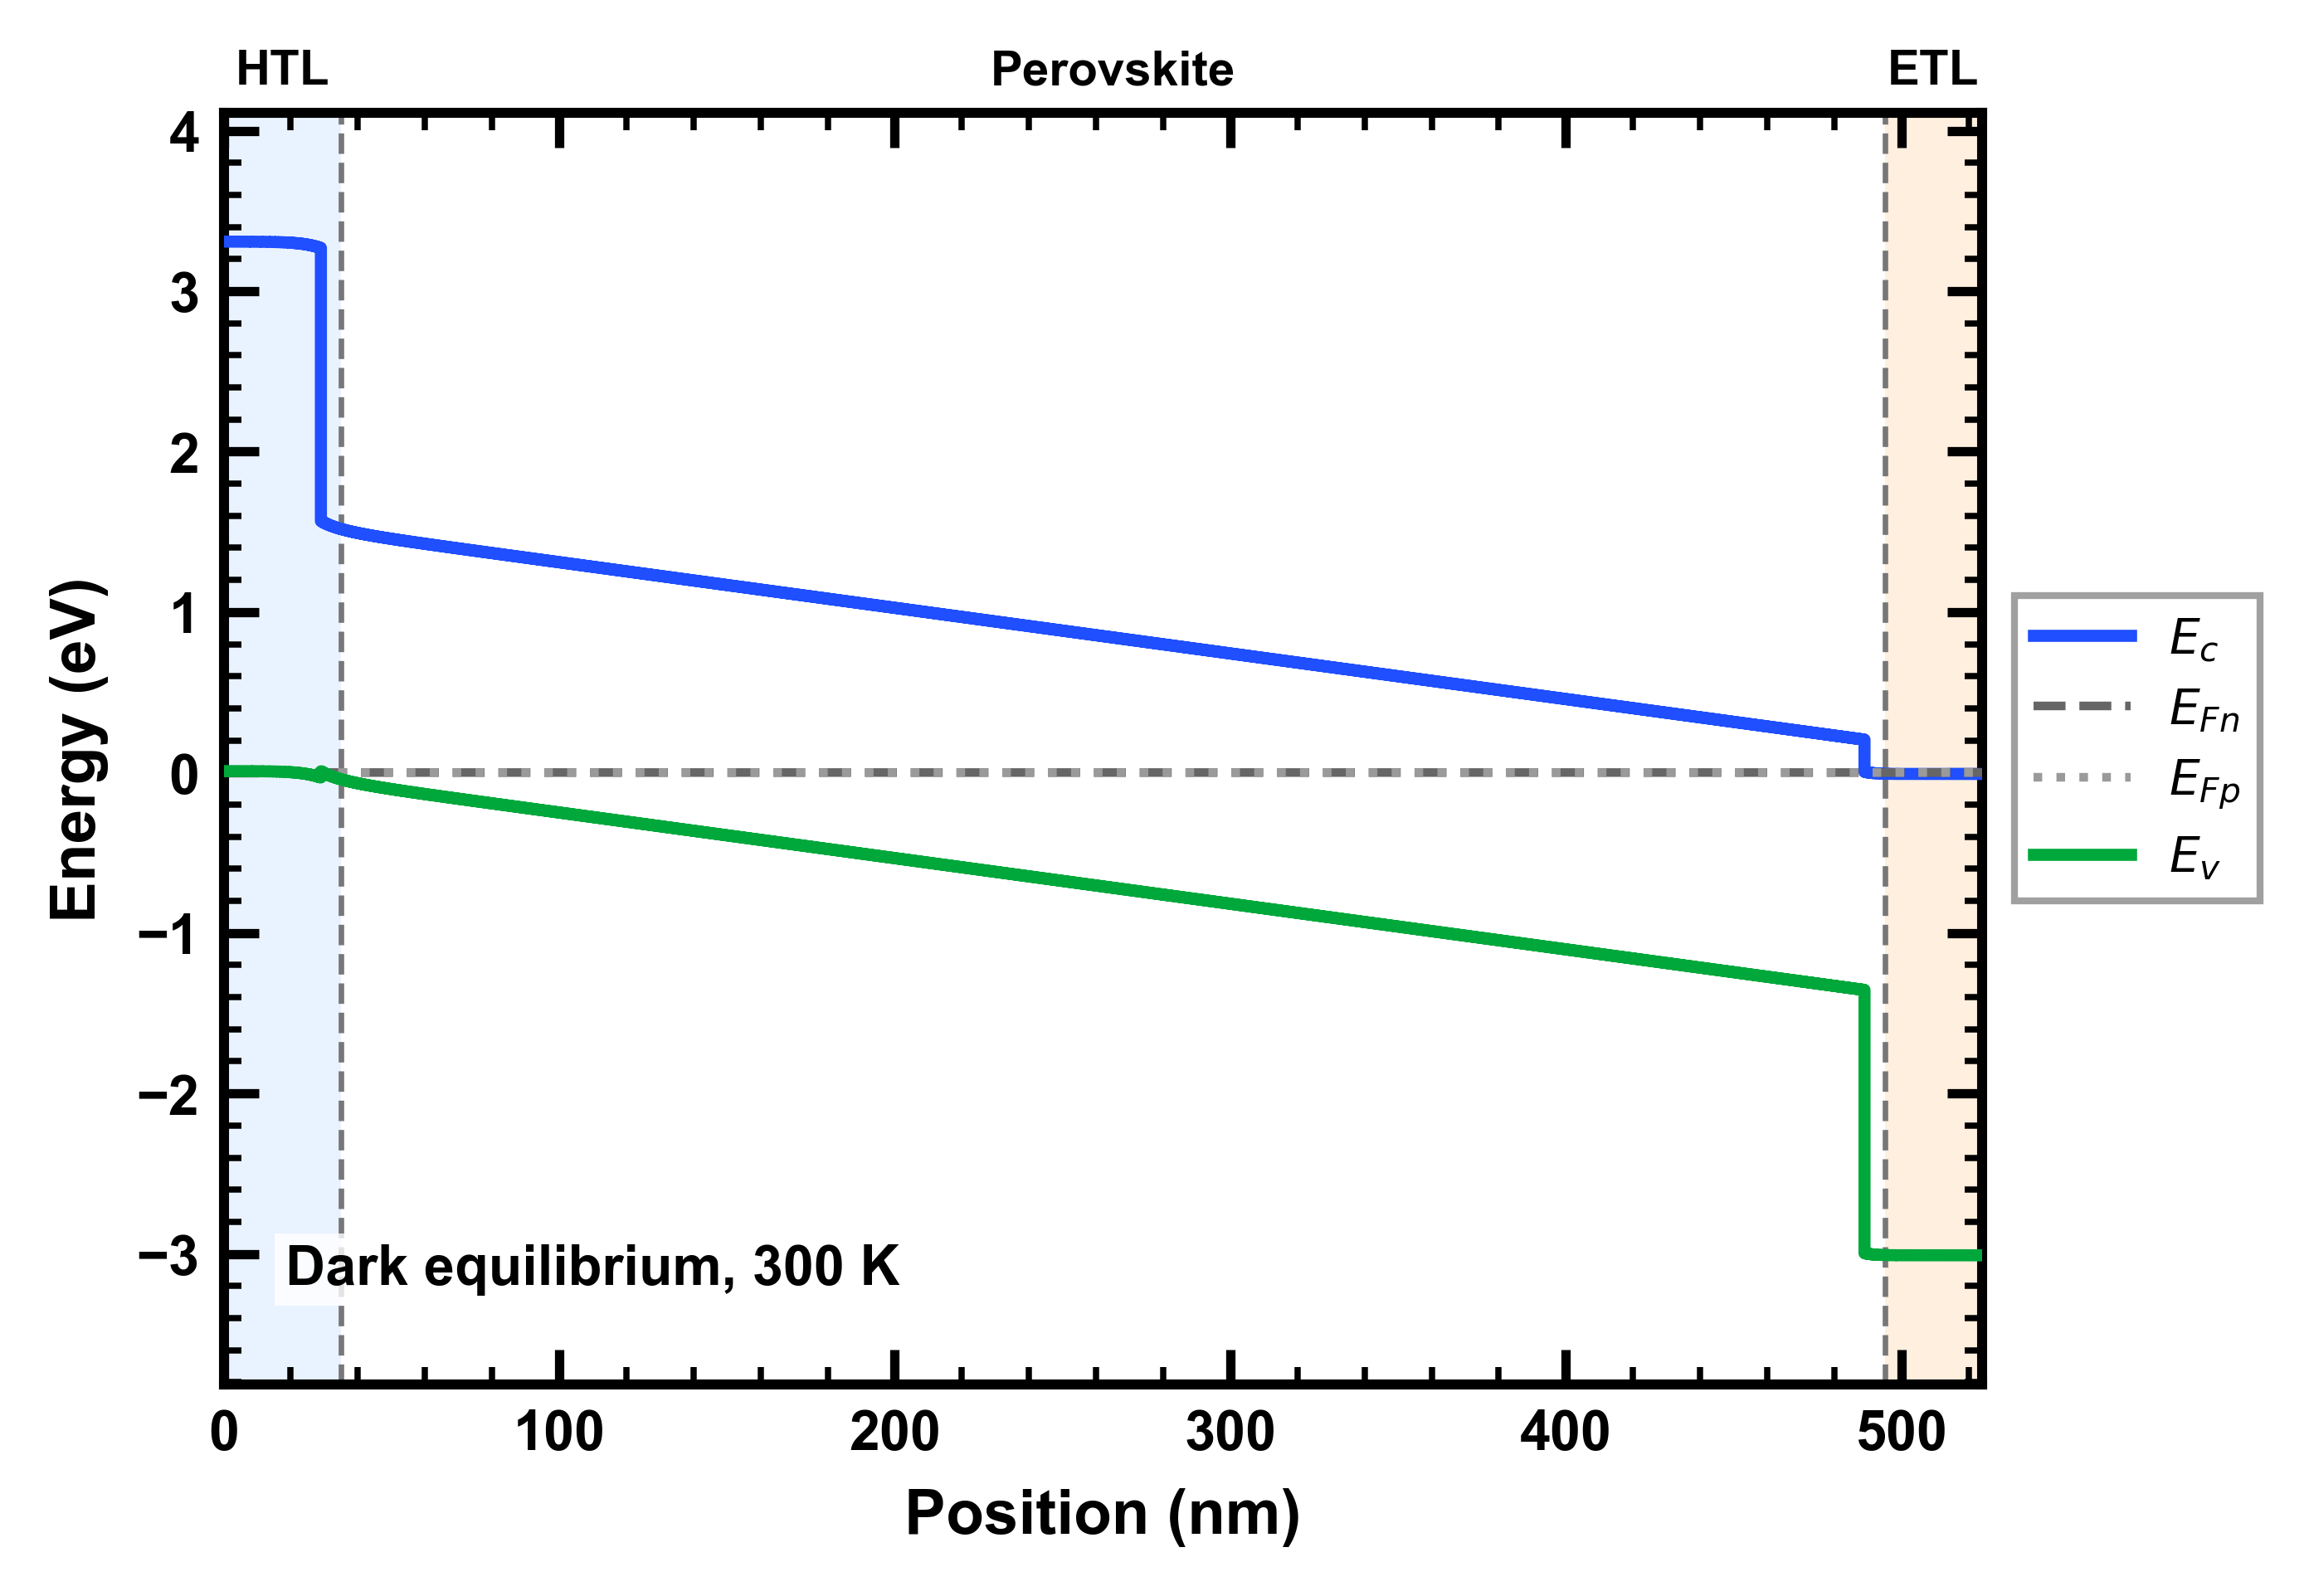
\includegraphics[width=0.76\textwidth]{outputs/figures/comsol_architecture_stress_grid/baseline_pin_band_diagram_dark_equilibrium_300K.png}
\caption{COMSOL dark-equilibrium band diagram for the 300 K baseline device.
This figure is generated from the dedicated equilibrium energy-level export,
not from the low-light aging grid. The electron and hole quasi-Fermi levels
overlap to numerical precision, as expected for a true equilibrium solution.
The native coordinate is preserved, with the HTL on the left and the ETL on the
right.}
\label{fig:band_diagram_dark_equilibrium_300k}
\end{figure}

\begin{figure}[H]
\centering
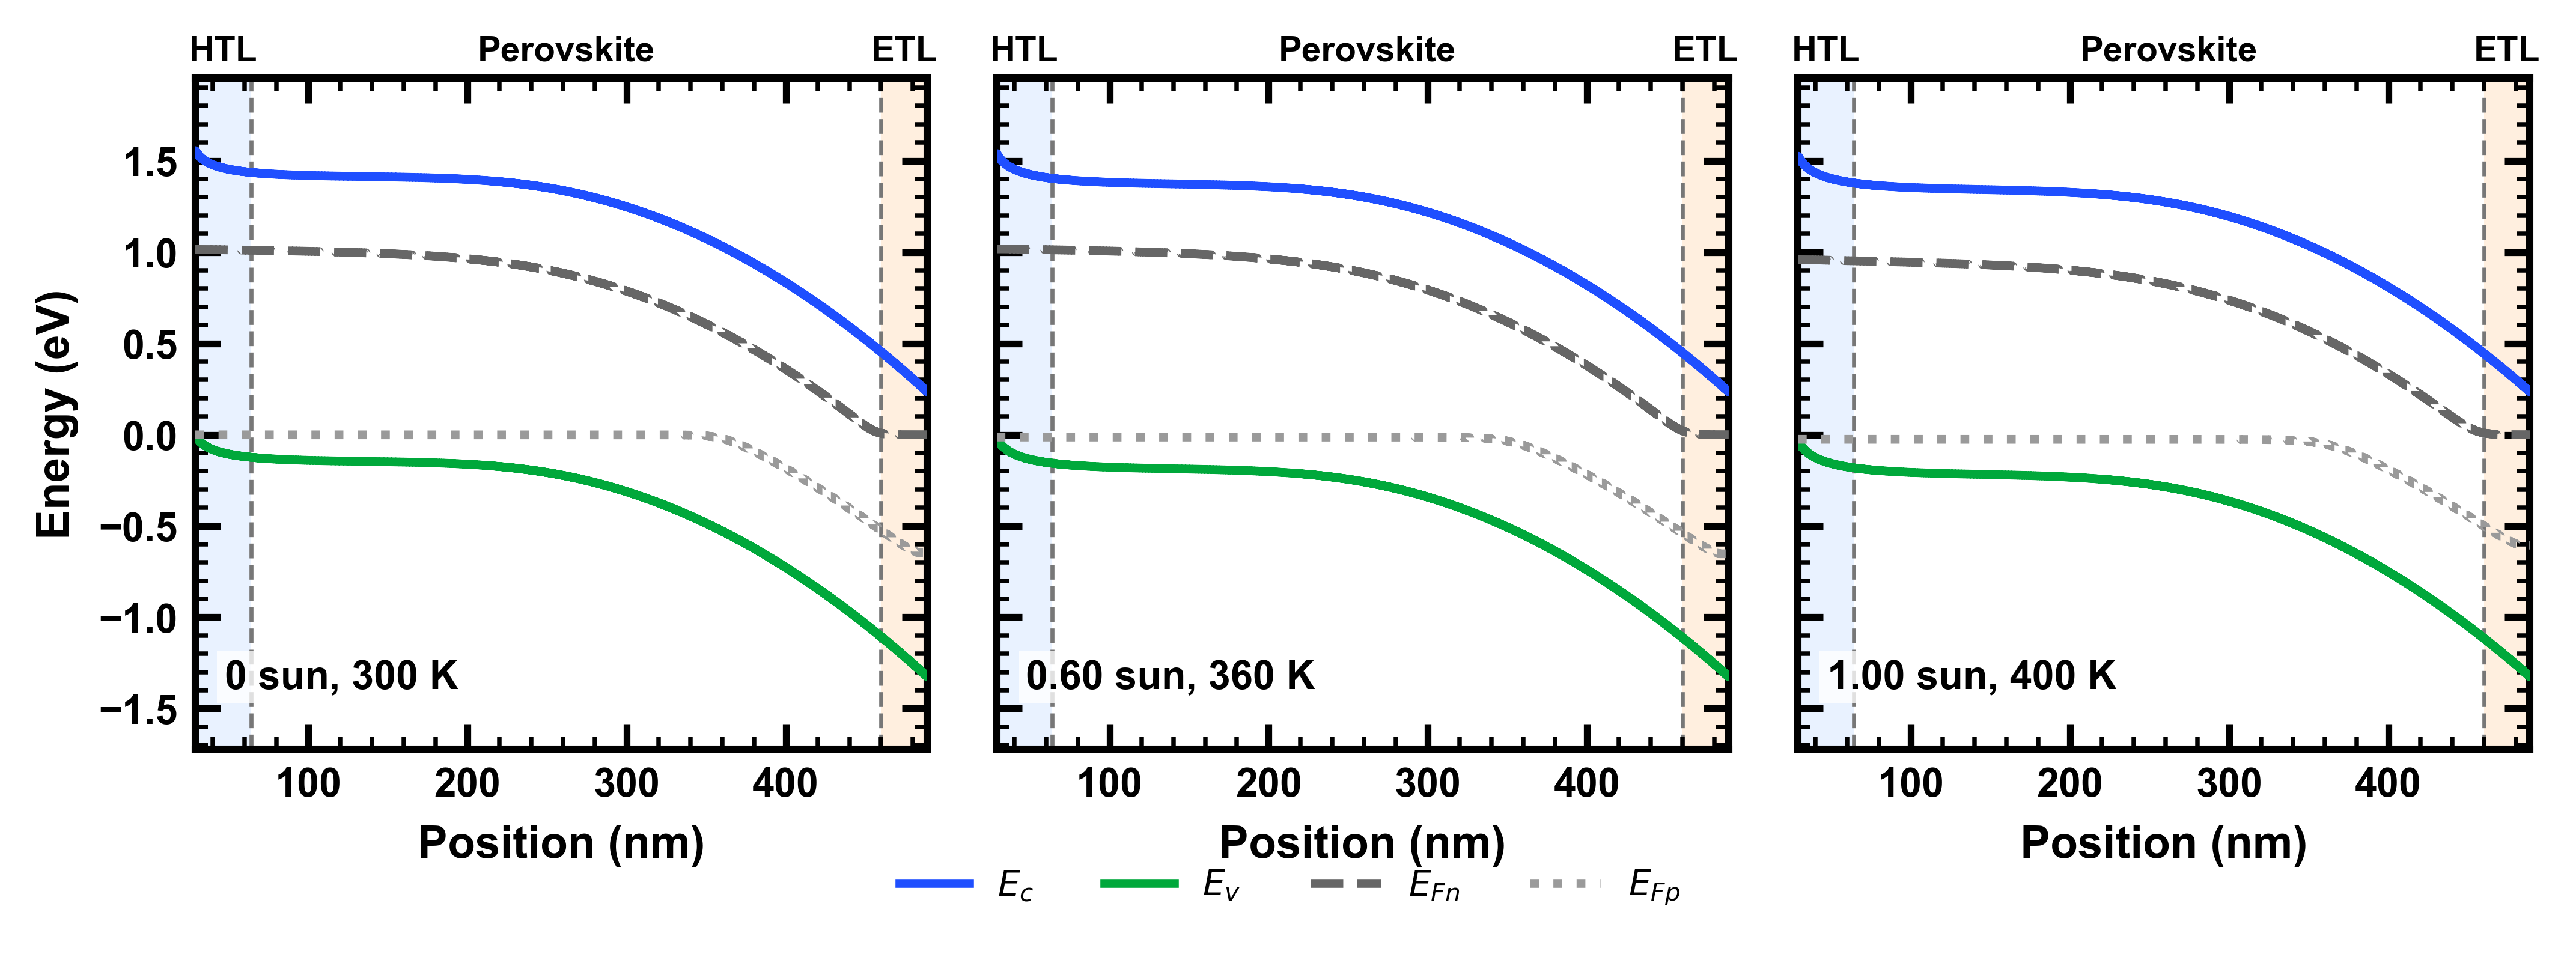
\includegraphics[width=\textwidth]{outputs/figures/comsol_architecture_stress_grid/baseline_pin_band_diagrams_selected_cases.png}
\caption{Selected COMSOL band diagrams from the newest aging-profile exports.
The panels compare final 1000 h profiles for representative low-, medium-, and
high-stress cases. The shaded regions identify the HTL side, perovskite
absorber, and ETL side without reversing the exported coordinate.}
\label{fig:band_diagrams_selected_cases}
\end{figure}

The profile-grid summary in Fig.~\ref{fig:profile_grid_final_state_summary}
establishes that the internal state variables can be exported and summarized
across stress conditions. Figures~\ref{fig:spatial_profiles_selected_cases}
and~\ref{fig:spatial_profiles_high_stress} use those same exports to show the
spatial form of the ion, trap, effective trap-density, and electric-field
states directly. These profiles support the qualitative interpretation that
aging is spatially localized near the transport-layer interfaces, with the
largest trap-density response under combined high light and high temperature.
The perovskite-domain average of $u_{\mathrm{ion}}$ in
Table~\ref{tab:spatial_profile_summary} is included as a normalization
diagnostic; strict ion conservation should be checked with the same COMSOL
integration operator used in the model.

\begin{figure}[H]
\centering
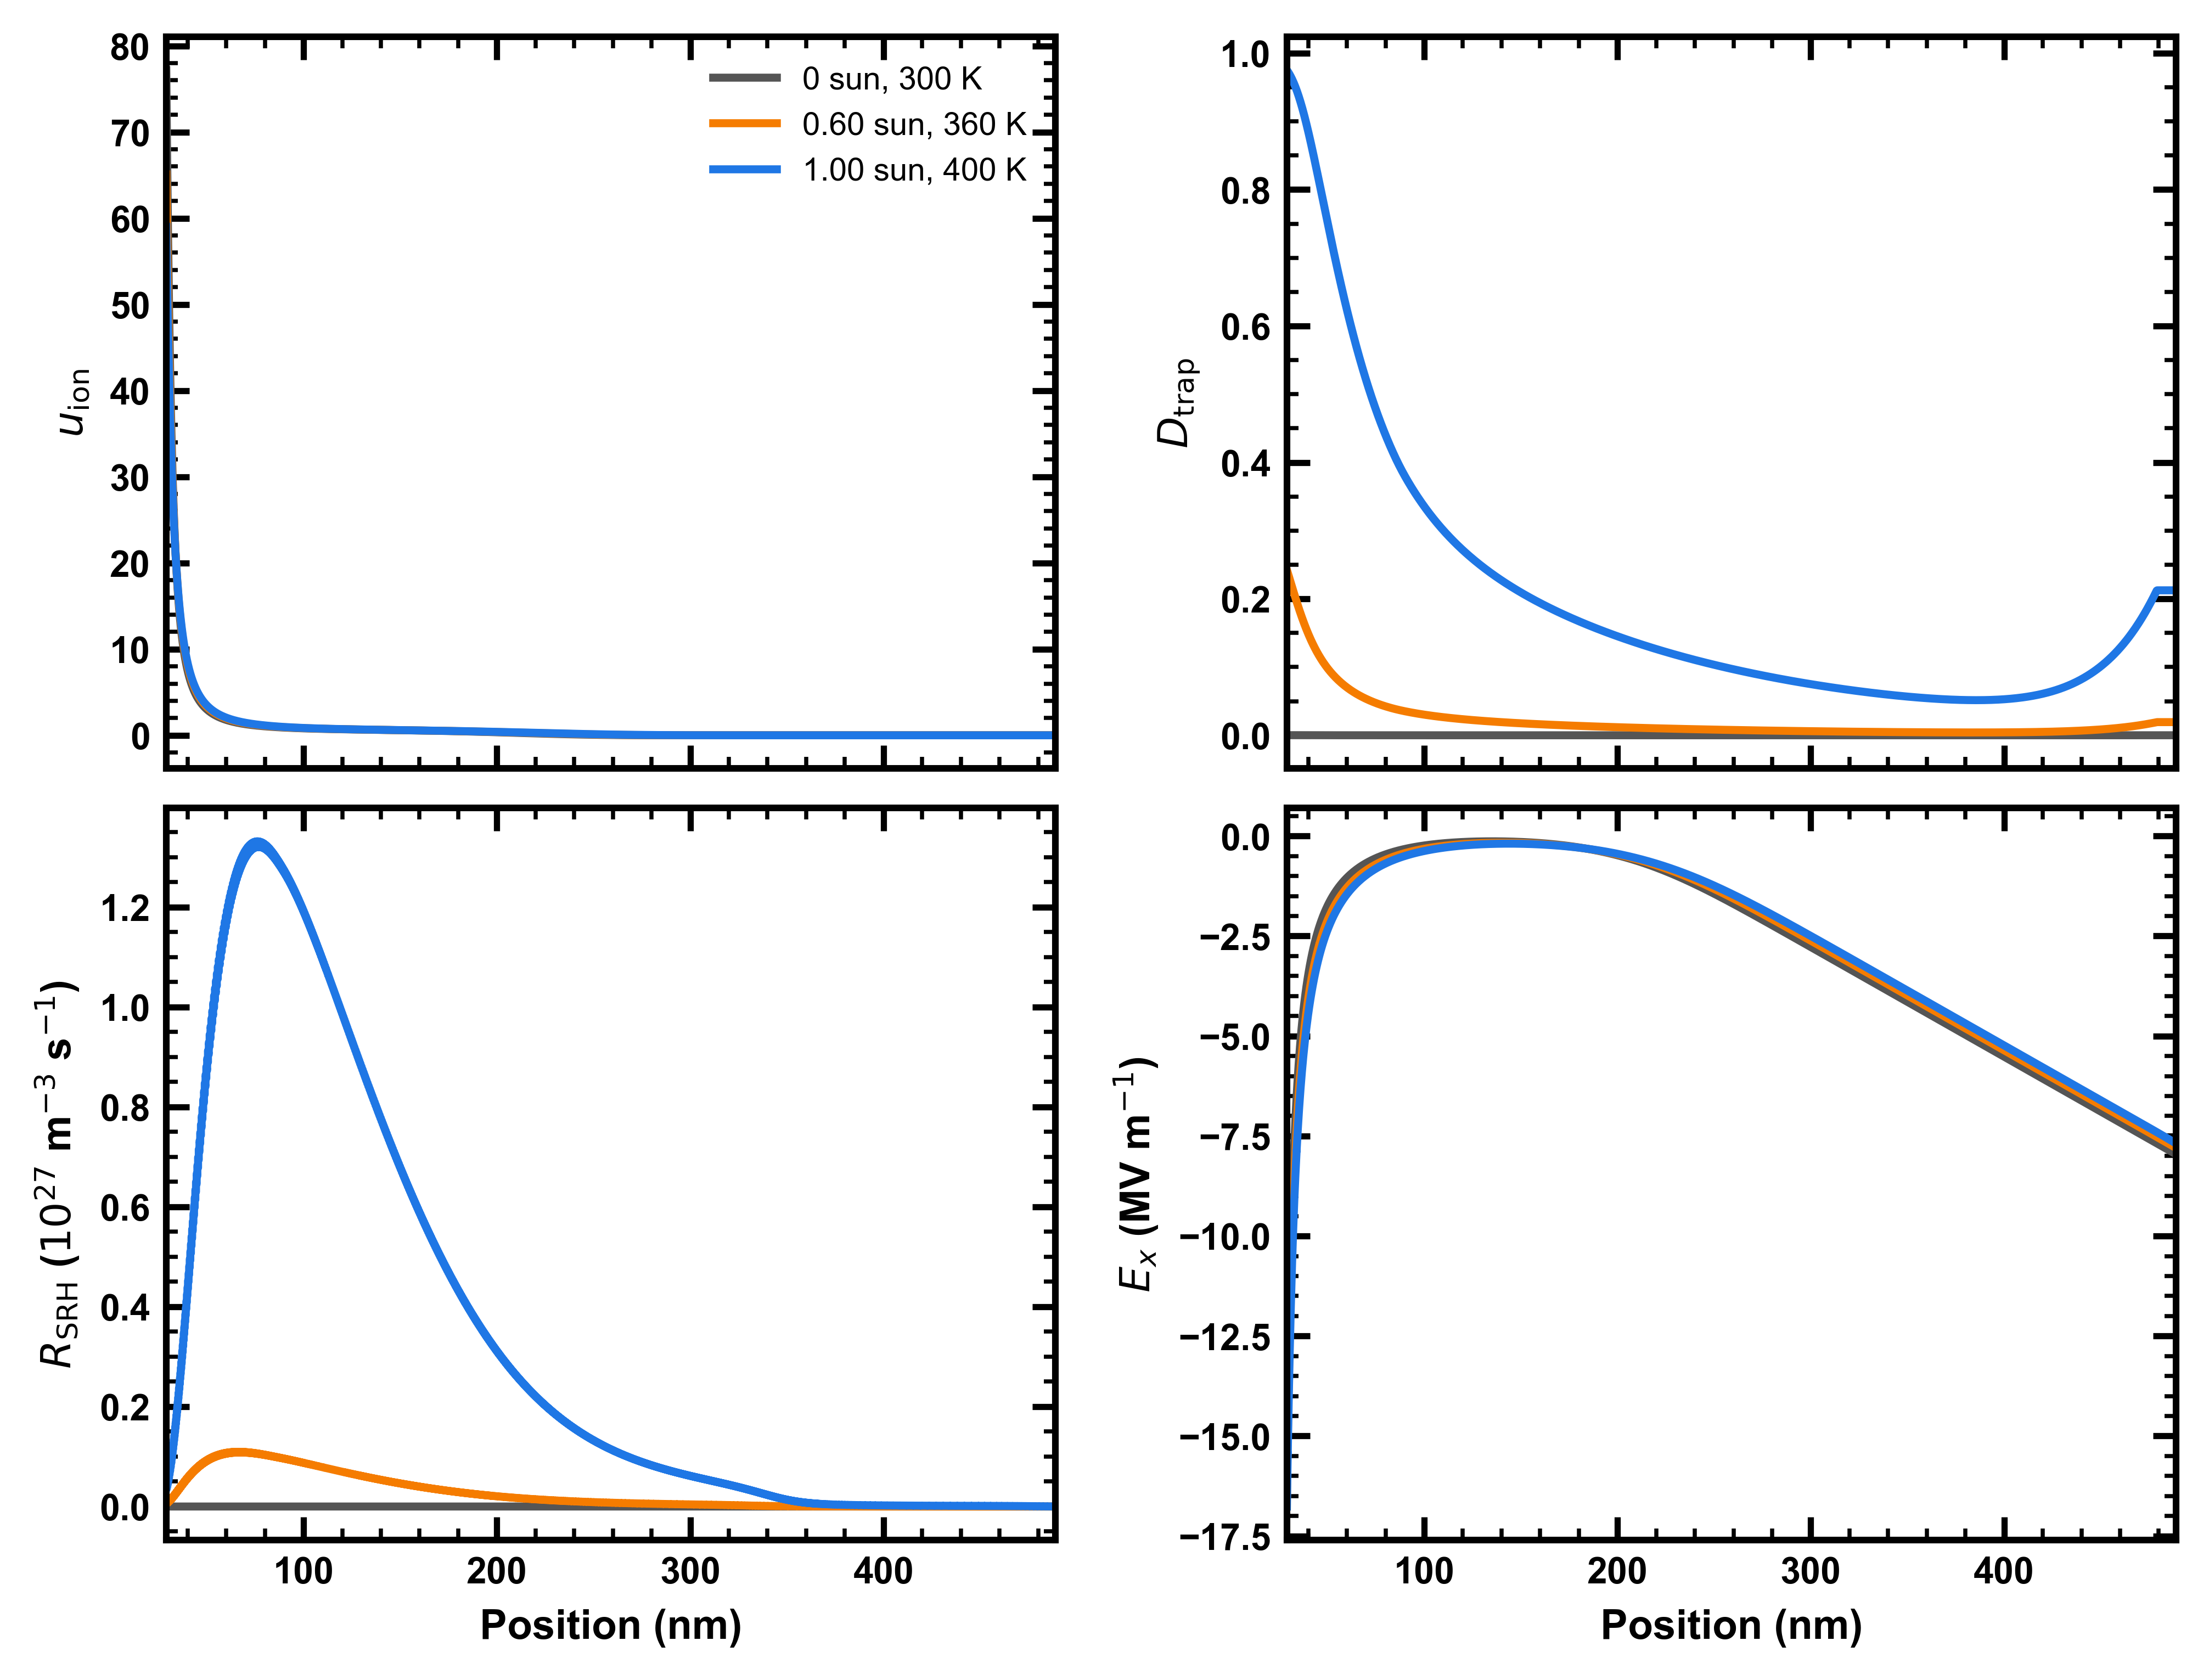
\includegraphics[width=0.92\textwidth]{outputs/figures/comsol_architecture_stress_grid/baseline_pin_spatial_profiles_selected_cases.png}
\caption{Selected final-state spatial profiles from the baseline p-i-n
light-temperature grid. The panels compare low-, medium-, and high-stress
cases at 1000 h equivalent aging for normalized ion concentration, latent trap
damage, effective trap density, and electric field. Shaded regions identify
the HTL and ETL sides without reversing the COMSOL coordinate.}
\label{fig:spatial_profiles_selected_cases}
\end{figure}

\begin{figure}[H]
\centering
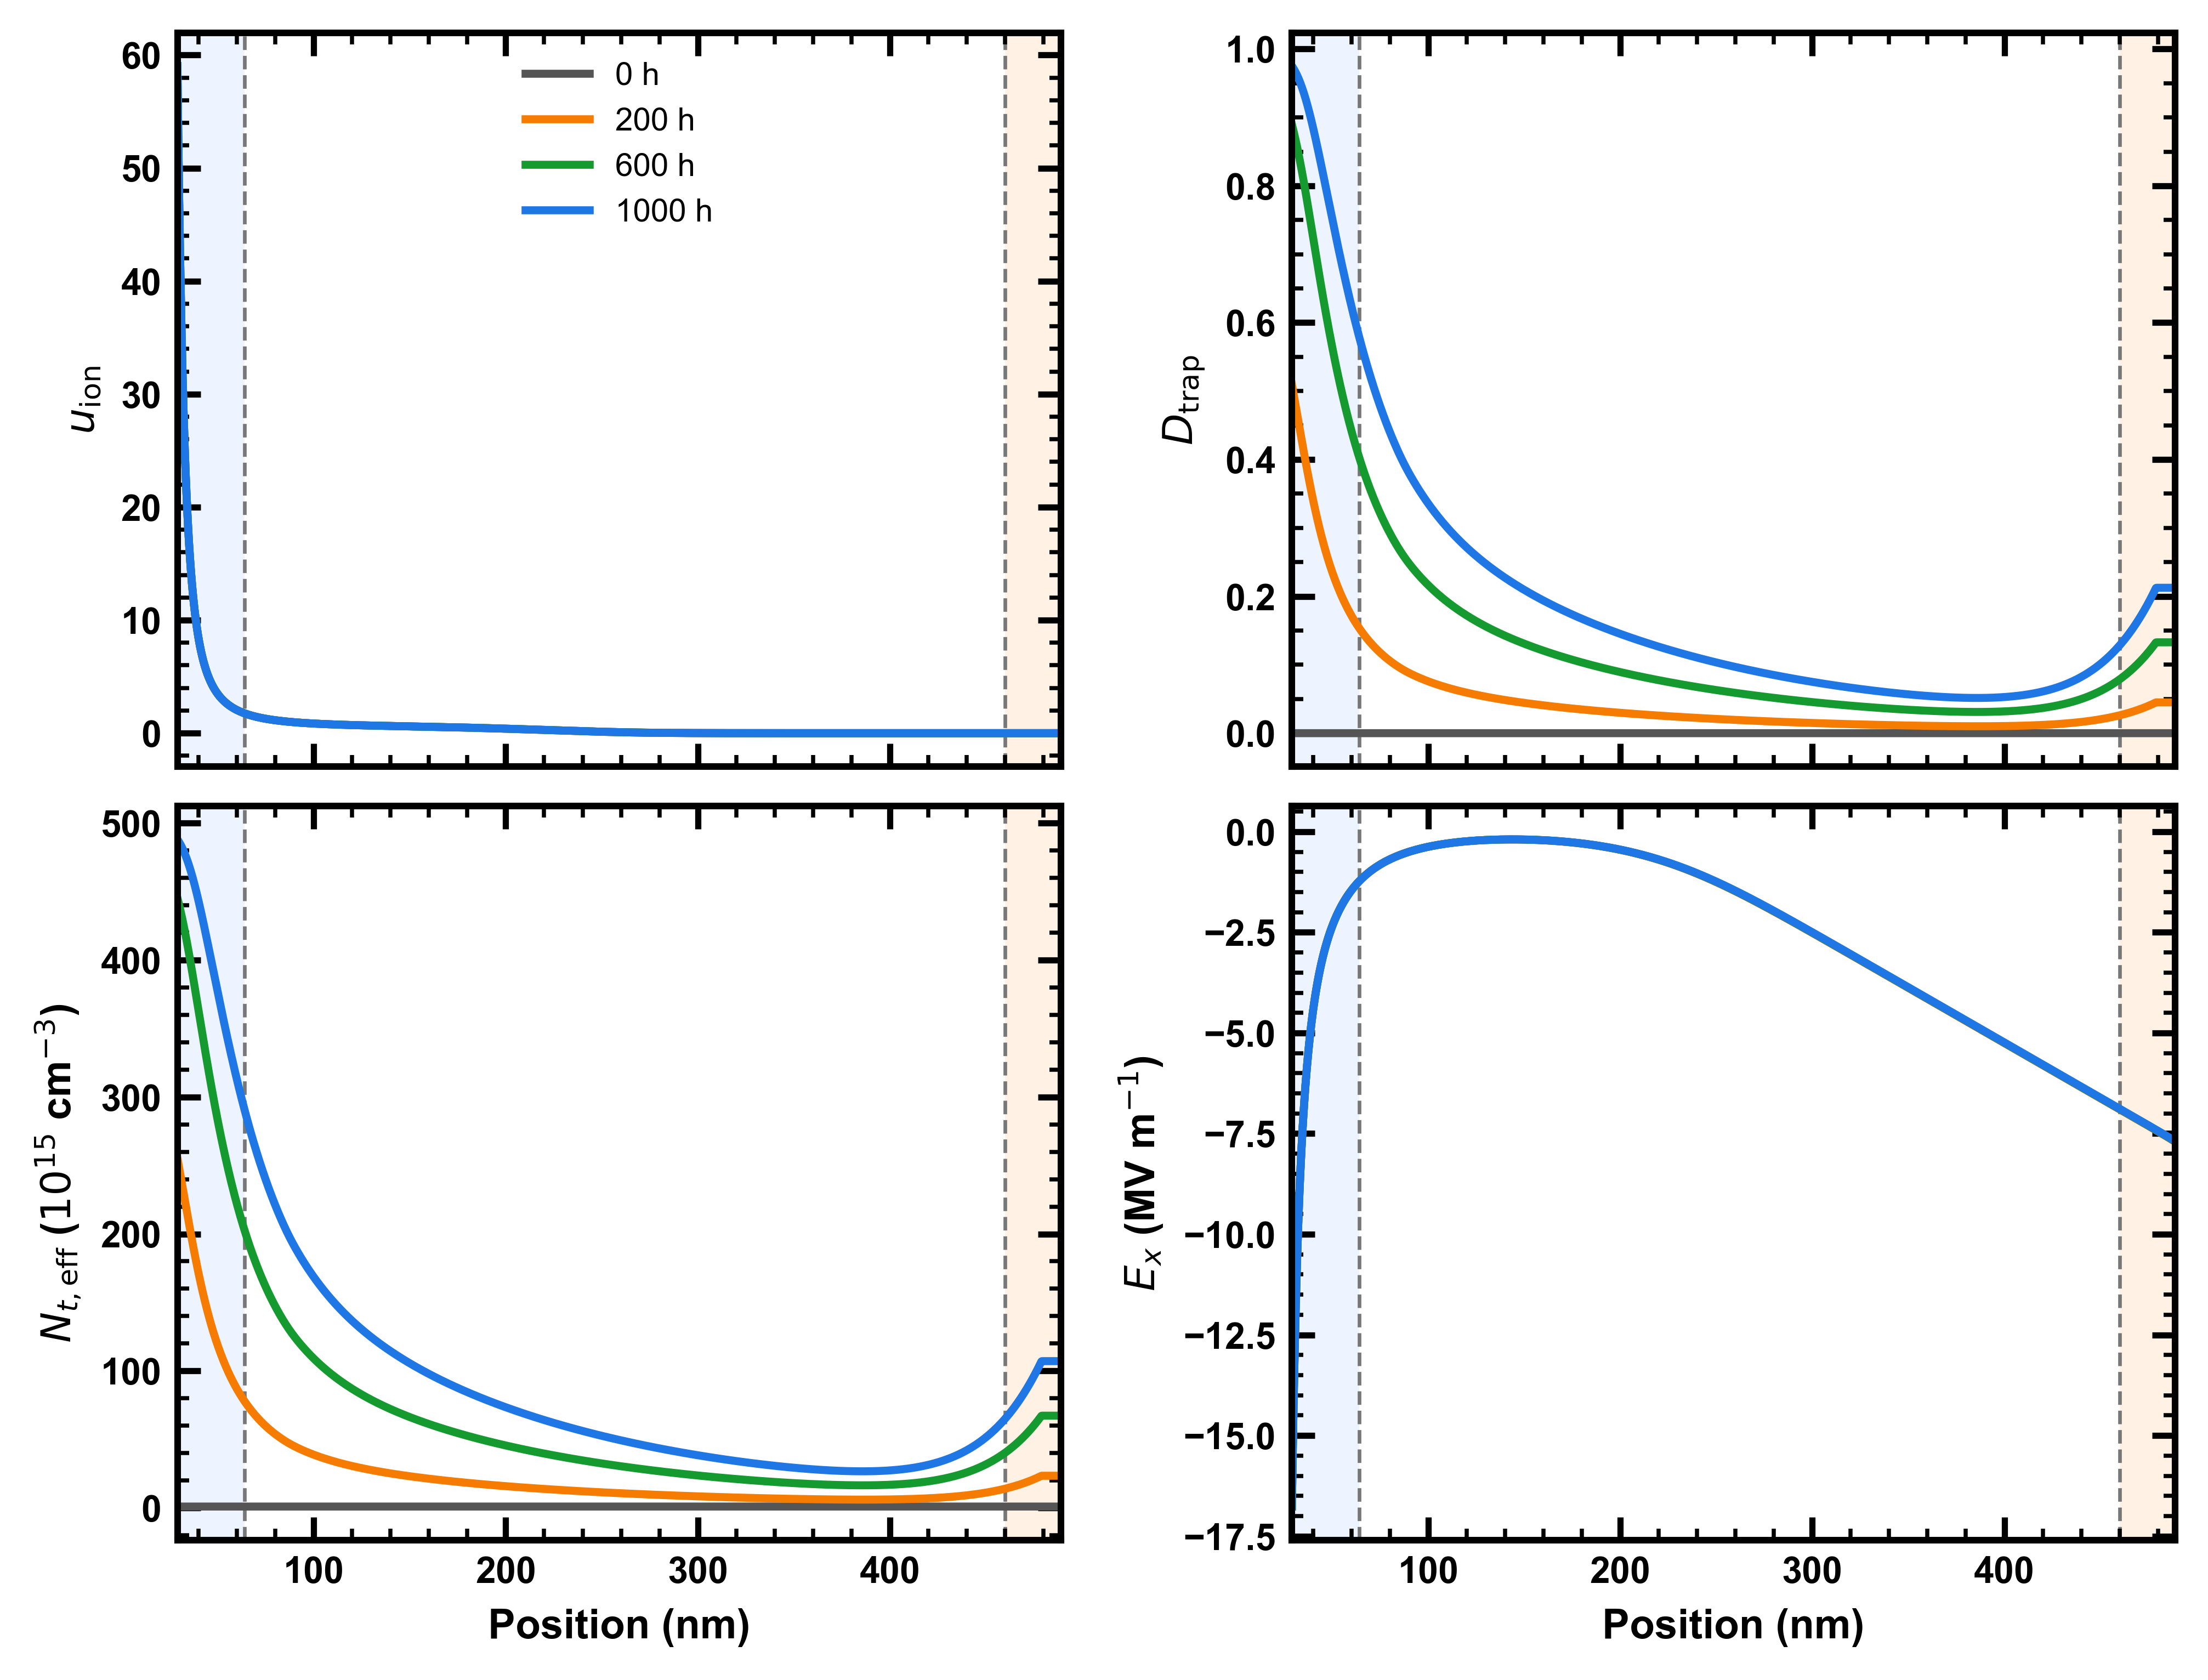
\includegraphics[width=0.92\textwidth]{outputs/figures/comsol_architecture_stress_grid/baseline_pin_spatial_profiles_high_stress_time_evolution.png}
\caption{Time evolution of the high-stress spatial profile at 1 sun and
400 K. The interface-localized increase in $D_{\mathrm{trap}}$ and
$N_{t,\mathrm{eff}}$ shows how the latent damage state maps onto an electronic
recombination parameter while the mobile-ion profile remains strongly
interfacial.}
\label{fig:spatial_profiles_high_stress}
\end{figure}

\begin{table}[H]
\centering
\caption{Selected spatial-profile summaries at 1000 h equivalent aging.}
\label{tab:spatial_profile_summary}
\begin{tabular}{@{}lrrrr@{}}
\toprule
Case & Mean $u_{\mathrm{ion}}$ & Max $u_{\mathrm{ion}}$ & Max $D_{\mathrm{trap}}$ & Mean $N_{t,\mathrm{eff}}$ (cm$^{-3}$) \\
\midrule
0 sun, 300 K & 0.27 & 1.52 & 5.16e-05 & 1.009e+15 \\
0.60 sun, 360 K & 0.287 & 1.65 & 0.0617 & 7.429e+15 \\
1.00 sun, 400 K & 0.298 & 1.72 & 0.574 & 7.488e+16 \\
\bottomrule
\end{tabular}
\end{table}


In Table~\ref{tab:spatial_profile_summary}, the perovskite-domain mean of
$u_{\mathrm{ion}}$ is a sampled-grid normalization diagnostic rather than a
strict conservation integral. Because $u_{\mathrm{ion}}=c_{\mathrm{ion}}/
c_{\mathrm{ion},0}$ is a normalized concentration, the physically relevant
conservation check is the integrated inventory ratio,
\begin{equation}
\frac{\int_{\mathrm{PVK}} c_{\mathrm{ion}}(x,t)\,dx}
{\int_{\mathrm{PVK}} c_{\mathrm{ion}}(x,0)\,dx},
\end{equation}
evaluated with the same COMSOL integration operator and domain selection used
by the model.

The first dedicated COMSOL DIT baseline-control export is shown in
Fig.~\ref{fig:dit_baseline_control}. This dark, no-scan transient has
\texttt{light\_on = 0} and \texttt{use\_scan = 0}. It captures the
electronic/capacitive switching response that must be subtracted from a
mobile-ion-active pulse before integrating ionic charge. The tail current is
near zero after the switching transient, so the export is suitable as a
background-control data product. It does not by itself define a final mobile-ion
concentration because the matched mobile-ion-active pulse must be processed
with the same time base and voltage protocol.

\begin{figure}[H]
\centering
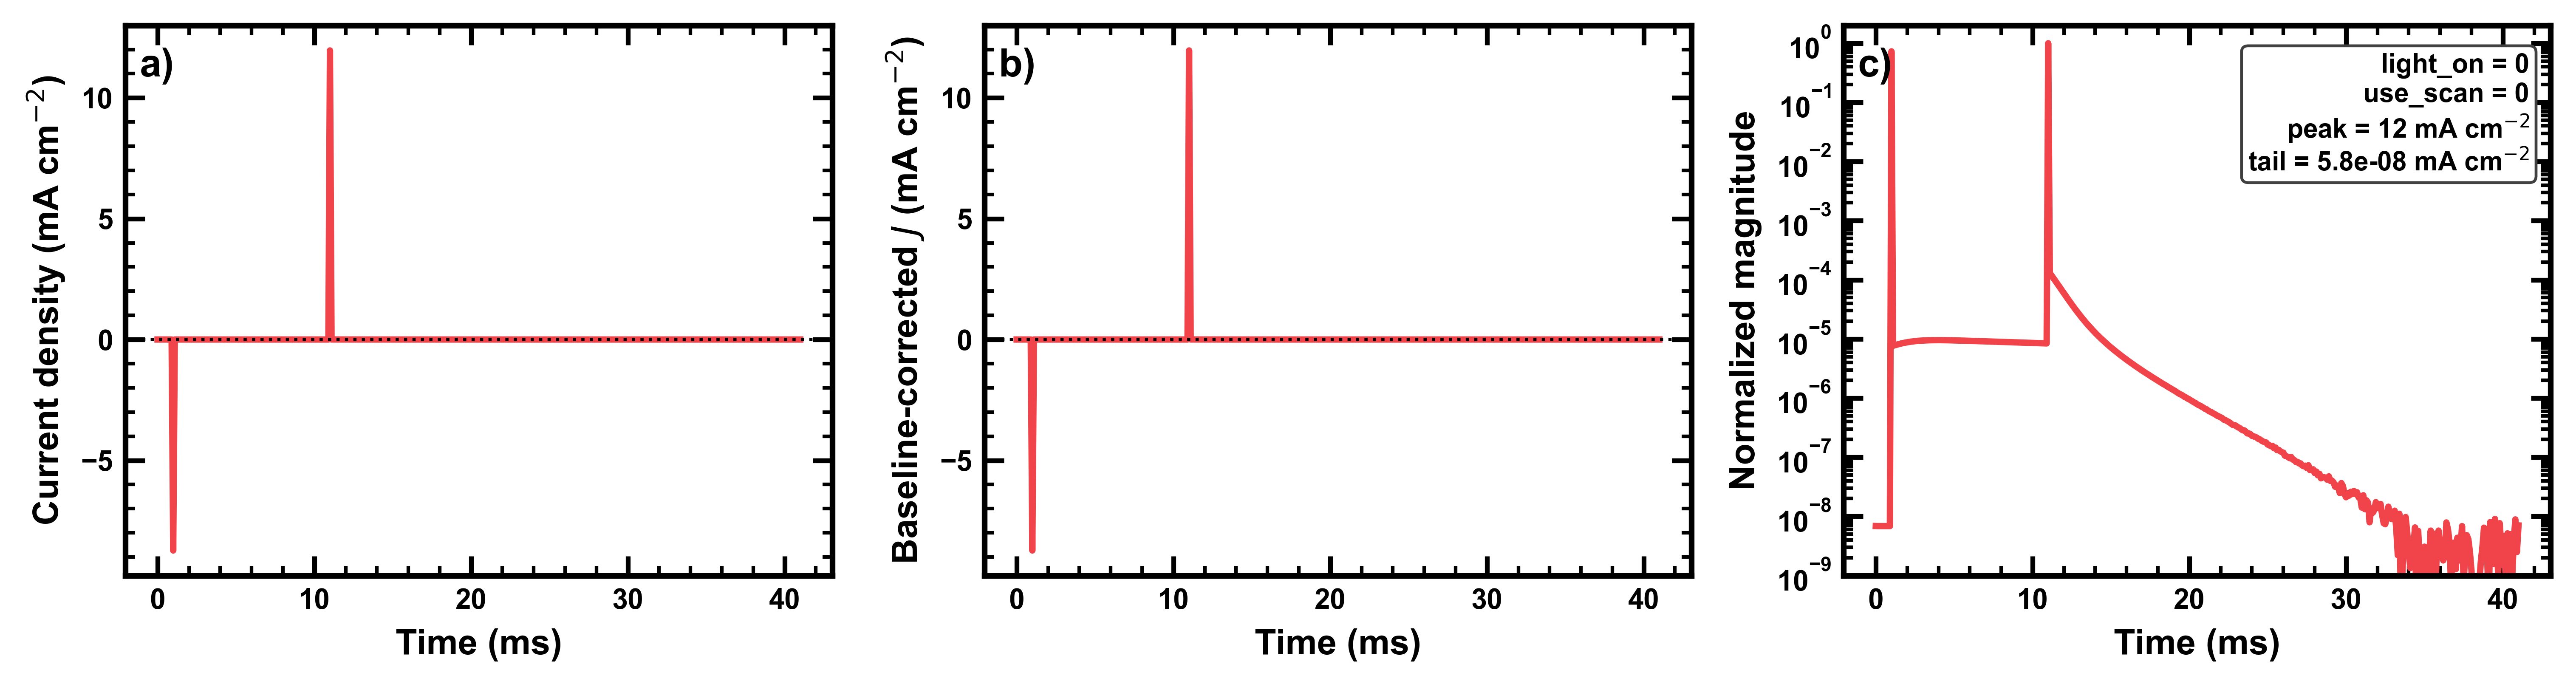
\includegraphics[width=\textwidth]{outputs/figures/dit/dit_baseline_control.png}
\caption{COMSOL DIT baseline-control transient from the dark, no-scan export.
The large switching spikes define the electronic/capacitive background, while
the post-switching tail approaches the numerical current-density floor. This
control is the required background trace for later baseline-corrected ionic
charge integration.}
\label{fig:dit_baseline_control}
\end{figure}

The DIT governing equations and extraction methods are implemented or
documented, but the quantitative ion-density result is not claimed as a final
result until the matched mobile-ion-active current is exported and baseline
subtracted against this control.

\section{Discussion}

The simulation results support the central modeling approach. The COMSOL model
connects electronic drift-diffusion, mobile-ion redistribution, and
degradation-state mappings in a single auditable framework. The strongest
qualitative result is mechanism separation: trap density, shunting, contact
resistance, photogeneration, and ionic charge produce different J--V
signatures. The main limitation is calibration. Stronger claims require matched
baseline J--V data, controlled aging data, ion-sensitive measurements, and
uncertainty estimates for the degradation amplitudes.

\chapter{Limitations, Reproducibility, and Future Work}

The thesis ends by separating current conclusions from remaining work. The
model is useful for mechanism separation and surrogate-ready data generation,
but device-specific lifetime prediction still requires stronger calibration,
ion-sensitive validation, and broader experimental constraints.

\section{Limitations}

The COMSOL model is a physics-based accelerated degradation study, not a final
lifetime prediction for a specific commercial device. The
starting electronic behavior must still be calibrated against the measured
fresh-device J--V range, and the degradation rates are accelerated for
computational practicality. The reported aging time should therefore be
interpreted as equivalent accelerated aging time, not as a direct field-time
prediction.

The second limitation is that different causes can look similar in a J--V
curve. Defect growth, leakage, contact resistance, surface recombination, and
reduced light-generated current can all lower PCE. Several combinations can
produce similar measured J--V degradation. The model needs hysteresis, impedance,
transient-current, optical, and aging data to separate these mechanisms with
confidence.

The third limitation is ion validation. The normalized ion variable
$u_{\mathrm{ion}}$ represents ion movement inside the model, but ion mobility,
concentration, boundary behavior, and the link between ion motion and defect
growth need
experimental support before they can be treated as device-specific
material parameters. DIT and capacitance-based measurements provide stronger
constraints than ordinary J--V curves, but the integrated current must be
baseline-corrected so that electronic plateaus and capacitive spikes are not
mistaken for mobile ionic charge.

The fourth limitation is implementation consistency with the laboratory stack.
The physical architecture is
glass/ITO/NiO$_x$/MeO-2PACz/perovskite/C$_{60}$/BCP/Ag/UV-resin/glass,
illuminated from the ITO side. All stack labels, domain selections,
illumination direction, coordinate conventions, and contact work functions must
remain consistent with that architecture before the model is called
device-specific.

The fifth limitation is diagnostic-voltage completeness. The light-temperature
stress-matrix J--V study is physically scaled and usable for PCE and $J_{sc}$
across all 360 curves, but its 1.25 V diagnostic voltage limit does not resolve
zero-current crossings for all mild or early-aging cases.
Quantitative $V_{oc}$ and FF claims therefore remain limited to the subset of
curves that cross zero current. A wider diagnostic voltage sweep is needed
before those quantities can be reported for every case.

\section{Reproducibility}

The analysis is organized so that the reported figures and tables can be
regenerated from the COMSOL-derived tables. The reproducibility package
separates simulation outputs, processed tables, plotting routines, thesis
source, and generated figures. Appendix~C gives the practical execution
details for rebuilding the results without interrupting the scientific
narrative in the main chapters.

\section{Data Availability}

The thesis source, processed analysis artifacts, generated figures and tables,
and public PDF are maintained in the supporting public repository at
\url{https://github.com/flabio121/thesis-public}. Large simulation
intermediates are excluded from the public copy when they are too large for
practical version control. Appendix~C and the reproducibility files document
how the public artifacts map to the underlying simulation studies.

\section{Future Work}

The next step is improved calibration. The pristine COMSOL
baseline should be fit to the same device architecture and measurement
conditions as the experimental J--V data. The fit should match $V_{oc}$,
$J_{sc}$, FF, and PCE before degradation parameters are interpreted.

The second step is implementation and validation of light-soaking and
self-healing terms. The proposed conditioning state can represent improved
contact extraction under illumination, while optional healing terms can
represent partial recovery during rest. These terms require controlled
light-soaking, dark-rest, and repeated-scan experiments before they should be
used in predictive simulations.

The third step is ion-sensitive validation. Electrical impedance spectroscopy
(EIS), transient photocurrent (TPC), capacitance, ion-current, and
scan-rate-dependent hysteresis measurements can help determine
$c_{\mathrm{ion},0}$, $\mu_{\mathrm{ion}}$, $D_{\mathrm{ion}}$, boundary
conditions, and the link between ion motion and defect growth. These
measurements are needed because ordinary J--V curves alone do not uniquely
determine the ion state.
Future DIT simulations should pair each ion-transport case with a control case
where the ions are held fixed, so that $I_{\mathrm{corr}}(t)$ and the extracted
$N_0$ are defined by the ion-related transient signal rather than by the total
measured current.

The fourth step is device-stack-specific calibration. The model should be
calibrated separately for device stacks, contacts, and barrier layers because
the same degradation pathway can produce different electrical signatures in
different architectures.

The fifth step is completion of the spatial and transient result set. The
selected spatial results now support band diagrams with carrier energy levels,
the correct HTL-to-ETL plotting direction, and selected ion and trap
line-profile panels from the profile grid. Final validation should still
include explicit short-circuit, maximum-power, and open-circuit band diagrams,
a strict COMSOL ion-conservation check, and fixed-ion-control DIT charge
extraction. The quantitative DIT result remains a future validation step until
a fixed-ion or no-ion control current is available for baseline subtraction.

The final step is a COMSOL-calibrated surrogate workbench. The current
6 $\times$ 6 light-temperature grid supports a first forward surrogate
baseline. That baseline demonstrates grouped COMSOL-to-COMSOL interpolation
for PCE, normalized PCE, PCE retention, $J_{sc}$, and J--V current density, but
it is trained only on the present COMSOL grid and is not an experimental
predictor. A later tool would need uncertainty estimates, active-learning run
selection, inverse diagnosis from measured J--V history, and matched
experimental calibration. The surrogate would speed up parameter exploration
and help infer hidden device states from measured J--V history, but it would
not replace the COMSOL drift--diffusion model as the physics reference.

\section{Concluding Perspective}

This thesis develops a COMSOL-based degradation model for perovskite solar
cells. The model links electronic transport, ion movement, defect growth,
contact resistance, leakage, voltage protocol, optical generation, DIT pulse
analysis, parameter sweeps, and accelerated J--V aging studies in one workflow.
It shows that several hidden mechanisms can produce distinct but overlapping
J--V signatures. Experimental calibration remains the main unfinished step.
Future work should focus on improved calibration, self-healing and
light-soaking terms, ion-sensitive validation, device-stack-specific
parameters, and broader COMSOL-calibrated surrogate use after the data set is
physically grounded.


% -------------------------
% REFERENCES
% -------------------------
\bibliographystyle{ieeetr}
\bibliography{refs}

% -------------------------
% APPENDICES
% -------------------------
\appendix
\chapter{COMSOL Parameter and Scenario Organization}

\section{Parameter Files}

The COMSOL-facing parameter files are stored under
\texttt{data/model\_parameters/}. The accelerated degradation study uses the
CSV parameter set for:
\begin{itemize}
\item master degradation state, \texttt{General Degradation D\_Master.csv};
\item scenario controls, \texttt{Case Study.csv};
\item series resistance, \texttt{Series Resistance Rs.csv};
\item shunt resistance, \texttt{Shunt Resistance Rsh.csv};
\item trap density, \texttt{Trap Density Nt (Bulk Recomb).csv};
\item mobile/interfacial charge, \texttt{Mobile Ions.csv}; and
\item surface recombination, \texttt{Surface Recomb S.csv}.
\end{itemize}

The accelerated amplitudes are intentionally strong enough to make the full
coupled case cross $T_{80}$ before 3000 h. This makes the library suitable for
mechanism sensitivity and calibration planning.

\section{Architecture Parameters}

The laboratory stack is
\begin{equation}
\mathrm{glass}/\mathrm{ITO}/\mathrm{NiO}_x/
\mathrm{MeO\mbox{-}2PACz}/\mathrm{MHP}/
\mathrm{C}_{60}/\mathrm{BCP}/\mathrm{Ag}/
\mathrm{UV\ resin}/\mathrm{glass}.
\end{equation}
The reduced electronic geometry uses the following model parameters:
\begin{itemize}
\item \texttt{thickness\_HTL = 35[nm]};
\item \texttt{thickness\_PVK = 450[nm]}; and
\item \texttt{thickness\_ETL = 29[nm]}.
\end{itemize}
The HTL combines approximately 30 nm NiO$_x$
and 5 nm MeO-2PACz; the ETL combines approximately 25 nm C$_{60}$ and 4 nm
BCP. The 100 nm Ag layer, ITO, resin, and glass are represented as contacts,
illumination context, or omitted encapsulation rather than semiconductor
transport domains.

\section{Scenario Semantics}

\begin{table}[H]
\centering
\begin{tabular}{lll}
\toprule
Mode & Case ID & Meaning \\
\midrule
0 & 0 & full coupled degradation \\
1 & 0 & all-off control \\
1 & 1--5 & one-only mechanism case \\
0 & 1--5 & leave-one-out mechanism case \\
\bottomrule
\end{tabular}
\caption{Scenario semantics used by the COMSOL sweep and processing pipeline.}
\label{tab:scenario_semantics}
\end{table}

For \texttt{case\_id=1..5}, the selected mechanisms are $R_s$, $R_{sh}$,
$N_t$, $Q_f$, and $S$.

\section{Generated Data Products}

The primary processed COMSOL products are:
\begin{itemize}
\item \texttt{data/processed/comsol/comsol\_scenario\_lookup.csv};
\item \texttt{data/processed/comsol/comsol\_scenario\_timeseries.csv};
\item \texttt{data/processed/comsol/comsol\_lifetime\_summary.csv};
\item \texttt{outputs/figures/comsol\_baseline\_pce.png};
\item \texttt{outputs/figures/comsol\_full\_jv\_evolution.png};
\item \texttt{outputs/figures/comsol\_mechanism\_sensitivity.png};
\item \texttt{outputs/figures/comsol\_metric\_signatures.png}; and
\item \texttt{outputs/figures/comsol\_state\_trajectories.png}.
\end{itemize}

These files are regenerated by
\texttt{scripts/run\_comsol\_paper\_pipeline.py}.

\section{Electronic Parameter-Sweep Products}

The separate electronic parameter sweep uses the COMSOL Global Evaluation data
under \path{data/raw/comsol/}:
\begin{verbatim}
arch_baseline_pin/parameter_sweeps/comsol_pscdeg_sweep_001.csv
\end{verbatim}
and is processed by
\begin{verbatim}
python .\scripts\plot_comsol_parameter_sweep.py
\end{verbatim}
The script writes:
\begin{itemize}
\item \path{outputs/tables/comsol_parameter_sweep_metrics.csv};
\item \path{outputs/tables/comsol_parameter_sweep_single_axis_metrics.csv};
\item combined J--V and metric figures under
\path{outputs/figures/comsol_parameter_sweep/};
\item the combined J--V examples figure and combined metric-grid figure; and
\item individual PDF, PNG, and SVG panels for the $N_{t,0}$, $R_{s,0}$, and
$R_{sh,0}$ sweeps in the same directory.
\end{itemize}
This sweep is a baseline electronic-parameter sensitivity study, not an aging
or lifetime simulation.

\section{Architecture-Stress Data Products}

The baseline architecture aging data are stored under the architecture folder
\path{arch_baseline_pin/Aging/}. The canonical light-temperature stress-matrix
J--V data file is:
\begin{verbatim}
Stress_matrix_jv_003.csv
\end{verbatim}
and is processed by:
\begin{verbatim}
python .\scripts\process_comsol_architecture_stress_jv.py
\end{verbatim}
The resulting tables and figures use the prefix
\path{baseline_pin_stress_matrix_jv_003_}. Superseded development data are
kept only in the repository audit trail and are not used for current
quantitative claims.

The internal-state profile grid is stored in:
\begin{verbatim}
arch_baseline_pin/Aging/profile_grid_light_temperature/
\end{verbatim}
It covers 300--400 K and 0.01--1.00 sun, with canonical filenames and an
original-file manifest. The grid is processed with:
\begin{verbatim}
python .\scripts\process_comsol_profile_grid.py
\end{verbatim}
and writes the long-format state summary under
the architecture-stress processed-data folder.

\chapter{Observable and Mechanism Mapping}

This appendix records how measured or simulated observables constrain the
COMSOL model states. The mapping is not one-to-one; it identifies which
measurements best constrain each physical mechanism.

\begin{table}[H]
\centering
\begin{tabular}{p{0.22\textwidth}p{0.34\textwidth}p{0.32\textwidth}}
\toprule
Observable & Primary sensitivity & COMSOL use \\
\midrule
Normalized PCE & aggregate performance loss & aging trajectory and $T_{80}$ marker \\
$V_{oc}$ & recombination and electrostatic shifts & trap density, surface recombination, and charge calibration \\
$J_{sc}$ & collection and absorber-quality changes & photogeneration, collection, and strong recombination check \\
FF & leakage, shunting, contact, and curve-shape losses & $R_s$, $R_{sh}$, and interface-loss calibration \\
$V_{mpp}$, $J_{mpp}$ & operating-point shift & maximum-power-point and deployment relevance \\
Hysteresis index & mobile ions and field redistribution & $c_{\mathrm{ion},0}$, $\mu_{\mathrm{ion}}$, and boundary-condition calibration \\
PL peak shift & composition and bandgap change & absorber-state and photogeneration-loss constraint \\
PL spread & spatial heterogeneity & check against the one-dimensional uniformity assumption \\
XRD phase fraction & composition or secondary phases & absorber degradation and phase-segregation constraint \\
Impedance or transient current & ions, capacitance, and interface dynamics & ion mobility, ion density, and interface-state calibration \\
\bottomrule
\end{tabular}
\caption{Observation mapping for COMSOL degradation calibration.}
\label{tab:feature_state_mapping}
\end{table}

The table defines calibration targets rather than fitted proof. Terminal J--V
data are necessary but not sufficient because several mechanisms can produce
similar PCE loss. Hysteresis, impedance, transient current, PL, and XRD
measurements provide additional constraints that help separate ionic,
recombination, contact, leakage, and absorber-quality changes.

\chapter{Repository Workflow}

\section{Primary COMSOL Processing Workflow}

The primary processing workflow is:
\begin{enumerate}
\item export COMSOL J--V and state tables to
\texttt{data/raw/comsol/time\_series/};
\item run:
\begin{verbatim}
python .\scripts\run_comsol_paper_pipeline.py
\end{verbatim}
\item inspect processed data under \texttt{data/processed/comsol/};
\item inspect generated figures under \texttt{outputs/figures/}; and
\item rebuild the thesis with
\texttt{latexmk -pdf -interaction=nonstopmode main.tex}.
\end{enumerate}

\section{Traceability Files}

The repository includes support files for reproducibility and archival use:
\begin{itemize}
\item \texttt{README.md};
\item \texttt{START\_HERE.md};
\item \texttt{REPRODUCIBILITY.md};
\item \texttt{docs/data\_dictionary.md};
\item \texttt{docs/traceability\_matrix.md};
\item \texttt{docs/journal\_submission\_checklist.md}; and
\item \texttt{CITATION.cff}.
\end{itemize}

\section{External Calibration Context}

The external Wang et al. source-data workflow can be run as supporting
calibration context:
\begin{verbatim}
python .\scripts\run_psc_degradation_study.py
\end{verbatim}
That workflow is not the central thesis result. The central result is the
COMSOL model, the processed COMSOL scenario library, the mechanism-specific
parameter mappings, and the experimental calibration plan.

\section{Electronic Parameter-Sweep Workflow}

The uploaded COMSOL Global Evaluation sweep for $N_{t,0}$, $R_{s,0}$, and
$R_{sh,0}$ is processed separately from the aging-time pipeline:
\begin{verbatim}
python .\scripts\plot_comsol_parameter_sweep.py
\end{verbatim}
This command reads the architecture-scoped parameter-sweep export under
\path{data/raw/comsol/arch_baseline_pin/parameter_sweeps/}, extracts the active
voltage-ramp segment for each parameter combination, computes J--V metrics, and
writes sweep figures under
\path{outputs/figures/comsol_parameter_sweep/}. It also writes:
\begin{itemize}
\item \path{outputs/tables/comsol_parameter_sweep_metrics.csv}; and
\item \path{outputs/tables/comsol_parameter_sweep_single_axis_metrics.csv}.
\end{itemize}

\section{Surrogate Workbench Prototype}

The supporting surrogate application is launched with:
\begin{verbatim}
streamlit run .\apps\psc_surrogate_app\streamlit_app.py
\end{verbatim}
The current application uses placeholder prediction logic and current COMSOL
seed tables. Its purpose is to define the future data contract, run
provenance, export bundle format, inverse-diagnosis interface, and
active-learning workflow before the full COMSOL design of experiments is
available.

\section{Architecture-Stress Grid Workflow}

The architecture-scoped aging exports are processed with:
\begin{verbatim}
python .\scripts\process_comsol_architecture_stress_jv.py
python .\scripts\process_comsol_profile_grid.py
\end{verbatim}
The first command extracts diagnostic J--V curves and PV metrics from the
baseline p-i-n temperature-aging exports. The second command summarizes the
6 $\times$ 6 light-temperature profile grid into condition-time-variable rows
with spatial means, extrema, and interface-region summaries. The profile-grid
summary is the current bridge between COMSOL internal states and future
surrogate or inverse-diagnosis data sets.


\end{document}
